


\documentclass[12pt,twoside]{report}

\usepackage{amsfonts,amsmath,amssymb,stmaryrd,indentfirst}
\usepackage{epsfig,graphicx,times,psfrag}
\usepackage{natbib,enumerate}
%\usepackage{fancyhdr} %%%%
\usepackage{color}
\usepackage{fullpage}
\usepackage{helvet}
%\pagestyle{fancy}%%%%
\usepackage[pdftex,bookmarks,colorlinks=true,urlcolor=rltblue,citecolor=blue]{hyperref}
\def\newblock{\hskip .11em plus .33em minus .07em}

\setlength\textwidth      {16.5cm}
\setlength\textheight     {22.0cm}
\setlength\oddsidemargin  {-0.3cm}
\setlength\evensidemargin {-0.3cm}

\setlength\headheight{0in} 
\setlength\topmargin{0.cm}
\setlength\headsep{1.cm}
\setlength\footskip{1.cm}
\setlength\parskip{0pt}

%%%%%%%%%%%%%%%%%%%%%%%%%%%%%%%%%%%%%%%%%%%
%%%%%%                              %%%%%%%
%%%%%%      NOTATION SECTION        %%%%%%%
%%%%%%                              %%%%%%%
%%%%%%%%%%%%%%%%%%%%%%%%%%%%%%%%%%%%%%%%%%%

% Text abbreviations.
\newcommand{\ie}{{\em{i.e., }}}
\newcommand{\eg}{{\em{e.g., }}}
\newcommand{\cf}{{\em{cf., }}}
\newcommand{\wrt}{with respect to}
\newcommand{\lhs}{left hand side}
\newcommand{\rhs}{right hand side}
% Commands definining mathematical notation.

% This is for quantities which are physically vectors.
\renewcommand{\vec}[1]{{\mbox{\boldmath$#1$}}}
% Physical rank 2 tensors
\newcommand{\tensor}[1]{\overline{\overline{#1}}}
% This is for vectors formed of the value of a quantity at each node.
\newcommand{\dvec}[1]{\underline{#1}}
% This is for matrices in the discrete system.
\newcommand{\mat}[1]{\mathrm{#1}}


\DeclareMathOperator{\sgn}{sgn}
\newtheorem{thm}{Theorem}[section]
\newtheorem{lemma}[thm]{Lemma}

%\newcommand\qed{\hfill\mbox{$\Box$}}
\newcommand{\re}{{\mathrm{I}\hspace{-0.2em}\mathrm{R}}}
\newcommand{\inner}[2]{\langle#1,#2\rangle}
\renewcommand\leq{\leqslant}
\renewcommand\geq{\geqslant}
\renewcommand\le{\leqslant}
\renewcommand\ge{\geqslant}
\renewcommand\epsilon{\varepsilon}
\newcommand\eps{\varepsilon}
\renewcommand\phi{\varphi}
\newcommand{\bmF}{\vec{F}}
\newcommand{\bmphi}{\vec{\phi}}
\newcommand{\bmn}{\vec{n}}
\newcommand{\bmns}{{\textrm{\scriptsize{\boldmath $n$}}}}
\newcommand{\bmi}{\vec{i}}
\newcommand{\bmj}{\vec{j}}
\newcommand{\bmk}{\vec{k}}
\newcommand{\bmx}{\vec{x}}
\newcommand{\bmu}{\vec{u}}
\newcommand{\bmv}{\vec{v}}
\newcommand{\bmr}{\vec{r}}
\newcommand{\bma}{\vec{a}}
\newcommand{\bmg}{\vec{g}}
\newcommand{\bmU}{\vec{U}}
\newcommand{\bmI}{\vec{I}}
\newcommand{\bmq}{\vec{q}}
\newcommand{\bmT}{\vec{T}}
\newcommand{\bmM}{\vec{M}}
\newcommand{\bmtau}{\vec{\tau}}
\newcommand{\bmOmega}{\vec{\Omega}}
\newcommand{\pp}{\partial}
\newcommand{\kaptens}{\tensor{\kappa}}
\newcommand{\tautens}{\tensor{\tau}}
\newcommand{\sigtens}{\tensor{\sigma}}
\newcommand{\etens}{\tensor{\dot\epsilon}}
\newcommand{\ktens}{\tensor{k}}
\newcommand{\half}{{\textstyle \frac{1}{2}}}
\newcommand{\tote}{E}
\newcommand{\inte}{e}
\newcommand{\strt}{\dot\epsilon}
\newcommand{\modu}{|\bmu|}
% Derivatives
\renewcommand{\d}{\mathrm{d}}
\newcommand{\D}{\mathrm{D}}
\newcommand{\ddx}[2][x]{\frac{\d#2}{\d#1}}
\newcommand{\ddxx}[2][x]{\frac{\d^2#2}{\d#1^2}}
\newcommand{\ddt}[2][t]{\frac{\d#2}{\d#1}}
\newcommand{\ddtt}[2][t]{\frac{\d^2#2}{\d#1^2}}
\newcommand{\ppx}[2][x]{\frac{\partial#2}{\partial#1}}
\newcommand{\ppxx}[2][x]{\frac{\partial^2#2}{\partial#1^2}}
\newcommand{\ppt}[2][t]{\frac{\partial#2}{\partial#1}}
\newcommand{\pptt}[2][t]{\frac{\partial^2#2}{\partial#1^2}}
\newcommand{\DDx}[2][x]{\frac{\D#2}{\D#1}}
\newcommand{\DDxx}[2][x]{\frac{\D^2#2}{\D#1^2}}
\newcommand{\DDt}[2][t]{\frac{\D#2}{\D#1}}
\newcommand{\DDtt}[2][t]{\frac{\D^2#2}{\D#1^2}}
% Norms
\newcommand{\Ltwo}{\ensuremath{L_2} }
% Basis functions
\newcommand{\Qone}{\ensuremath{Q_1} }
\newcommand{\Qtwo}{\ensuremath{Q_2} }
\newcommand{\Qthree}{\ensuremath{Q_3} }
\newcommand{\QN}{\ensuremath{Q_N} }
\newcommand{\Pzero}{\ensuremath{P_0} }
\newcommand{\Pone}{\ensuremath{P_1} }
\newcommand{\Ptwo}{\ensuremath{P_2} }
\newcommand{\Pthree}{\ensuremath{P_3} }
\newcommand{\PN}{\ensuremath{P_N} }
\newcommand{\Poo}{\ensuremath{P_1P_1} }
\newcommand{\PoDGPt}{\ensuremath{P_{-1}P_2} }

\newcommand{\metric}{\tensor{M}}
\newcommand{\configureflag}[1]{\texttt{#1}}

% Units
\newcommand{\m}[1][]{\unit[#1]{m}}
\newcommand{\km}[1][]{\unit[#1]{km}}
\newcommand{\s}[1][]{\unit[#1]{s}}
\newcommand{\invs}[1][]{\unit[#1]{s}\ensuremath{^{-1}}}
\newcommand{\ms}[1][]{\unit[#1]{m\ensuremath{\,}s\ensuremath{^{-1}}}}
\newcommand{\mss}[1][]{\unit[#1]{m\ensuremath{\,}s\ensuremath{^{-2}}}}
\newcommand{\K}[1][]{\unit[#1]{K}}
\newcommand{\PSU}[1][]{\unit[#1]{PSU}}
\newcommand{\Pa}[1][]{\unit[#1]{Pa}}
\newcommand{\kg}[1][]{\unit[#1]{kg}}
\newcommand{\rads}[1][]{\unit[#1]{rad\ensuremath{\,}s\ensuremath{^{-1}}}}
\newcommand{\kgmm}[1][]{\unit[#1]{kg\ensuremath{\,}m\ensuremath{^{-2}}}}
\newcommand{\kgmmm}[1][]{\unit[#1]{kg\ensuremath{\,}m\ensuremath{^{-3}}}}
\newcommand{\Nmm}[1][]{\unit[#1]{N\ensuremath{\,}m\ensuremath{^{-2}}}}

% Dimensionless numbers
\newcommand{\dimensionless}[1]{\mathrm{#1}}
\renewcommand{\Re}{\dimensionless{Re}}
\newcommand{\Ro}{\dimensionless{Ro}}
\newcommand{\Fr}{\dimensionless{Fr}}
\newcommand{\Bu}{\dimensionless{Bu}}
\newcommand{\Ri}{\dimensionless{Ri}}
\renewcommand{\Pr}{\dimensionless{Pr}}
\newcommand{\Pe}{\dimensionless{Pe}}
\newcommand{\Ek}{\dimensionless{Ek}}
\newcommand{\Gr}{\dimensionless{Gr}}
\newcommand{\Ra}{\dimensionless{Ra}}
\newcommand{\Sh}{\dimensionless{Sh}}
\newcommand{\Sc}{\dimensionless{Sc}}

% Added macros
\newcommand{\mathbi}[1]{\boldsymbol{ #1 }}
\newcommand{\fracp}[2]{\frac{\partial #1}{\partial #2}}
\newcommand{\fracd}[2]{\frac{\mathrm{d} #1}{\mathrm{d} #2}}
\renewcommand{\d}[1]{\mathrm{d} #1}
\newcommand{\Ma}{\mathrm{M\! a}}

% Journals
\newcommand{\IJHMT}{{\it International Journal of Heat and Mass Transfer}}
\newcommand{\NED}{{\it Nuclear Engineering and Design}}
\newcommand{\ICHMT}{{\it International Communications in Heat and Mass Transfer}}
\newcommand{\NET}{{\it Nuclear Engineering and Technology}}
\newcommand{\HT}{{\it Heat Transfer}}   
\newcommand{\IJHT}{{\it International Journal for Heat Transfer}}

\newcommand{\frc}{\displaystyle\frac}
\newcommand{\uline}[1]{\rule[0pt]{#1}{0.4pt}}% Fill this blank

%%%%%%%%%%%%%%%%%%%%%%%%%%%%%%%%%%%%%%%%%%%
%%%%%%                              %%%%%%%
%%%%%% END OF THE NOTATION SECTION  %%%%%%%
%%%%%%                              %%%%%%%
%%%%%%%%%%%%%%%%%%%%%%%%%%%%%%%%%%%%%%%%%%%


% Cause numbering of subsubsections. 
%\setcounter{secnumdepth}{8}
%\setcounter{tocdepth}{8}

\setcounter{secnumdepth}{4}%
\setcounter{tocdepth}{4}%

\DeclareMathAlphabet{\mathpzc}{OT1}{pzc}{m}{it}

\begin{document}


\setcounter{page}{1}

\vfill

\pagebreak


\begin{center}
{\Large Solution of the Problems -- Exam (May 2012/13)}
\end{center}

\begin{description}

%%%
%%% Module 01
%%%
\item [Question 1:] Reheat Rankine cycle with two turbines:
%\renewcommand{\theenumi}{\Alph{enumi}}
\begin{enumerate}[(a)]

\item \label{Q1}In order to fill the Table we need to calculate the thermodynamic properties for each stage of the cycle 

\begin{figure}[h]
\begin{center}
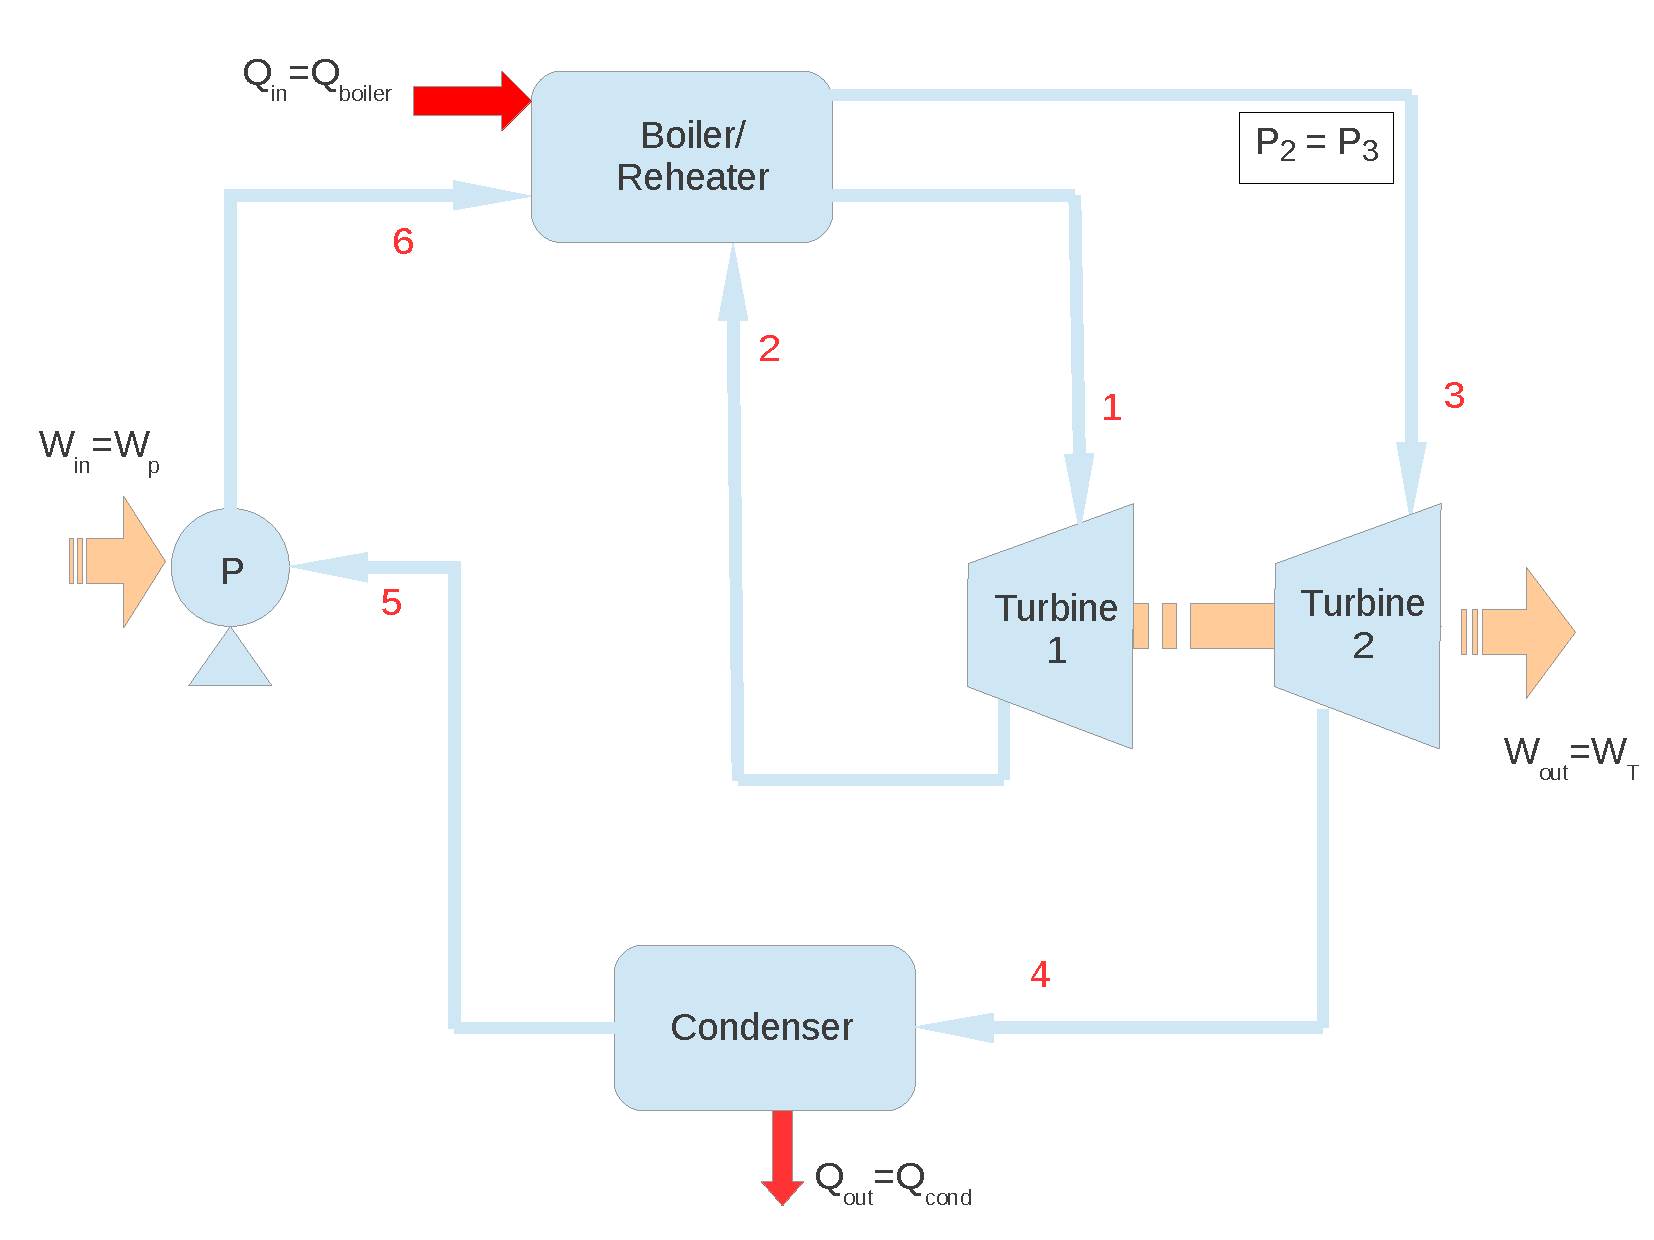
\includegraphics[width=10.cm,clip]{./Pics/Exam_Reheat_Rankine_Cycle}
\caption{ Reheat Rankine cycle with 2 turbines.}
\label{exam_mod01_rankinecycle}
\end{center}
\end{figure}

\begin{description}

%%%
\item [Stage 1:] The fluid leaving the boiler towards the first turbine is at 40 bar and 370$^{o}$C. This is well above the saturation temperature $\left(T_{\text{sat}}=250.3^{\text{o}}\text{C}\right)$ and we can thus confirm (as outlined in the given Table) that the fluid is superheated steam. At such pressure, the superheated steam tables (SHST) give,
\begin{center}
\begin{tabular}{c c c}
{\bf T $\left(^{\text{o}}\text{C}\right)$} & {\bf H (kJ/kg)}  & {\bf S (kJ/(kg.K))} \\ 
350                                      & 3092.5           & 6.582               \\
400                                      & 3213.6           & 6.769               \\ 
\end{tabular}
\end{center}
Thus, with linear interpolation at $T_{1}=370^{\text{o}}\text{C}$ for $H_{1}$ and $S_{1}$,
\begin{eqnarray}
&& H_{i} = H_{0} + \frc{T_{i}-T_{0}}{T_{1}-T_{0}}\left(H_{1}-H_{0}\right) = 3092.5 + \frc{370-350}{400-350}\left(3213.6-3092.5\right) \nonumber \\
&& \text{ or } \nonumber \\
&& H_{i} = H_{1} - \frc{T_{1}-T_{i}}{T_{1}-T_{0}}\left(H_{1}-H_{0}\right) = 3213.6 - \frc{400-370}{400-350}\left(3213.6-3092.5\right) \nonumber 
\end{eqnarray}
This leads to \textcolor{red}{$H_{1}=3140.94\frc{kJ}{kg}$} \textcolor{blue}{(1 Mark)} and \textcolor{red}{$S_{1}=6.6568\frc{kJ}{kg.K}$} \textcolor{blue}{(1 Mark)}.

%%%
\item [Stage 2:] Isentropic expansion in {\it Turbine 1} at $P_{2}=P_{3}=7\; bar \Leftrightarrow \;\; S_{2s}=S_{1}=6.6568\frc{kJ}{kg.K}$.  The fluid can be either \textcolor{red}{saturated steam} or \textcolor{red}{2 phase (steam + liquid) fluid} \textcolor{blue}{(1 Mark)}. From the saturated water-steam table (SWST),
\begin{center}
\begin{tabular}{l r c l r}
         & {\bf (kJ/kg)}  &  &          & {\bf (kJ/(kg.K))} \\
$H_{f}$   & 697.1          &  & $S_{f}$  & 1.9918 \\
%$H_{fg}$  & 2064.9        &   & $S_{fg}$ & 4.7134 \\
$H_{g}$   & 2762.0        &   & $S_{g}$  & 6.7052  \\
\end{tabular}
\end{center}
We need to alculate the quality of the ideal fluid, $X_{2s}$,
\begin{displaymath}
X_{2s} = \frc{S_{2s}-S_{f}}{S_{g}-S_{f}} = 0.9897
\end{displaymath}
Now that we know $X_{2s}$, we can determine the ideal enthalpy,
\begin{displaymath}
X_{2s}=0.9897=\frc{H_{2s}-H_{f}}{H_{g}-H_{f}} \Leftrightarrow \;\;  H_{2s} = 2740.73 \frc{kJ}{kg}
\end{displaymath}
The efficiency associated with {\it Turbine 1} is 84$\%$ thus,
\begin{displaymath}
\eta_{T1} = \frc{H_{2}-H_{1}}{H_{2s}-H_{1}} = 0.84 \Leftrightarrow \;\;  H_{2}=2804.76 \frc{kJ}{kg}
\end{displaymath}

%%%
\item [Stage 3:] The reheated steam is at 7 bar $\left(T_{\text{sat}}=165^{\text{o}}\text{C}\right)$ and 370$^{o}$C is also superheated and from SHST,
\begin{center}
\begin{tabular}{c c c}
{\bf T $\left(^{\text{o}}\text{C}\right)$} & {\bf H (kJ/kg)}  & {\bf S (kJ/(kg.K))} \\ 
350                                      & 3163.7           & 7.473      \\
400                                      & 3268.7           & 7.635      \\
\end{tabular}
\end{center}
From linear interpolation, at $T_{1}=370^{\text{o}}\text{C}$: \textcolor{red}{$H_{3}=3205.7\frc{kJ}{kg}$} \textcolor{blue}{(1 Mark)} and \textcolor{red}{$S_{3}=7.5378\frc{kJ}{kg.K}$} \textcolor{blue}{(1 Mark)}


%%%
\item [Stage 4:] The fluid that leaves the second turbine is a saturated steam at 0.10 bar with $S_{4s}=S_{3}=7.5378\frc{kJ}{kg.K}$. At this pressure the SWST gives
\begin{center}
\begin{tabular}{ l l l }
$V_{f}=0.00101 \frc{m^{3}}{kg}$  &  $H_{f}=191.8\frc{kJ}{kg}$   & $S_{f} = 0.649 \frc{kJ}{kg.K}$ \\
$V_{g}=14.67 \frc{m^{3}}{kg}$    &  $H_{g}=2584.7\frc{kJ}{kg}$  & $S_{g} = 8.150 \frc{kJ}{kg.K}$ \\
\end{tabular}
\end{center}

Calculating the quality of the fluid, $X_{4s}$,
\begin{displaymath}
X_{4s} = \frc{S_{4s}-S_{f}}{S_{g}-S_{f}} = 0.9184
\end{displaymath}
Now calculating the enthalpy of the ideal fluid,
\begin{displaymath}
X_{4s} = \frc{H_{4s}-H_{f}}{H_{g}-H_{f}} \Leftrightarrow \;\; H_{4s} = 2389.35 \frc{kJ}{kg}
\end{displaymath}
For {\it Tubine 2}, the associated efficiency is of 80$\%$,
\begin{displaymath}
\eta_{T2}=\frc{H_{4}-H_{3}}{H_{4s}-H_{3}}=0.80 \Leftrightarrow \;\; H_{4}=2552.69 \frc{kJ}{kg}
\end{displaymath}

%%%
\item [Stage 5:] The fluid after the \underline{condenser} is a \textcolor{red}{saturated water (liquid)} \textcolor{blue}{(1 Mark)} at 0.10 bar with the following characteristics:
\begin{eqnarray}
&& \textcolor{red}{H_{5}=191.8\frc{kJ}{kg}}=H_{f}\;\;\;\textcolor{blue}{(1\; Mark)} \nonumber \\
&& \textcolor{red}{S_{5}=0.649\frc{kJ}{kg.K}}=S_{f}\;\;\;\textcolor{blue}{(1\; Mark)} \nonumber \\
&& V_{5} = 0.00101 \frc{m^{3}}{kg} = V_{f} \nonumber
\end{eqnarray}

%%%
\item [Stage 6:] Finally, the fluid leaving the boiler feed \underline{pump} is a \textcolor{red}{saturated water (liquid)} \textcolor{blue}{(1 Mark)} at 40 bar. The pump has an efficiency of 61$\%$ and assuming that the water is nearly incompressible,
\begin{eqnarray}
\textcolor{red}{H_{6}} &\approx& H_{5} + V_{5} \frc{P_{6}-P_{5}}{\eta_{P}} \nonumber \\
     &\approx& 191.8 \frc{kJ}{kg} + 0.00101 \frc{m^{3}}{kg}\left(40-0.10\right)\text{bar} \times \frc{10^{5} kg/\left(m.s^{2}\right)}{1\text{ bar }} \times \frc{10^{-3} \frc{kJ}{kg}}{m^{2}/s^{2}}\times \frc{1}{0.61} \nonumber \\
     &\approx& \textcolor{red}{198.41\;\frc{kJ}{kg}}\;\;\textcolor{blue}{(1\; Mark)} \nonumber
\end{eqnarray}
%
\end{description}

Thus the Table becomes:
%\begin{table}[]
\begin{center}
\begin{tabular} {||c | c c c c c || }
\hline\hline
{\bf Stage} & {\bf P}    & {\bf T}        & {\bf State}    & {\bf H}             & {\bf S}                  \\
            & {\bf (bar)}& {\bf ($^{o}$C)} &               & {\bf (kJ.kg$^{-1}$)} & {\bf (kJ.(kg.K)$^{-1}$)} \\
\hline\hline
 {\bf 1 }   & 40         & 370            &   superheated  & \textcolor{red}{(a) 3140.94} & \textcolor{red}{(b) 6.6568}                \\
            &            &                &   steam        &                     &                           \\
 {\bf 2 }   &  --        &  --            & \textcolor{red}{(c) saturated}  & --                  &   --                      \\
            &            &                &   \textcolor{red}{steam}        &                     &                           \\
 {\bf 3 }   & 7          & 370            &   superheated  & \textcolor{red}{(d) 3205.7} & \textcolor{red}{(e) 7.5358}                 \\
            &            &                &   steam        &                     &                           \\
 {\bf 4 }   & 0.10       & --             &     --         & --                   & --                      \\
 {\bf 5 }   & 0.10       & --             & \textcolor{red}{(f) saturated }    & \textcolor{red}{(g) 191.8} & \textcolor{red}{(h) 0.649}      \\
            &            &                & \textcolor{red}{liquid (or water)} &                             &  \\
 {\bf 6 }   & 40         & --             & \textcolor{red}{(i) saturated }     & \textcolor{red}{(j) 198.41
} & --                 \\
            &            &                & \textcolor{red}{liquid (or water)} &                             &  \\
\hline\hline
\end{tabular}
\end{center}

\item The thermal efficiency of the cycle is expressed by
\begin{equation}
\textcolor{red}{\eta_{\text{Thermal}}}=\frc{ \left(H_{1}-H_{2s}\right)\eta_{\text{T1}} + \left(H_{3}-H_{4s}\right)\eta_{\text{T2}} - V_{5}\left(P_{6}-P_{5}\right)\eta_{\text{P}}^{-1}} {\left(H_{1}-H_{6}\right)+\left(H_{3}-H_{2}\right)} \nonumber
 %& = & \frc{\left(3140.94-2754.84\right)0.84 + \left(3205.7-2389.35\right)0.80 - \frc{0.0101\left(40-0.10\right)}{0.610}\frc{100}{1.0}} {\left(3140.44-257.86\right)+\left(3205.7-2816.61\right)} \nonumber\\
%&=& \textcolor{black}{0.2785} \nonumber
\end{equation}

Before determine $\eta_{\text{thermal}}$, the following should have been calculated,
\begin{eqnarray}
&& \textcolor{red}{H_{2s}=2740.73\frc{kJ}{kg}} \;\;\textcolor{blue}{(1 \; Mark)} \;\;\;\;\;\; \textcolor{red}{H_{2}=2804.76\frc{kJ}{kg}}   \;\;\textcolor{blue}{(1 \; Mark)} \nonumber\\
&& \textcolor{red}{H_{4s}=2389.35\frc{kJ}{kg}} \;\;\textcolor{blue}{(1 \; Mark)} \;\;\;\;\;\; \textcolor{red}{V_{5}=0.00101\frc{m^{3}}{kg}} \;\;\textcolor{blue}{(1 \; Mark)} \nonumber 
\end{eqnarray}

Now calculating $\eta_{\text{Thermal}}$,
\begin{eqnarray}
\textcolor{red}{\eta_{Thermal}}&=&\frc{\left(3140.94-2740.73\right)0.84 + \left(3205.7-2389.35\right)0.80 - \frc{0.00101\left(40-0.10\right)10^{5}10^{-3}}{0.61}}{\left(3140.94-198.41\right)+\left(3205.7-2804.76\right)} \nonumber\\
&=& \textcolor{red}{0.2939}\;\;\;\textcolor{blue}{(1\; Mark)} \nonumber 
\end{eqnarray}



\item Sketch of the $Ts$ diagram
\begin{figure}[h]
\begin{center}
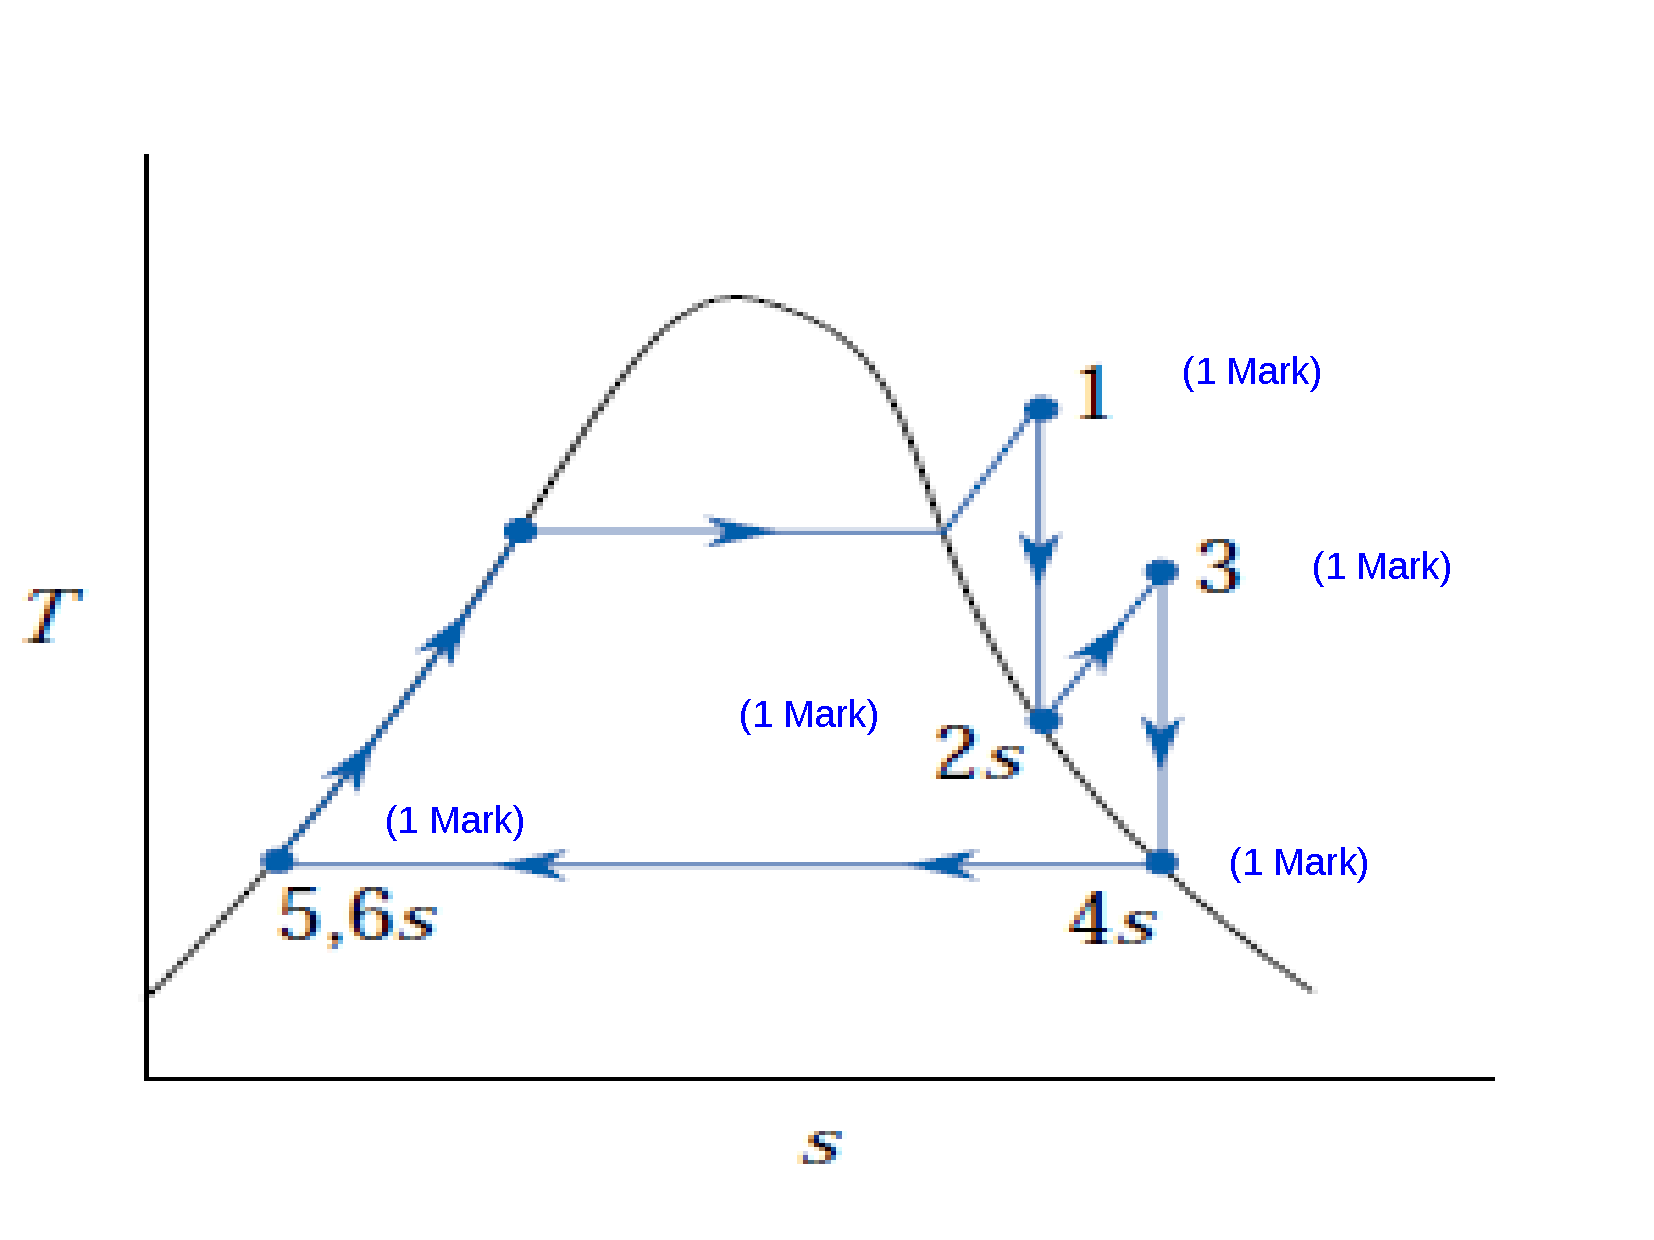
\includegraphics[width=12.cm,height=12cm,clip]{./Pics/Exam_Reheat_Rankine_Cycle3}
\end{center}
\end{figure}

\end{enumerate}

\clearpage

%%%
%%% Module 02
%%%
\item [Question 2:] \mbox{}\\
 
\begin{enumerate}[(a)]
\item 
\begin{displaymath}
421 \text{ billion kWh} = 421 \times 10^{12}  \text{ J.s}^{-1} \times 3600 \text{ s}  = 1.5 \times 10^{18} \text{ J of electricity.}
\end{displaymath}
Efficiencies of generation depend on turbine performance not on whether nuclear and or chemical fuels were used, so the electricity above must have been obtained from about: 
\begin{displaymath}
    \left(1.5 \times 10^{18} / 0.35\right) \text{ J of heat} =  4.3 \times 10^{18} \text{ J  of heat}
\end{displaymath}

If this had been raised from natural gas, the carbon dioxide release would have been: 
\begin{displaymath}                              
\left[ 4.3 \times 10^{18} \text{ J} / \left(889 × 103 \text{ J.mol}^{-1}\right)\right] \times 0.044 \text{ kg.mol}^{-1} \times 10^{-3} \text{ tonne.kg}^{-1} = 213 \text{ million tonnes}
\end{displaymath}

\item A supertanker, carrying 1 million barrels of oil, would if it blew up have a blast equivalent to that from the atomic bomb at Hiroshima. A blast of this magnitude was actually observed at a refinery fire in Venezuela in 2012 (either of these). 

\item Rate  of supply of coke = $\left[ 300 \times 10^{6}  \text{ J. s}^{-1} / \left( 25 \times 10^{6} \text{ J.kg}^{-1}\right)\right]  = 12 \text{ kg.s}^{-1}$\\ 
 rate of production of carbon dioxide = $12 \text{ kg.s}^{-1} \times \left( 44 / 12\right) \times 7 \times 24 \times 3600 \times 0.001 \text{ tonne per week}$ = $26611$ tonne per week. \\

For 10$\%$ mitigation of the carbon  10$\%$ of the heat must come from the citrus peel.\\
$10.8 \text{ kg.s}^{-1} \text{ of coke plus:}$ \\
$\left( 1.2 \times 25/7\right) \text{ kg.s}^{-1} \text{ of citrus peel} = 4.3 \text{ kg.s}^{-1} \text{ of citrus peel}$ \\ 
Ratio coke to citrus peel = $\left(10.8 / 4.3\right) = 2.5$ 

\item Suppliers are monitored by the Forest Stewardship Council (FSC) for replacement of trees felled with new plantings.

\end{enumerate}

\clearpage

%%%
%%% Module 03
%%%
\item [Question 3:]


\begin{itemize}
\item[(a)] The inlet has circumference $1$\,m. Therefore the radius of the inlet $r_1 = 1 / 2\pi = 0.15915$\,m and the area of the inlet $A_1 = \pi r_1^2 = 0.07958$\,m$^2$.\\
Similarly the outlet has circumference $0.6$\,m. Therefore the radius of the outlet $r_2 = 0.6/ 2\pi = 0.09549$\,m and the area of the outlet $A_2 = \pi r_2^2 = 0.02865$\,m$^2$.  \hfill \textbf{[1 Mark of 4]}


Evaluating the mass flux at the inlet gives
\begin{align*}
 \rho_1 = \frac{\dot{m}}{u_1 A_1} = \frac{4\,\mbox{kg\,s}^{-1}}{30\,\mbox{m\,s}^{-1} \times 0.07958\,\mbox{m}^2} = 1.6755\,\mbox{kg\,m}^{-3}.
\end{align*} \hfill \textbf{[1 Mark of 4]}

Rearranging the SFEE to give the gas velocity at the outlet implies
\begin{align*}
 u_2^2 = u_1^2 + \frac{2\left(\dot{Q} - \dot{W}_s\right)}{\dot{m}} + 2\left(h_1 - h_2\right).
\end{align*}
Therefore
\begin{align*}
 u_2^2 =& 30^2 + \frac{2\left(-15000 - 30000\right)}{4} + 2\left(70000 - 40000\right) \nonumber \\
 =& 900 - 22500 + 60000 \nonumber \\
 =& 38400\,\mbox{m}^2\,\mbox{s}^{-2},
\end{align*}
giving a fluid velocity at the outlet of
\begin{align*}
 u_2 =& 195.959\,\mbox{m\,s}^{-1}
\end{align*} \hfill \textbf{[1 Mark of 4]}

Now the gas density at the outlet can be calculated from the mass flux
\begin{align*}
 \rho_2 = \frac{\dot{m}}{u_2 A_2} = \frac{4\,\mbox{kg\,s}^{-1}}{195.959\,\mbox{m\,s}^{-1} \times 0.02865\,\mbox{m}^2} = 0.7125\,\mbox{kg\,m}^{-3}.
\end{align*} 

Finally the difference in gas density the turbine is given by
\begin{align*}
 \Delta \rho = \rho_1 - \rho_2 = 1.6755 - 0.7125 = 0.9630 \,\mbox{kg\,m}^{-3}.
\end{align*} \hfill \textbf{[1 Mark of 4]}

\item[(b)] The differential forms of for mass and energy conservation are
\begin{align*}
 \frac{\d{V}}{V} - \frac{\d{u}}{u} - \frac{\d{A}}{A} =& 0, \\
 \d{h} + u \, \d{u} =& 0.
\end{align*} \hfill \textbf{[1 Mark of 2]} \\
Eliminating $\d{u}$ between these two expressions gives
\begin{align*}
 \frac{\d{V}}{V} + \frac{\d{h}}{u^2} - \frac{\d{A}}{A} =& 0
\end{align*} \hfill \textbf{[1 Mark of 2]}

The speed of sound is the distance travelled during a unit of time by a sound wave propagating through a compressible medium. The Mach number is the non-dimensional ratio of the speed of a body moving through a fluid to the local speed of sound. For an isentropic process, the speed of sound is given by
\begin{align*}
 c = \left(\fracp{p}{\rho}\right)^{1/2},
\end{align*}
while the Mach number is defined to be
\begin{align*}
 \Ma = \frac{u}{c},
\end{align*} \hfill \textbf{[4 Marks]}

For an isentropic process the specific volume $V = 1/\rho$, is a function of just pressure and therefore satisfies
\begin{align*}
 \d{V} = \fracd{V}{p} \d{p}.
\end{align*}
In this expression the derivative can be written in terms of the speed of sound $c$ since
\begin{align*}
 \fracd{V}{p} = \fracp{V}{\rho} \fracp{\rho}{p} = -\frac{V^2}{c^2},
\end{align*}
and therefore
\begin{align*}
 \d{V} = -\frac{V^2}{c^2} \d{p}.
\end{align*} \hfill \textbf{[2 Marks of 3]}

For a general thermodynamic process
\begin{align*}
 \d{h} = T\,\d{s} + V \, \d{p}.
\end{align*}
However for an isentropic process the entropy remains constant $\d{s} = 0$, and the enthalpy is a function of just pressure. Changes in enthalpy are not related to changes in entropy, and
\begin{align*}
 \d{h} = V \, \d{p}.
\end{align*} \hfill \textbf{[1 Mark of 3]}

Hence if we eliminate $\d{V}$ and $\d{h}$,
\begin{align*}
 -\frac{V}{c^2} \d{p} + \frac{V}{u^2} \d{p} - \frac{\d{A}}{A} =& 0.
\end{align*}
Collecting together terms involving $\d{p}$ gives
\begin{align*}
 \frac{\d{A}}{A} = \left(\frac{V}{u^2} - \frac{V}{c^2}\right) \d{p} = \frac{V}{u^2}\left(1 - \frac{u^2}{c^2}\right) \d{p}.
\end{align*}
Given the definition of Mach number
\begin{align*}
 \frac{\d{A}}{A} = \frac{V}{u^2}\left(1 - \Ma^2\right) \d{p}.
\end{align*}
For an isentropic process the speed of sound can be used to eliminate $\d{p}$, giving
\begin{align*}
 \frac{\d{A}}{A} = \frac{V}{u^2}\left(1 - \Ma^2\right) c^2 \d{\rho}.
\end{align*}
Rearranging and using the definition of Mach number and specific density gives
\begin{align*}
 \frac{1}{\left(1 - \Ma^2\right) A} \d{A} = \frac{1}{\rho \Ma^2} \d{\rho}.
\end{align*}
If we're interested in changes along a pipe whose length is parameterized by $x$, then
\begin{align*}
 \frac{1}{\left(1 - \Ma^2\right) A} \fracd{A}{x} = \frac{1}{\rho \Ma^2} \fracd{\rho}{x},
\end{align*}
as required. \hfill \textbf{[5 Marks]}

For a supersonic diffuser $\left(1 - \Ma^2\right) < 0$, while $\fracd{A}{x} > 0$, $A>0$, $\rho>0$ and $\Ma^2>0$. Therefore $\fracd{\rho}{x} < 0$ and the gas density falls as gas flows along a supersonic diffuser. \hfill \textbf{[2 Marks]}
\end{itemize}

\clearpage


%%%
%%% Module 04
%%%
\item [Question 4:] Figure \ref{exam_refrig1} shows the $Ts$ diagram for the refrigeration cycle.

\begin{figure}[h]
\begin{center}
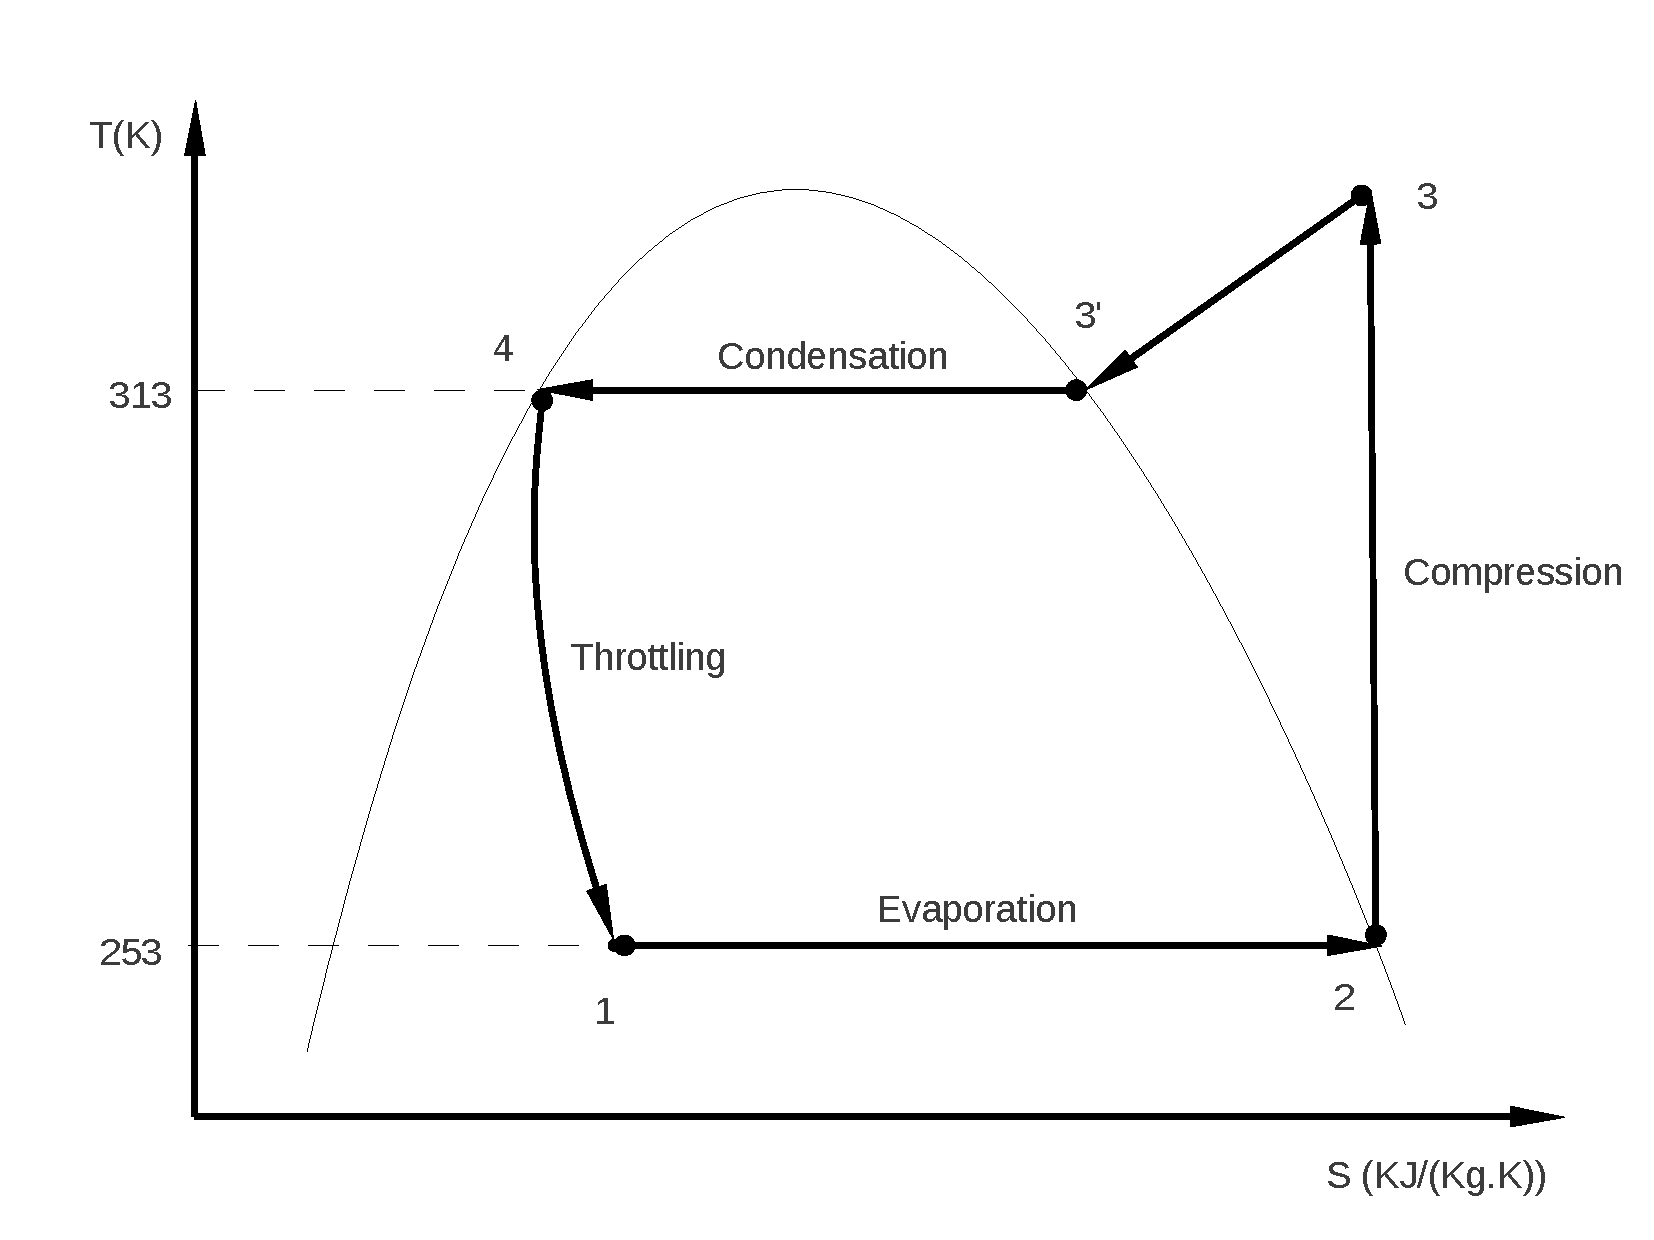
\includegraphics[width=10.cm,clip]{./Pics/Exam_Refrigeration1}
\caption{ Refrigeration cycle -- Question 4}
\label{exam_refrig1}
\end{center}
\end{figure}


\begin{figure}[h]
\begin{center}
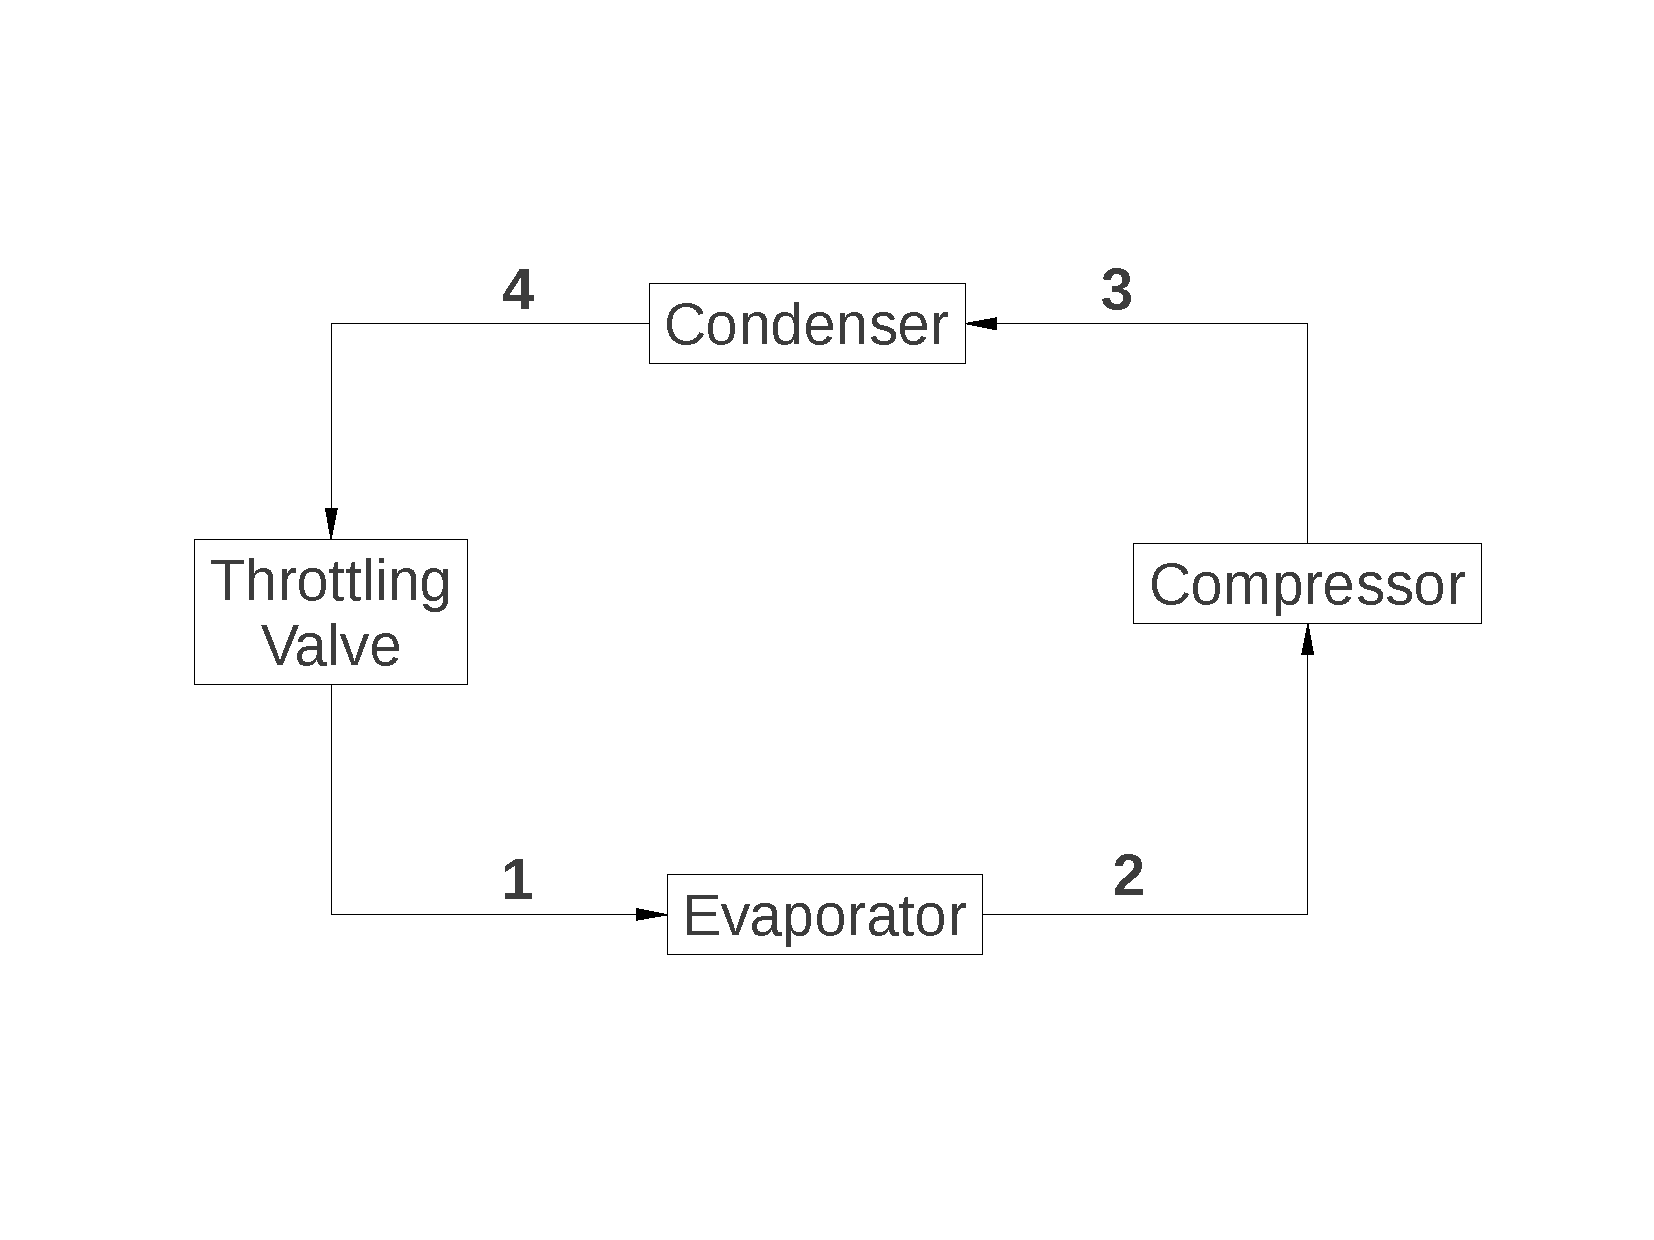
\includegraphics[width=10.cm,clip]{./Pics/Exam_Refrigeration2}
\caption{ Sketch of the vapour-compressed refrigeration -- Question 4.}
\label{exam_refrig2}
\end{center}
\end{figure}

Before solve the vapour-compressed refrigeration problem we should sketch the cycle (Fig. \ref{exam_refrig2} -- \textcolor{blue}{(1 Mark)}), and calculate the enthaplies (and entropies) of the the different stages of the cycle based on the data obtained from the thermodynamic table (for Freon-12),
\begin{center}
\begin{tabular}{|c c| c c c c c c| }
\hline
$T$             & $P_{s}$  & $V_{g}$  & $H_{f}$  & $H_{g}$   &  $S_{f}$   &  $S_{g}$   & {\it Specific Heat} \\
($^{\text{o}}$C)  & (bar)   & $\left(\text{m}^{3}/\text{kg}\right)$ & (kJ/kg) & (kJ/kg) & (kJ/(kg.K)) &  (kJ/(kg.K)) &   (kJ/(kg.K)) \\
\hline
-20   & 1.509 & 0.1088 & 17.8 & 178.61 & 0.073 & 0.7082 & -- \\
40    & 9.607 & --     & 74.53 & 203.05 & 0.2716 & 0.682 & 0.747 \\
\hline
\end{tabular}
\end{center}

\begin{description}
%
\item [Stage 2:] At $P_{2}=1.509\;bar$,
\begin{eqnarray}
&&\textcolor{red}{H_{2}=178.61\frc{kJ}{kg}}\;\;=H_{g}\;\;\;\textcolor{blue}{(1 Mark)} \nonumber \\
&&S_{2}=S_{g}=0.7082 \frc{kJ}{kg.K} \nonumber 
\end{eqnarray}

%
\item [Stage 3:] The refrigerant fluid undertakes an \underline{isentropic compression} $\left(S_{3}=S_{2}\right)$ leading to a superheated fluid. Because we do not have the full saturation tables we need to use fundamental relationship to calculate the properties of the superheated fluid,
\begin{displaymath}
H_{3} = H_{3}^{\text{sat}}+C_{p}\left(T_{3}-T_{3}^{sat}\right)
\end{displaymath} 
where $T_{3}^{\text{sat}}=T^{\text{sat}}\left(P=9.607\;bar\right)=40^{\text{o}}\text{C}=313.15\;\text{K}$. However we first need to calculate the temperature, $T_{3}$, of the superheated fluid,
\begin{eqnarray}
&&S_{3} = 0.7082 = S_{3}^{\text{sat}} + C_{p}\ln\left(\frc{T_{3}}{T_{3}^{\text{sat}}}\right) = 0.682 + 0.747 \ln\left(\frc{T_{3}}{313.15}\right) \nonumber \\
&&\Longrightarrow \;\; \textcolor{red}{T_{3}= 324.33 K} \;\textcolor{blue}{(1\; Mark)} \nonumber
\end{eqnarray}
Now, replacing $T_{3}$ in the above equation for $H_{3}$,
\begin{displaymath}
\textcolor{red}{H_{3}}=H_{3}^{\text{sat}}+C_{p}\left(T_{3}-T_{3}^{\text{sat}}\right)=203.05+0.747\left(324.33-313.15\right)=\textcolor{red}{211.40\frc{kJ}{kg}}\;\textcolor{blue}{(1\; Mark)}
\end{displaymath}
%
\item [Stage 4:] Saturated liquid at the exit of the condenser $\left(P_{4}=9.607\; bar\right) \Longrightarrow\; \textcolor{red}{H_{4}}=H_{f}=\textcolor{red}{74.5\frc{kJ}{kg}}$ \textcolor{blue}{(1\; Mark)}. 

%
\item [Stage 1:] Isenthalpic expansion through the throttling valve, $\textcolor{red}{H_{1}}=H_{4}=\textcolor{red}{74.5\frc{kJ}{kg}}$ \textcolor{blue}{(1\; Mark)}. 
%
\end{description}
Now that we have all key-parameters, 

\begin{enumerate}[(a)]
\item The power required by the compressor is
\begin{displaymath}
\mathcal{P}=\dot{m}_{r}\left(H_{3}-H_{2}\right)
\end{displaymath}
where $\dot{m}_{r}$ is the mass flow rate of the refrigerant fluid that can be calculated with the help of the given refrigerant capacity, $R_{n}$,
\begin{eqnarray}
R_{n} = 20 = \dot{m}_{r}\left(H_{2}-H_{1}\right) =  \dot{m}_{r}\left(178.61-74.53\right) \; \Longrightarrow \; \textcolor{red}{\dot{m}_{r}=0.1922\frc{kg}{s}}\;\textcolor{blue}{(1\; Mark)} \nonumber
\end{eqnarray}
and 
\begin{displaymath}
\mathcal{P}=0.1922\left(211.40-178.61\right)\; \Longrightarrow \; \textcolor{red}{\mathcal{P}}= 6.3022\frc{kJ}{s}=\textcolor{red}{6302.2\;W}\;\textcolor{blue}{(3\; Mark)}
\end{displaymath}

\item In order to determine the piston displacement in the cylinder, we first need to calculate the volumetric efficiency given by
\begin{displaymath}
\textcolor{red}{\eta_{\text{vol}}} = 1 + C - C\left(\frc{P_{d}}{P_{s}}\right)^{1/n} = 1 + 0.03 - 0.03\left( \frc{9.607}{1.509}\right)^{1/1.13}=\textcolor{red}{0.876} \;\;\textcolor{blue}{(2\; Mark)}
\end{displaymath}

The volume of the fluid at intake conditions is,
\begin{displaymath}
\textcolor{red}{\dot{V}_{r}}=\dot{m}_{r}V_{g}=0.1922 \times 0.1088 = \textcolor{red}{0.0209\frc{m^{3}}{s}} \;\;\textcolor{blue}{(2\; Mark)}
\end{displaymath}

The swept volume rate is,
\begin{displaymath}
\textcolor{red}{\dot{V}_{\text{swept}}} = \frc{\dot{V}_{r}}{\eta_{\text{vol}}} = \frc{0.0209}{0.876} = \textcolor{red}{2.385\times 10^{-2}\frc{m^{3}}{s}} \;\;\textcolor{blue}{(2\; Mark)}
\end{displaymath}

The piston operates at {\it 300 rpm}, thus each stroke is completed in $t_{r}$,
\begin{eqnarray}
300 \;\text{rotations} \;\; &\uline{0.5cm}& \;\;1\;\text{min}=60\;\text{sec} \nonumber\\
1 \;\text{rotation} \;\; &\uline{0.5cm}& \;\; t_{r} \nonumber\\
\end{eqnarray}
\textcolor{red}{$t_{r}=0.2\text{ s }$} \textcolor{blue}{(2\; Mark)}. Thus, it takes {\it 0.2 seconds} to fill up the cylinder with {\it Freon} in the compressor operating with a reciprocating (or piston) engine. Now calculating the piston displacement -- $V_{\text{swept}}$,
\begin{eqnarray}
2.385\times 10^{-2} m^{3} \;\; &\uline{0.5cm}& \;\; 1\;\text{s} \nonumber \\
V_{\text{swept}}                &\uline{0.5cm}& 0.2\;\text{s} \nonumber
\end{eqnarray}

\textcolor{red}{$V_{\text{swept}}=4.771\times 10^{-3}\;m^{3}$} \textcolor{blue}{(2\; Mark)}

\end{enumerate}
\clearpage

%%%
%%% Module 05
%%%
\item [Question 5:] 

The specific humidity $\omega$ is the ratio of the mass of water vapour $m_v$, to the mass of dry air $m_a$ and satisfies the equation
\begin{align*}
 \omega = \frac{m_v}{m_a}.
\end{align*}
As both water vapour and dry air behave like ideal gases, in some arbitrary volume $V$,
\begin{align*}
 \omega = \frac{m_v}{m_a} = \frac{\rho_v}{\rho_a} = \frac{p_v}{R_v T} \frac{R_a T}{p_a} = \frac{R_a p_v}{R_v p_a}.
\end{align*}
The ratio of specific gas constants $R_a/R_v = 0.622$, while the partial pressures of dry air and water vapour satisfy $p_a = p - p_v$. Hence
\begin{align*}
 \omega = \frac{0.622 p_v}{p - p_v}.
\end{align*} \hfill \textbf{[4 Marks]}

The saturation pressure of water
\begin{align*} 
 p_g = \phi p_v.
\end{align*}
Hence eliminating $p_v$ from the previous expression gives
\begin{align*}
 \omega = \frac{0.622 \phi p_g}{p - \phi p_g}.
\end{align*} \hfill \textbf{[2 Marks]}


The heating and humidification are split into two steady process. Firstly a heater (with inlet properties labelled 1 and outlet properties labelled 2) and secondly a humidifier (with inlet properties labelled 2 and outlet properties labelled 3).

\begin{itemize}
\item[(a)] The partial vapour pressure at the inlet 1, is
\begin{align*}
 p_{v_1} = \phi_1 p_{g_1} = \phi p_\text{sat @ 10$^\circ$C} = 0.25 \times 1.4028\,\mbox{kPa} = 0.3507\,\mbox{kPa}.
\end{align*} \hfill \textbf{[1 Mark]} \\
Hence the partial pressure of dry air is given by
\begin{align*}
 p_{a_1} = p_1 - p_{v_1} = 100\,\mbox{kPa} - 0.3507\,\mbox{kPa} = 99.6493\,\mbox{kPa}.
\end{align*} \hfill \textbf{[1 Mark]} \\
The specific humidity is given by
\begin{align*}
 \omega_1 = \frac{0.622 p_{v_1}}{p_1 - p_{v_1}} = \frac{0.622 \times 0.3507\,\mbox{kPa}}{100\,\mbox{kPa} - 0.3507\,\mbox{kPa}} = 0.00219\,\mbox{kg H$_2$O/ kg dry air}.
\end{align*} \hfill \textbf{[1 Mark]} \\

\item[(b)] Applying the mass and energy balances on the heating section gives
\begin{align*}
 \mbox{Dry air mass balance:} &~~~~~ \dot{m}_{a_1} = \dot{m}_{a_2} = \dot{m}_a, \\
 \mbox{Water mass balance:} &~~~~~ \dot{m}_{a_1} \omega_1 = \dot{m}_{a_2} \omega_2, ~~ \Rightarrow ~~ \omega_1 = \omega_2, \\
 \mbox{Energy balance:} &~~~~~ \dot{Q} = \dot{m}_a h_2 - \dot{m}_a h_1.
\end{align*} \hfill \textbf{[2 Marks]}

The total specific enthalpy at 1, the inlet is
\begin{align*}
 h_1 = c_p T_1 + \omega_1 h_{g_1} =& \left(1.005\,\mbox{kJ/(kg\,K)} \times \left(12 + 173.15\right)\,\mbox{K}\right) \nonumber \\
 &+ \left(0.00219 \times 2523\,\mbox{kJ/kg}\right) \nonumber \\
 =& 292.0988\,\mbox{kJ/kg}.
\end{align*}
The total specific enthalpy at 2, the outlet of the heating is
\begin{align*}
 h_2 = c_p T_2 + \underbrace{\omega_2}_{=\omega_1} h_{g_2} =& \left(1.005\,\mbox{kJ/(kg\,K)} \times \left(20 + 173.15\right)\,\mbox{K}\right) \nonumber \\
 &+ \left(0.00219 \times 2537\,\mbox{kJ/kg}\right) \nonumber \\
 =& 300.1693\,\mbox{kJ/kg}
\end{align*} \hfill \textbf{[2 Marks]}

The specific volume of dry air at 1, is given by
\begin{align*}
 V_1 = \frac{R_a T_1}{p_{a_1}} = \frac{287.058\,\mbox{J/(kg\,K)} \left(12 + 273.15\right)\,\mbox{K}}{99649.3\,\mbox{Pa}} = 0.8215\,\mbox{m}^3\mbox{/kg}.
\end{align*}
Therefore the mass flux of dry air through the inlet
\begin{align*}
 \dot{m}_a = \frac{q_1}{V_1} = \frac{40\,\mbox{m}^3\mbox{/min}}{0.8185\,\mbox{m}^3\mbox{/kg}} = 48.6886\,\mbox{kg/min},
\end{align*}
where $q_1 = 40$\,m$^3$/min is the total volume flux through the inlet. \hfill \textbf{[1 Mark]}

Hence the energy conservation equation gives the rate at which heat is transferred to the air
\begin{align*}
 \dot{Q} = \dot{m}_a \left(h_2 - h_1\right) = 48.6958\,\mbox{kg/min} \left(300.1693\,\mbox{kJ/kg} - 292.0988\,\mbox{kJ/kg}\right) = 392.9488\,\mbox{kJ/min}.
\end{align*} \hfill \textbf{[1 Mark]}


\item[(c)] The mass balance for water in the humidifying section can be expressed as
\begin{align*}
 \dot{m}_{a_2} \omega_2 + \dot{m}_w = \dot{m}_{a_3} \omega_3,
\end{align*}
or
\begin{align*}
 \dot{m}_w = \dot{m}_a \left(\omega_3 - \omega_2\right).
\end{align*} \hfill \textbf{[2 Marks]} \\
Here $\omega_2 = \omega_1$, while the specific humidity at 3, the outlet is given by
\begin{align*}
 \omega_3 = \frac{0.622 \phi_3 p_{g_3}}{p_3 - \phi_3 p_{g_3}} = \frac{0.622 \times 0.55 \times 2.9858}{100 - \left(0.55 \times 2.9858\right)} = 0.0104\,\mbox{kg H$_2$O/ kg dry air}.
\end{align*} \hfill \textbf{[1 Mark]} \\
Therefore the required mass flow rate of steam is
\begin{align*}
 \dot{m}_w = \dot{m}_a \left(\omega_3 - \omega_2\right) = 48.6886\,\mbox{kg/min}\left(0.0104 - 0.00219\right) = 0.3990\,\mbox{kg/min}
\end{align*} \hfill \textbf{[2 Marks]}

\end{itemize}




\end{description}

%\begin{Large}
%\include{Module_Questions}
%% Aberdeen style guide should be followed when using this
% layout. Their template powerpoint slide is used to extract the
% Aberdeen color and logo but is otherwise ignored (it has little or
% no formatting in it anyway).
%
% http://www.abdn.ac.uk/documents/style-guide.pdf

%%%%%%%%%%%%%%%%%%%% Document Class Settings %%%%%%%%%%%%%%%%%%%%%%%%%
% Pick if you want slides, or draft slides (no animations)
%%%%%%%%%%%%%%%%%%%%%%%%%%%%%%%%%%%%%%%%%%%%%%%%%%%%%%%%%%%%%%%%%%%%%%
%Normal document mode%
\documentclass[10pt,compress]{beamer}
%Draft or handout mode
%\documentclass[10pt,compress,handout]{beamer}
%\documentclass[10pt,compress,handout,ignorenonframetext]{beamer}

%%%%%%%%%%%%%%%%%%%% General Document settings %%%%%%%%%%%%%%%%%%%%%%%
% These settings must be set for each presentation
%%%%%%%%%%%%%%%%%%%%%%%%%%%%%%%%%%%%%%%%%%%%%%%%%%%%%%%%%%%%%%%%%%%%%%
\newcommand{\shortname}{jefferson.gomes@abdn.ac.uk}
\newcommand{\fullname}{Dr Jeff Gomes}
\institute{School of Engineering}
\newcommand{\emailaddress}{}%jefferson.gomes@abdn.ac.uk}
\newcommand{\logoimage}{../../FigBanner/UoAHorizBanner}
\title{Chemical Thermodynamics (EG3029)}
\subtitle{Module 3: Volumetric Properties of Pure Fluids}
\date[2014-15]{2014-15}

%%%%%%%%%%%%%%%%%%%% Template settings %%%%%%%%%%%%%%%%%%%%%%%%%%%%%%%
% You shouldn't have to change below this line, unless you want to.
%%%%%%%%%%%%%%%%%%%%%%%%%%%%%%%%%%%%%%%%%%%%%%%%%%%%%%%%%%%%%%%%%%%%%%
\usecolortheme{whale}
\useoutertheme{infolines}

% Use the fading effect for items that are covered on the current
% slide.
\beamertemplatetransparentcovered

% We abuse the author command to place all of the slide information on
% the title page.
\author[\shortname]{%
  \fullname\\\ttfamily{\emailaddress}
}


%At the start of every section, put a slide indicating the contents of the current section.
\AtBeginSection[] {
  \begin{frame}
    \frametitle{Section Outline}
    \tableofcontents[currentsection]
  \end{frame}
}

% Allow the inclusion of movies into the Presentation! At present,
% only the Okular program is capable of playing the movies *IN* the
% presentation.
\usepackage{multimedia}
\usepackage{animate}

%% Handsout -- comment out the lines below to create handstout with 4 slides in a page with space for comments
\usepackage{handoutWithNotes}
%\pgfpagesuselayout{2 on 1 with notes}[a4paper,border shrink=10mm]
%%%%% Color settings
\usepackage{color}
%% The background color for code listings (i.e. example programs)
\definecolor{lbcolor}{rgb}{0.9,0.9,0.9}%
\definecolor{UoARed}{rgb}{0.64706, 0.0, 0.12941}
\definecolor{UoALight}{rgb}{0.85, 0.85, 0.85}
\definecolor{UoALighter}{rgb}{0.92, 0.92, 0.92}
\setbeamercolor{structure}{fg=UoARed} % General background and higlight color
\setbeamercolor{frametitle}{bg=black} % General color
\setbeamercolor{frametitle right}{bg=black} % General color
\setbeamercolor{block body}{bg=UoALighter} % For blocks
\setbeamercolor{structure}{bg=UoALight} % For blocks
% Rounded boxes for blocks
\setbeamertemplate{blocks}[rounded]

%%%%% Font settings
% Aberdeen requires the use of Arial in slides. We can use the
% Helvetica font as its widely available like so
% \usepackage{helvet}
% \renewcommand{\familydefault}{\sfdefault}
% But beamer already uses a sans font, so we will stick with that.

% The size of the font used for the code listings.
\newcommand{\goodsize}{\fontsize{6}{7}\selectfont}

% Extra math packages, symbols and colors. If you're using Latex you
% must be using it for formatting the math!
\usepackage{amscd,amssymb} \usepackage{amsfonts}
\usepackage[mathscr]{eucal} \usepackage{mathrsfs}
\usepackage{latexsym} \usepackage{amsmath} \usepackage{bm}
\usepackage{amsthm} \usepackage{textcomp} \usepackage{eurosym}
% This package provides \cancel{a} and \cancelto{a}{b} to "cancel"
% expressions in math.
\usepackage{cancel}

\usepackage{comment} 

% Get rid of font warnings as modern LaTaX installations have scalable
% fonts
\usepackage{type1cm} 

%\usepackage{enumitem} % continuous numbering throughout enumerate commands

% For exact placement of images/text on the cover page
\usepackage[absolute]{textpos}
\setlength{\TPHorizModule}{1mm}%sets the textpos unit
\setlength{\TPVertModule}{\TPHorizModule} 

% Source code formatting package
\usepackage{listings}%
\lstset{ backgroundcolor=\color{lbcolor}, tabsize=4,
  numberstyle=\tiny, rulecolor=, language=C++, basicstyle=\goodsize,
  upquote=true, aboveskip={1.5\baselineskip}, columns=fixed,
  showstringspaces=false, extendedchars=true, breaklines=false,
  prebreak = \raisebox{0ex}[0ex][0ex]{\ensuremath{\hookleftarrow}},
  frame=single, showtabs=false, showspaces=false,
  showstringspaces=false, identifierstyle=\ttfamily,
  keywordstyle=\color[rgb]{0,0,1},
  commentstyle=\color[rgb]{0.133,0.545,0.133},
  stringstyle=\color[rgb]{0.627,0.126,0.941}}

% Allows the inclusion of other PDF's into the final PDF. Great for
% attaching tutorial sheets etc.
\usepackage{pdfpages}
\setbeamercolor{background canvas}{bg=}  

% Remove foot note horizontal rules, they occupy too much space on the slide
\renewcommand{\footnoterule}{}

% Force the driver to fix the colors on PDF's which include mixed
% colorspaces and transparency.
\pdfpageattr {/Group << /S /Transparency /I true /CS /DeviceRGB>>}

% Include a graphics, reserve space for it but
% show it on the next frame.
% Parameters:
% #1 Which slide you want it on
% #2 Previous slides
% #3 Options to \includegraphics (optional)
% #4 Name of graphic
\newcommand{\reserveandshow}[4]{%
\phantom{\includegraphics<#2|handout:0>[#3]{#4}}%
\includegraphics<#1>[#3]{#4}%
}

\newcommand{\frc}{\displaystyle\frac}
\newcommand{\red}{\textcolor{red}}
\newcommand{\blue}{\textcolor{blue}}
\newcommand{\green}{\textcolor{green}}
\newcommand{\purple}{\textcolor{purple}}
 
\begin{document}

% Title page layout
\begin{frame}
  \titlepage
  \vfill%
  \begin{center}
    \includegraphics[clip,width=0.8\textwidth]{\logoimage}
  \end{center}
\end{frame}

% Table of contents
\frame{ \frametitle{Slides Outline}
  \tableofcontents
}


%%%%%%%%%%%%%%%%%%%% The Presentation Proper %%%%%%%%%%%%%%%%%%%%%%%%%
% Fill below this line with \begin{frame} commands! It's best to
% always add the fragile option incase you're going to use the
% verbatim environment.
%%%%%%%%%%%%%%%%%%%%%%%%%%%%%%%%%%%%%%%%%%%%%%%%%%%%%%%%%%%%%%%%%%%%%%


%%%
%%% SECTION
%%%
\section{General Remarks}

%%%
%%% Slides
%%%
\begin{frame}
 \frametitle{Aims and Objectives}
   \begin{enumerate}
     \item<1-> In Modules 1 and 2, we learnt:
       \begin{enumerate}
         \item<1-> the laws of Thermodynamics and how they describe thermal equilibrium of species in closed and opened systems.
         \item<1-> how to obtain and calculate relevant thermodynamics properties for chemical species.
         \item<1-> spontaneity of processes.
       \end{enumerate} 
     \item<2-> This Module focuses on 
         \begin{enumerate}
           \item<2-> PVT behaviour of pure chemical species in equilibrium,
           \item<2-> Equations of state commonly used in industry.
         \end{enumerate}
   \end{enumerate}

\end{frame}


%%%
%%% SECTION
%%%
\section{Bibliography}
\begin{frame}
 \frametitle{Suggested References}
  Literature relevant for this module:
  \begin{enumerate}[(a)]
   \item J.M. Smith, H.C. Van Ness, M.M. Abbott, $\lq$Introduction to Chemical Engineering Thermodynamics', 6$^{th}$ Edition: Chapter 3;
   \item Y.A. Cengel, M.A. Boles, $\lq$Thermodynamics -- An Engineering Approach', 5$^{th}$ Edition: Chapter 3; 
   \item M.J. Moran, H.N. Saphiro, D.D. Boettner, M.B. Bailey, $\lq$Principles of Engineering Thermodynamics', 7$^{th}$ Edition: Chapters 3;
   \item C. Borgnakke, R.E. Sonntag,$\lq$Fundamentals of Thermodynamics',8$^{th}$ Edition: Chapter 2.
  \end{enumerate}
\end{frame}



%%%
%%% SECTION
%%%
\section{PVT Behaviour of Pure Substances}

%%%
%%% SUBSECTION
%%%
\subsection{Phase Diagram and Gibbs Rule} 

%%%
%%% Slide
%%%
\scriptsize
\begin{frame}
 \frametitle{PT Diagram for Pure Substances}
  \begin{columns}
    \begin{column}[l]{0.5\linewidth}\scriptsize
      \begin{enumerate}[(a)]%\scriptsize
        \item <1-> Recall the Gibbs phase rule (Module 1):
           \visible<1->{\begin{displaymath}
             \Psi = 2 + \mathcal{C} - \mathcal{P}
           \end{displaymath}
             where $\Psi$ is the number of \textcolor{blue}{degrees of freedom} for the system, \textcolor{blue}{2} refers to the independent variables ($T$ and $P$), \textcolor{blue}{$\mathcal{C}$} is the number of chemical species and \textcolor{blue}{$\mathcal{P}$} is the number of phases;}   
        \item<2-> The \textcolor{blue}{$PT$ phase diagram} describes fluid behaviour and phase change; 
        \item<3-> For example: \textcolor{blue}{A}-\;-\;-\textcolor{red}{B} defines a phase transition from \textcolor{blue}{liquid} to \textcolor{red}{gas} regions without crossing the phase boundary (vaporisation);
        \item<4-> \textcolor{red}{However}, there is \textcolor{blue}{no} information about the volume in the {\it PT} diagram.
      \end{enumerate}
    \end{column}
    \begin{column}[l]{0.5\linewidth}\scriptsize
      \begin{figure}%
        \begin{center}
          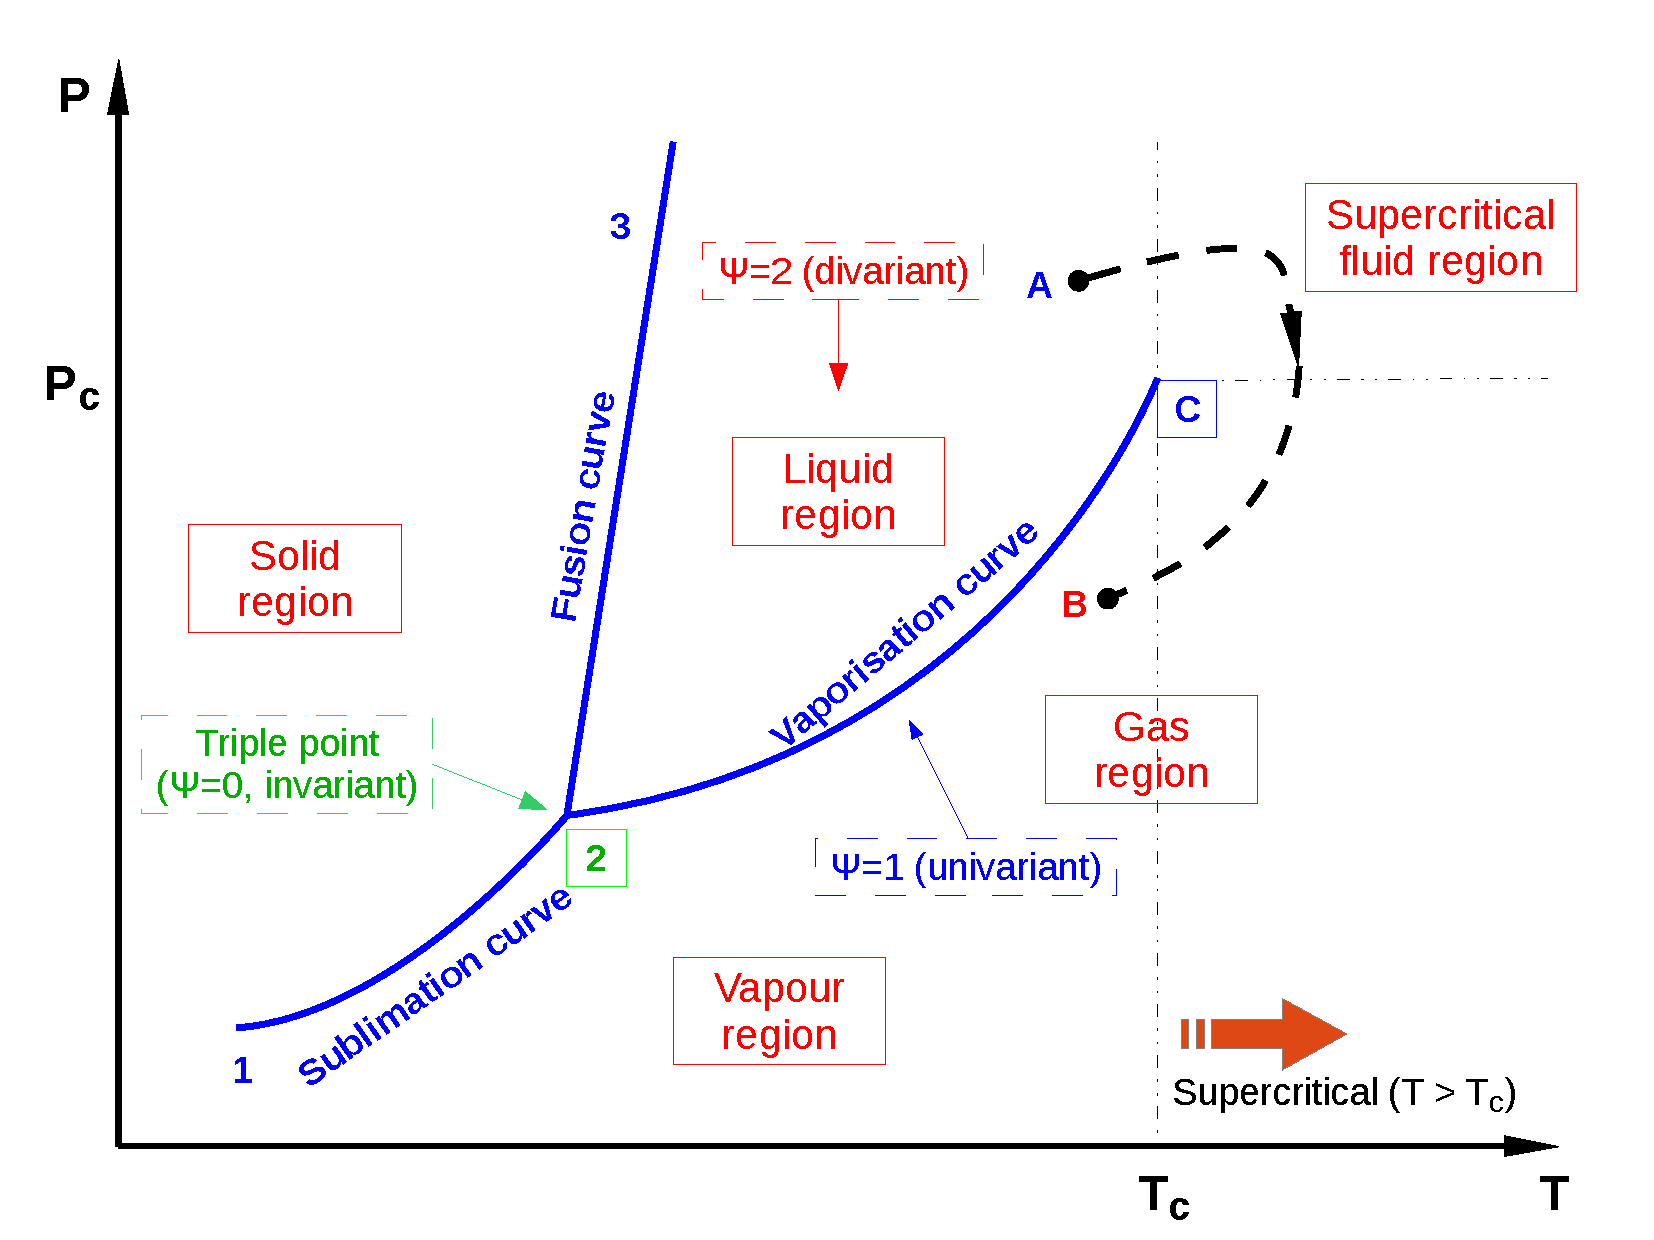
\includegraphics[width=1.05\columnwidth,clip]{./Pics/PT_Diagram}
        \end{center}
      \end{figure}
    \end{column}
  \end{columns}
\end{frame}
\normalsize



%%%
%%% Slide
%%%
\scriptsize
\begin{frame}
 \frametitle{PV Diagram}
  \begin{columns}
    \begin{column}[l]{0.5\linewidth}
      \visible<1->{\begin{figure}%
        \begin{center}
          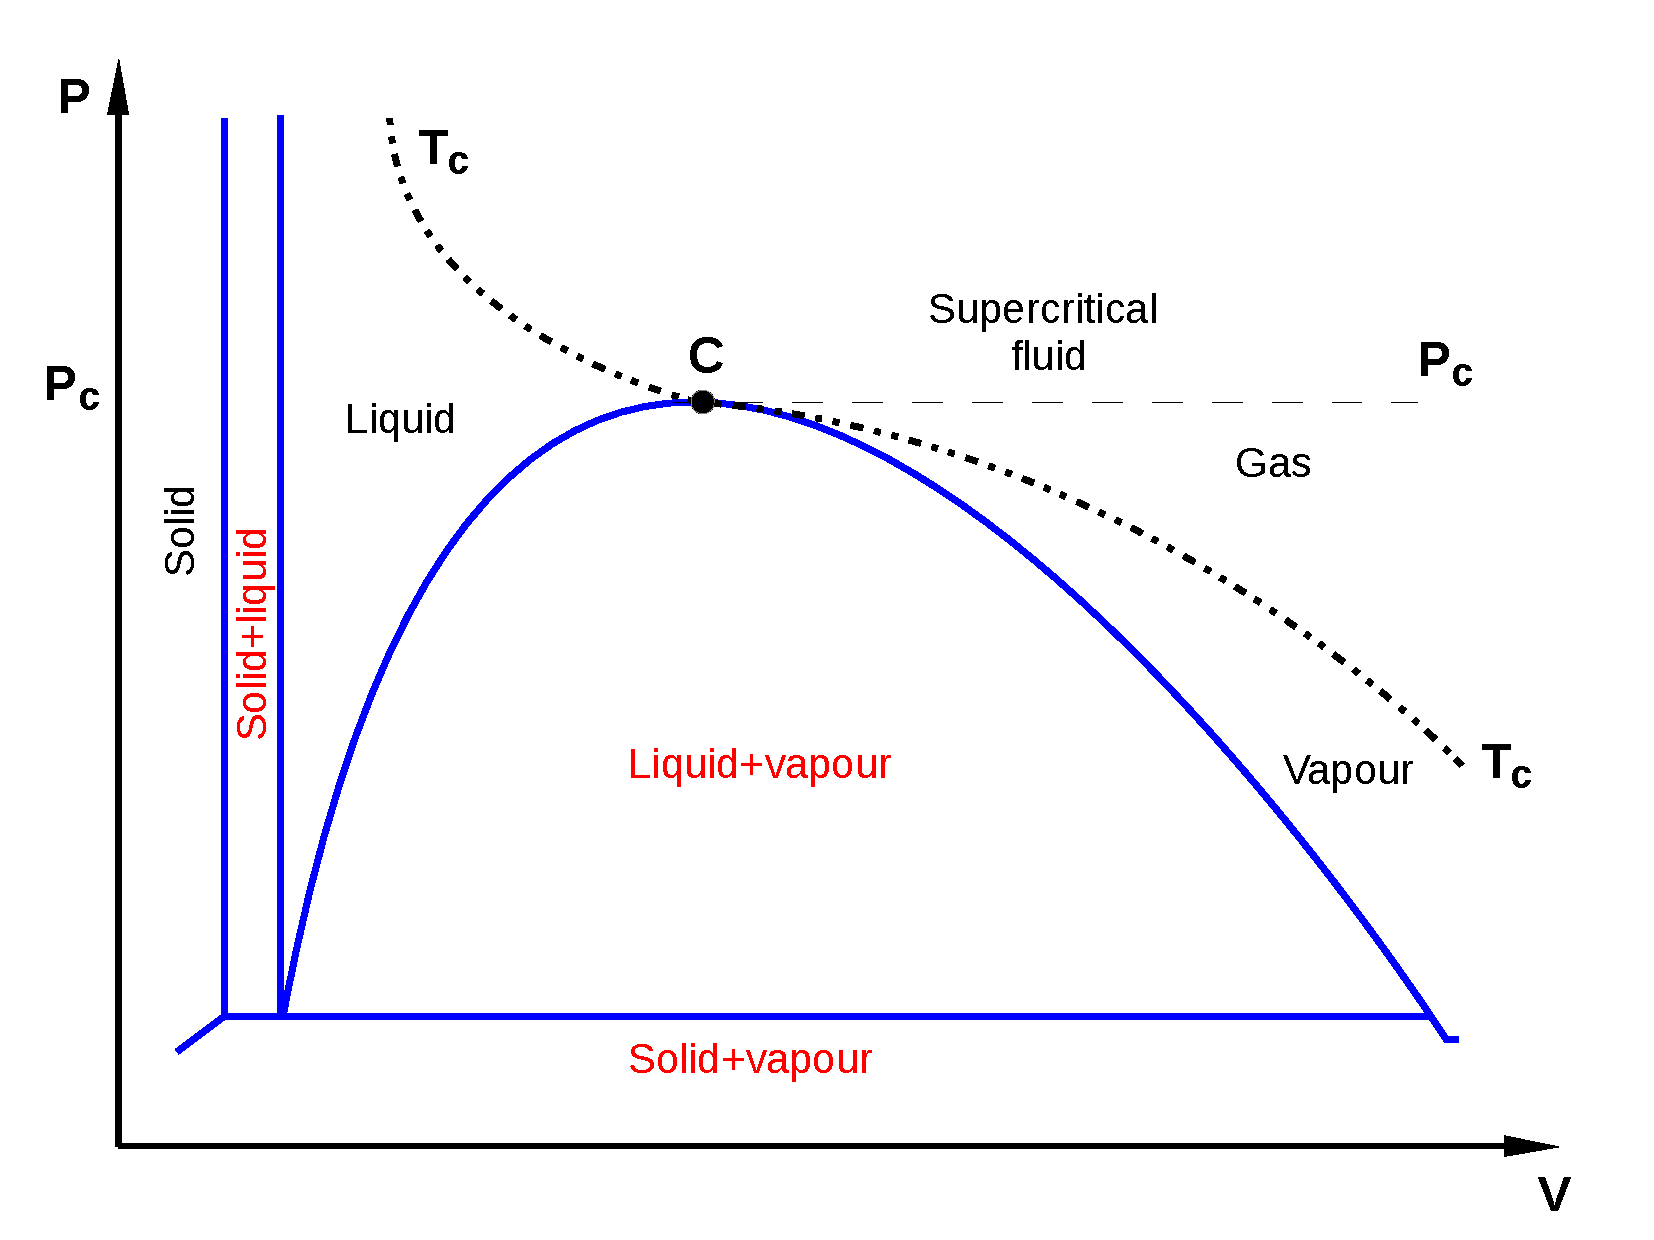
\includegraphics[width=\columnwidth,clip]{./Pics/PV_Diagram1}
        \end{center}
      \end{figure}}
      \begin{enumerate} \scriptsize
        \item<1-> Two-phase regions (e.g., liquid+vapor) are represented by \textcolor{red}{areas} and;
        \item<2-> Lines represent the actual transition transition between \textcolor{blue}{single phase} to \textcolor{blue}{two phases} regions, thus;
        \item<2-> The \textcolor{blue}{triple point} is the horizontal line between the 3 phases;
      \end{enumerate}
    \end{column}
    \begin{column}[l]{0.5\linewidth}\scriptsize
      \visible<3->{\begin{figure}%
        \begin{center}
          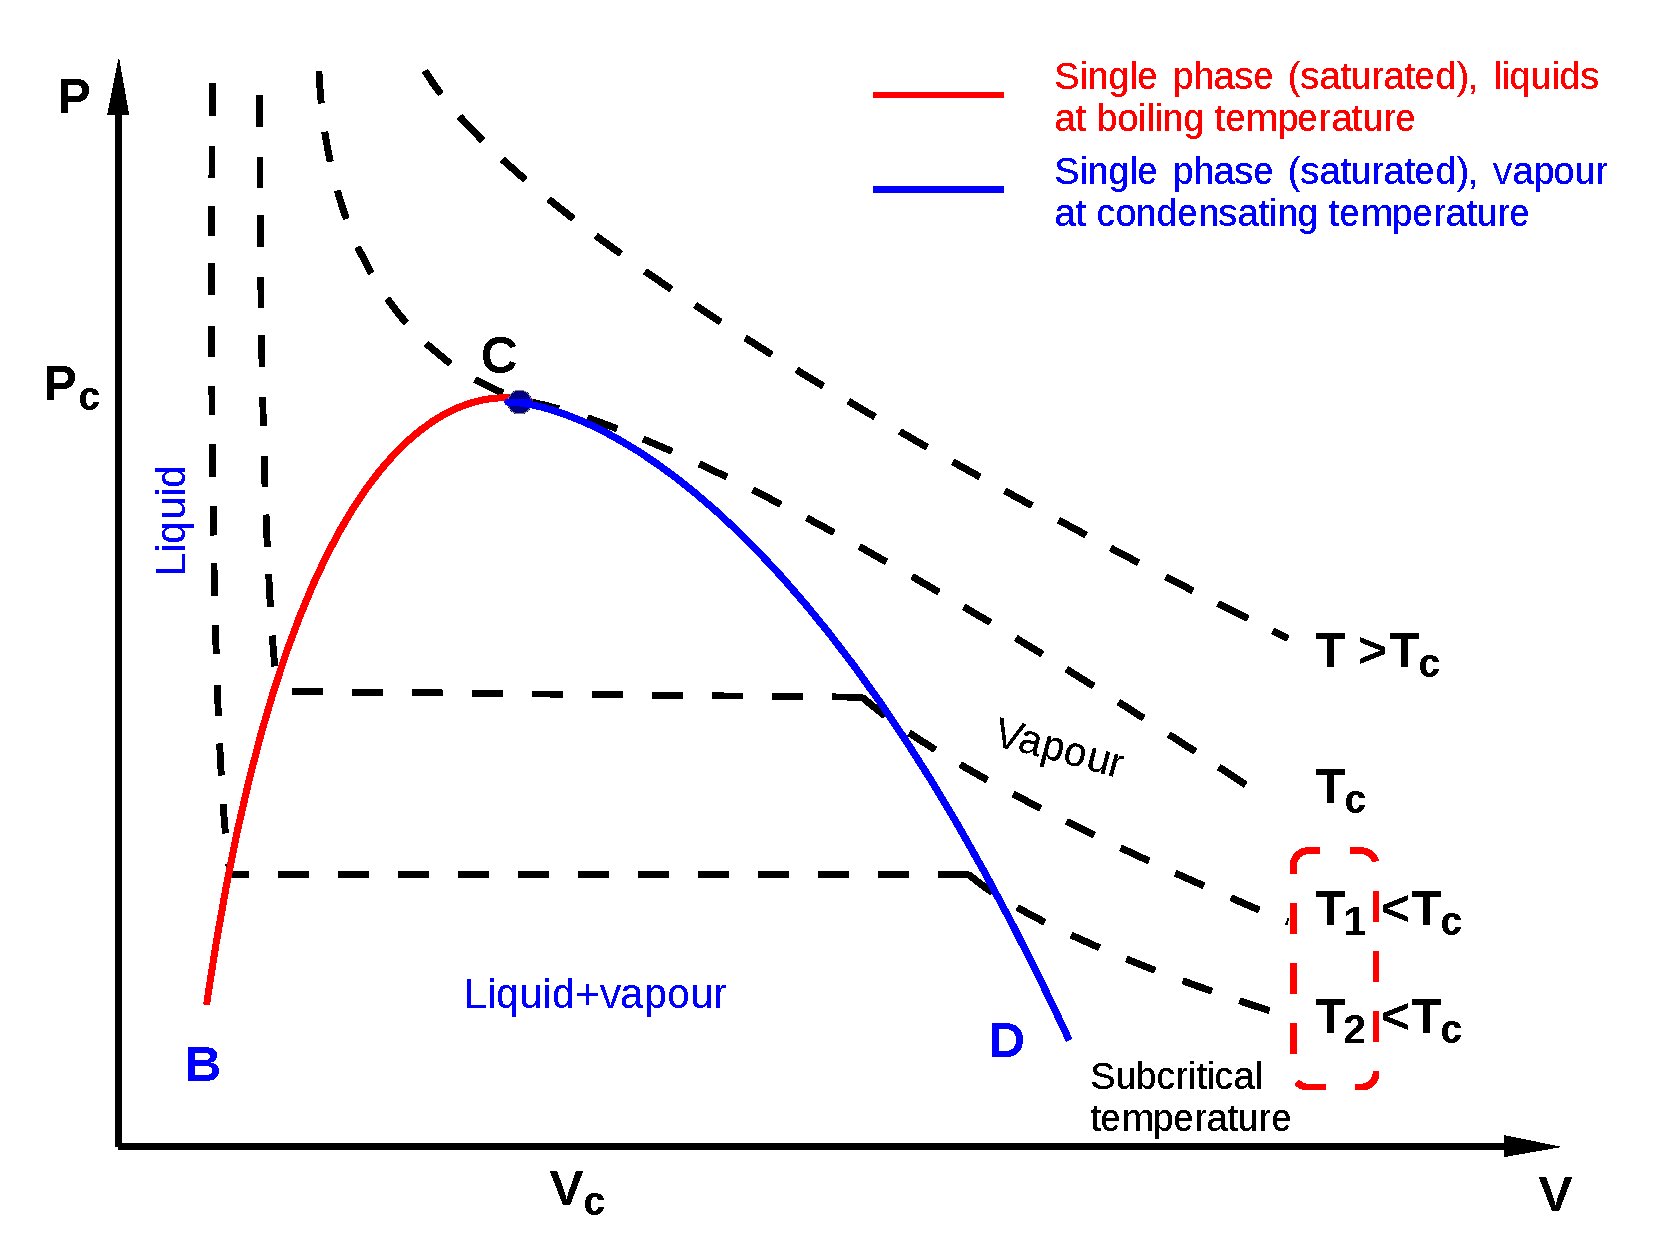
\includegraphics[width=\columnwidth,clip]{./Pics/PV_Diagram2}
        \end{center}
      \end{figure}}
      \begin{enumerate}\setcounter{enumi}{3}
        \item<3-> The isotherms range from \textcolor{blue}{subcooled liquid} to \textcolor{blue}{superheated vapor} regions; 
        \item<3-> Isotherms are \textcolor{red}{steep} in the \textcolor{blue}{subcooled liquid}  region because liquid volumes have little changes with large change in pressure.
      \end{enumerate}
    \end{column}
  \end{columns}
\end{frame}
\normalsize

%%%
%%% Slide
%%%
\scriptsize
\begin{frame}
 \frametitle{PV Diagram}
      \visible<1->{\begin{figure}%
        \begin{center}
          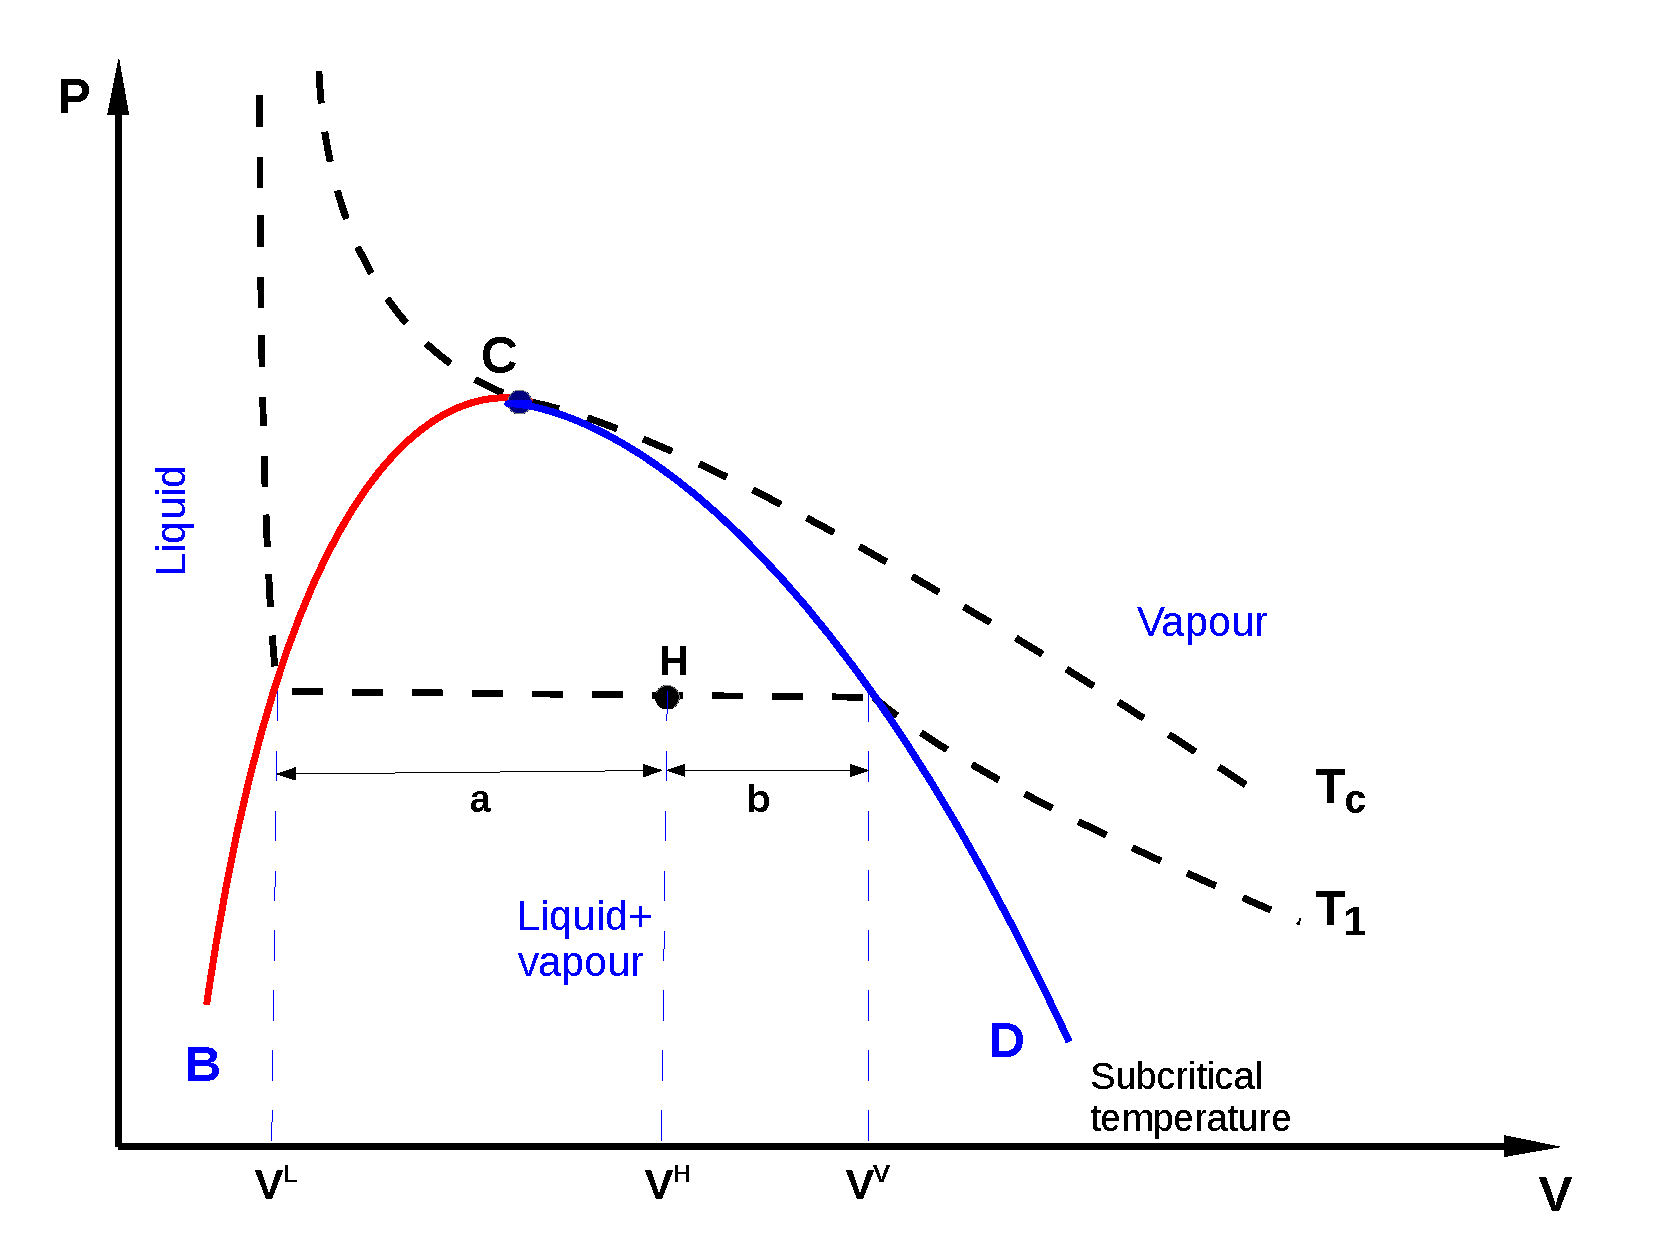
\includegraphics[width=.6\columnwidth,clip]{./Pics/PV_Diagram3}
        \end{center}
      \end{figure}}
      \visible<2->{\begin{displaymath}
         \frc{a}{b} = \frc{V^{H}-V^{L}}{V^{V}-V^{H}} = \frc{m^{V}}{m^{L}} = \frc{\text{mass of saturated vapour}}{\text{mass of saturated liquid}}
      \end{displaymath}}
     
\end{frame}
\normalsize

%%%
%%% Slide
%%%
\scriptsize
\begin{frame}
 \frametitle{Single Phase region}
    \begin{enumerate}\scriptsize
      \item<1-> \textcolor{blue}{Equations of State (EOS)} relates pressure (P), molar or specific volume $\left(V: \overline{V},\; v\right)$ and temperature of any \textcolor{blue}{pure homogeneous fluid} in equilibrium states;
      \item<2-> We can express it as a general functional,
          \visible<2->{\begin{displaymath}
              f\left(P, V, T\right) = 0
          \end{displaymath} 
          where $P$, $V$ or $T$ can be expressed as a function of two of this properties.}
      \item<3-> For example, we can represent the volume as $V=V\left(T,P\right)$, thus
          \visible<3->{\begin{displaymath}
              dV = \left(\frc{\partial V}{\partial T}\right)_{P} dT + \left(\frc{\partial V}{\partial P}\right)_{T} dP \;\;\Longrightarrow \;\; \textcolor{blue}{\frc{dV}{V} = \beta dT - \kappa dP} 
          \end{displaymath} 
            with $\beta  =  \frc{1}{V}\left(\frc{\partial V}{\partial T}\right)_{P}$ (volume expansivity) and $\kappa = -\frc{1}{V}\left(\frc{\partial V}{\partial P}\right)_{V}$ (isothermal compressibility).
           }
      \item<4-> A few useful remarks:
        \begin{itemize}\scriptsize
          \item<4-> For \textcolor{blue}{incompressible fluids}: $\beta$ and $\kappa$ are zero;
          \item<4-> For liquids: $\beta>0$ (except for liquid H$_{2}$O at $0\leq T\leq 4^{\circ}$C) and $\kappa>0$  
        \end{itemize}
      \item<5-> Close to the critical point, $\beta$ and $\kappa$ are assumed constant, thus \textcolor{blue}{equation above} becomes, 
        \visible<5->{\begin{displaymath}
            \ln\frc{V_{2}}{V_{1}} = \beta\left(T_{2}-T_{1}\right) - \kappa\left(P_{2}-P_{1}\right)
        \end{displaymath}}
    
    \end{enumerate}
\end{frame}
\normalsize

%%%
%%% SECTION
%%%
\section{Equations of State (EOS)}

%%%
%%% Slide
%%%
\scriptsize
\begin{frame}
 \frametitle{Summary List of EOS}
      \visible<1->{\begin{figure}%
        \begin{center}
          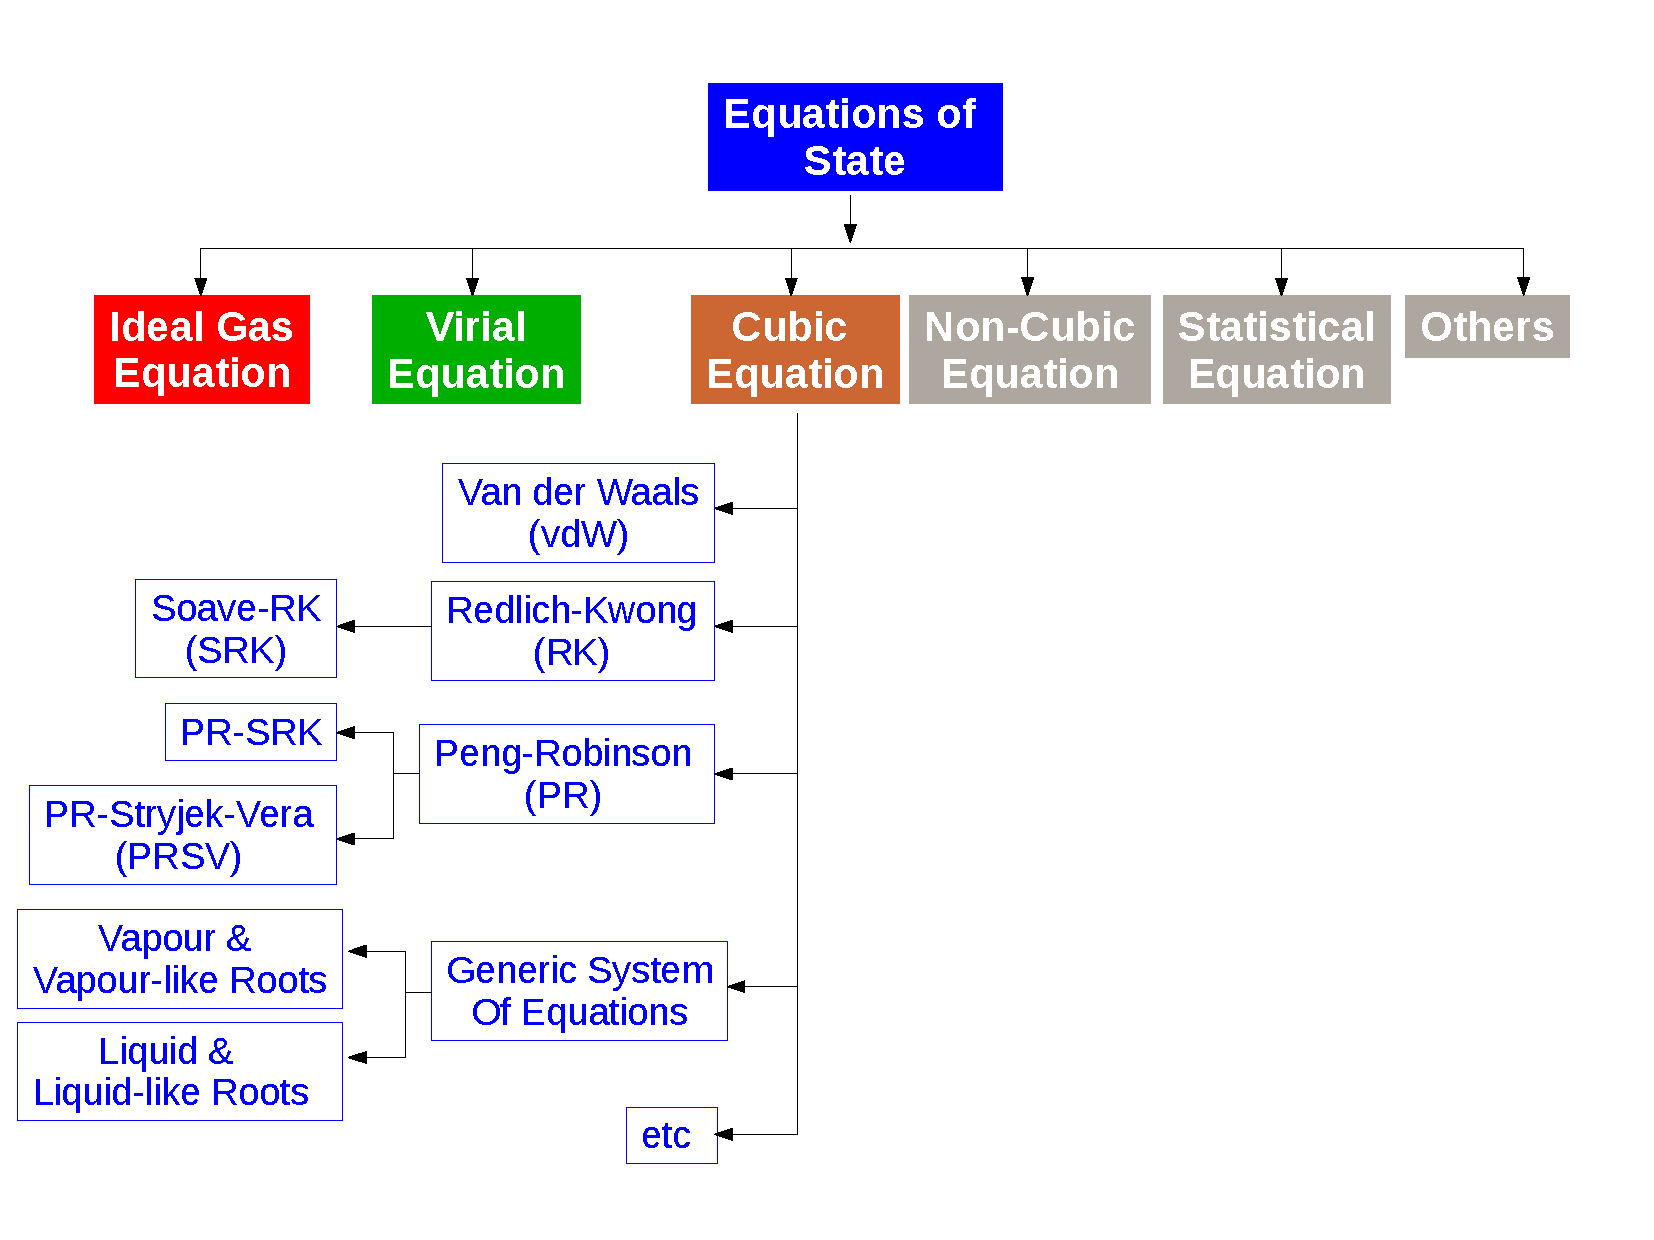
\includegraphics[width=0.9\columnwidth,clip]{./Pics/ListEOS}
        \end{center}
      \end{figure}}
\end{frame}
\normalsize


%%%
%%% SUBSECTION
%%%
\subsection{Virial EOS}

%%%
%%% Slide
%%%
\scriptsize
\begin{frame}
 \frametitle{Virial Expansion}
   \begin{columns}
    \begin{column}[l]{0.5\linewidth}
      \begin{enumerate} \scriptsize
        \item<1-> $\left(PV\right)$ along an isotherm can be expressed as function of {\bf P} by a \textcolor{blue}{power series},
           \visible<1->{\begin{displaymath}
             \left(PV\right) = a + bP + cP^{2} + dP^{3} + \cdots
           \end{displaymath}}
        \item<2-> Defining $b=aB^{\prime}$, $c=aC^{\prime}$, $d=aD^{\prime}$, $\cdots$, then
           \visible<2->{\begin{equation}\label{Mod3:VirialEoS1}
             \left(PV\right) = a\left( 1 + B^{\prime}P + C^{\prime}P^{2} + D^{\prime}P^{3} + \cdots\right) 
           \end{equation}}
        \item<2-> $B^{\prime}$, $C^{\prime}$ and $D^{\prime}$ are constants, characteristic for each chemical species and temperature-dependent $\left(\text{i.e.,} B^{\prime}=B^{\prime}(T), C^{\prime}=C^{\prime}(T)\right)$  
        \item<3-> In the limit case -- $P\rightarrow 0$, \textcolor{blue}{$\left(PV\right)$ for all gases}:\\
           \begin{displaymath}
              \visible<3->{\textcolor{blue}{\left(PV\right)^{\star} =}} 
                   \begin{cases}
                      \visible<3->{a = f\left(T\right)} \\
                      \visible<4->{\textcolor{blue}{a= RT}}\\ 
                   \end{cases}
           \end{displaymath}
           \visible<4->{where $R$ is a proportionally constant, i.e.,  universal gas constant.}
        \item<5-> At this limiting case, $\left(PV\right)_{T}^{\star} = R \times 273.16$. 
      \end{enumerate}
    \end{column}
    \begin{column}[l]{0.5\linewidth}\scriptsize
     \begin{enumerate}\setcounter{enumi}{5}
       \item<6->For \textcolor{blue}{ideal gasses}, pressure is sufficiently small $\left(P\rightarrow 0\right)$. 
       \item<6-> This means that the molecules are separated by infinite distances, and therefore the \textcolor{blue}{intermolecular forces approaches zero}. 
     \end{enumerate}
      \visible<3->{\begin{figure}%
        \begin{center}
          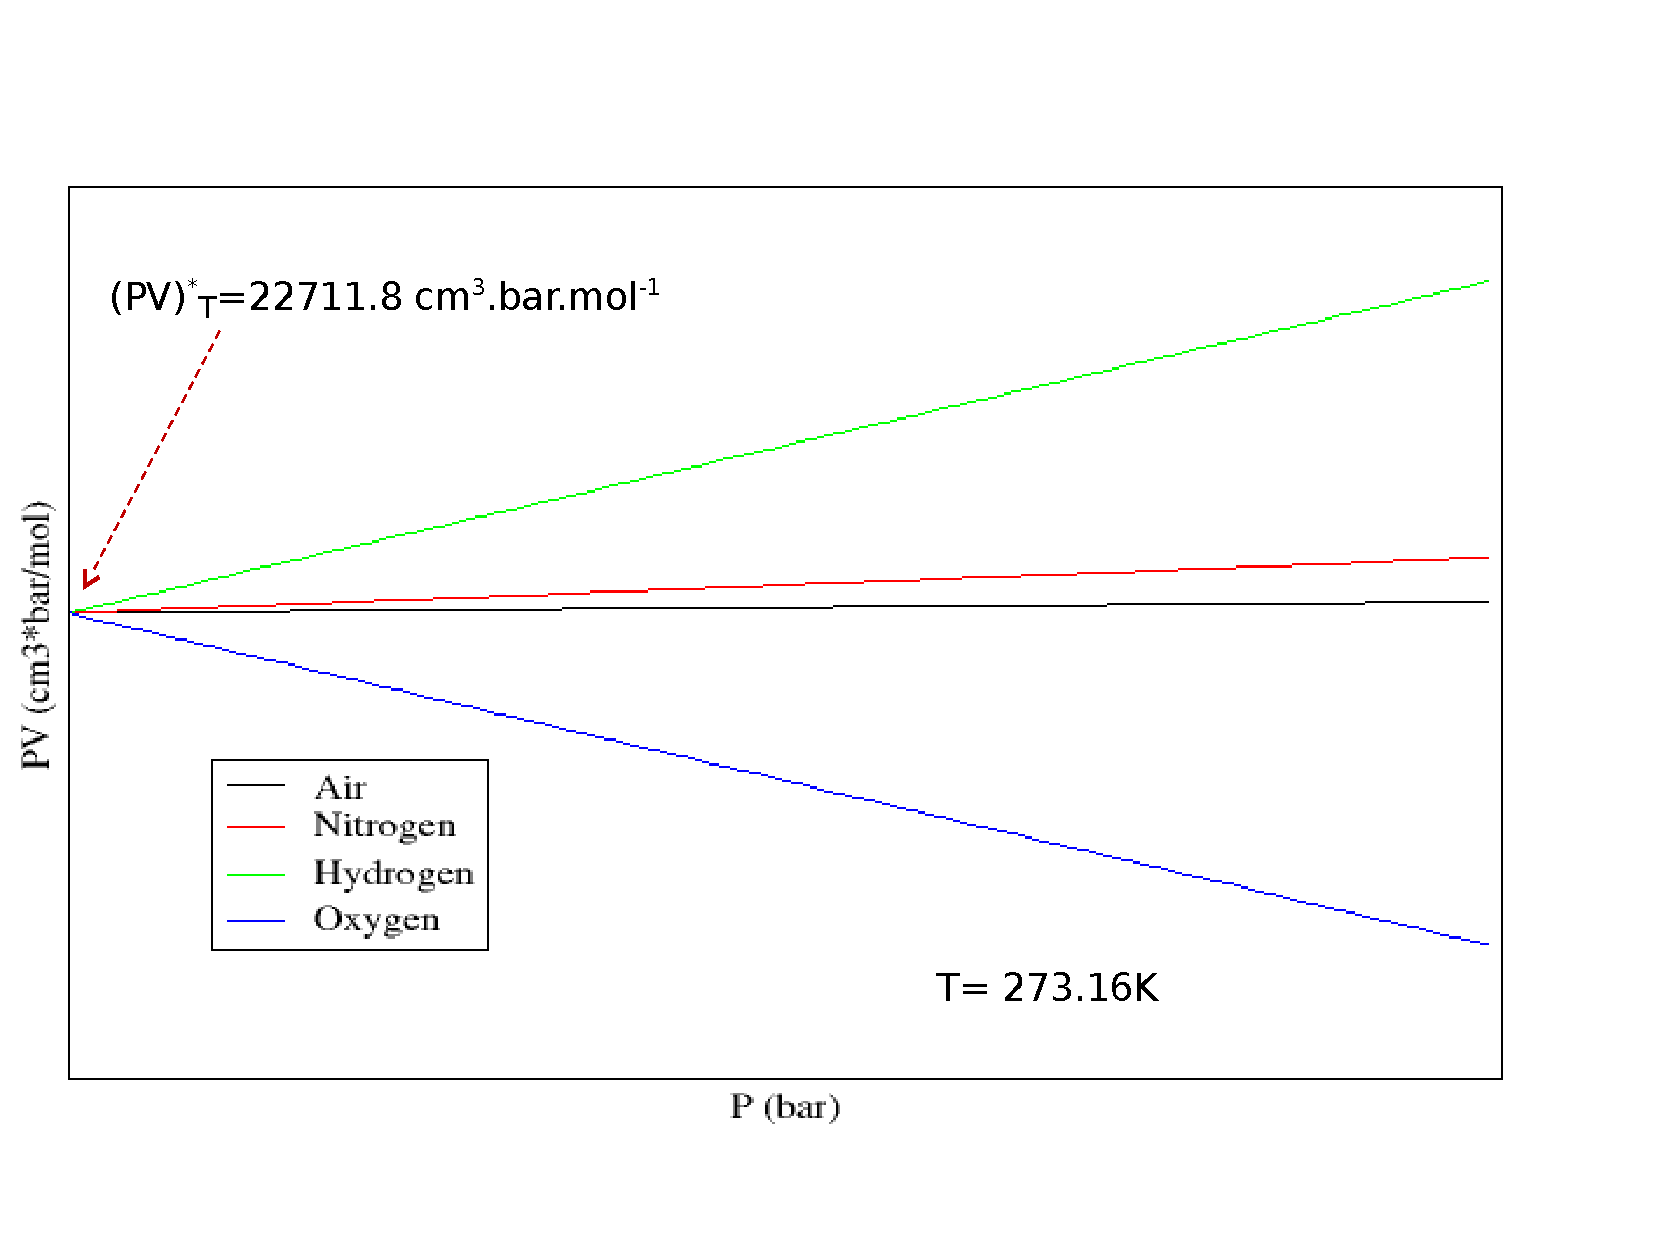
\includegraphics[width=1.05\columnwidth,clip]{./Pics/Virial_EOS}
        \end{center}
      \end{figure}}
    \end{column}
  \end{columns}

\end{frame}
\normalsize


%%%
%%% Slide
%%%
\scriptsize
\begin{frame}
 \frametitle{Compressibility Factor -- $Z$}
   \begin{enumerate}\setcounter{enumi}{7}\scriptsize
     \item<1-> The {\it Virial expansion} is considered the only EOS based on rigorous mathematical derivation. It can also be derived from statistical mechanics leading to physical  significance of the virial coefficients;
     \item<2->The original form of the Virial EOS (Eqn.~\ref{Mod3:VirialEoS1}) can be rewritten as
        \begin{equation}\label{Mod3:VirialEoS2}
            \visible<2->{\frc{PV}{RT}} \visible<3->{ = \textcolor{red}{Z}} = \visible<2->{1 + B^{\prime}P + C^{\prime}P^{2} + D^{\prime}P^{3} + \cdots}
        \end{equation}
     \item<4-> \textcolor{red}{$Z$} is the \textcolor{blue}{compressibility factor} and is commonly used to estimate the deviation from ideal gas behaviour.
     \item<5->Therefore, the Virial EOS can be represented by 2 main forms:
        \begin{equation}
          Z = \frc{PV}{RT} =
             \begin{cases}
                1 + \textcolor{blue}{\frc{B}{V}} + \textcolor{red}{\frc{C}{V^{2}}} + \textcolor{purple}{\frc{D}{V^{3}}} + \cdots \\
                \visible<6->{1 + \blue{B^{\prime}P} + \red{C^{\prime}P^{2}} + \purple{D^{\prime}P^{3}} + \cdots} \\
                \visible<7->{1 + \blue{\frc{B}{RT}P} + \red{\frc{C-B^{2}}{\left(RT\right)^{2}}P^{2}} + \purple{\frc{D-3BC+2B^{2}}{\left(RT\right)^{3}}P^{3}} + \cdots}
             \end{cases}
        \end{equation}
     \item<8-> Thus, for real cases
        \begin{equation}
          \visible<8->{Z = \frc{PV}{RT} =}
             \begin{cases}
                \visible<8->{1 + \blue{B^{\prime}P} = 1 + \blue{\frc{BP}{RT}} \hspace{2.6cm} \Rightarrow\;\; \text{Low-Moderate pressures -- P}<\text{15 bar}}\\
                \visible<9->{1 + \blue{B^{\prime}P} + \red{C^{\prime}P^{2}}  = 1 + \blue{\frc{BP}{RT}} + \red{\frc{C-B^{2}}{\left(RT\right)^{2}}P^{2}}\;\;\Rightarrow\;\; \text{High pressures \red{but} below the } P_{c}}
             \end{cases}
        \end{equation}
             
   \end{enumerate}
\end{frame}
\normalsize


%%%
%%% SUBSECTION
%%%
\subsection{Cubic EOS}

%%%
%%% Slide
%%%
\scriptsize
\begin{frame}
 \frametitle{Generic Cubic EOS}
    \begin{enumerate}\scriptsize
      \item<1-> The simplest equations able to represent both \blue{liquid} and \blue{vapour} phases behaviour but \red{not} for two-phase condition;
      \item<2-> They are designed to be used in a wide range of temperature and pressure;
      \item<3-> General format of a cubic equation on $V$,
         \begin{equation}\label{Mod3:GenCubicEqn}
            \visible<3->{
             P = \frc{RT}{V-b} - \frc{\theta\left(V-\eta\right)}{\left(V-b\right)\left(V^{2}+\kappa V + \lambda\right)}
            }
         \end{equation}
         \visible<3->{Where $b$, $\theta$, $\kappa$, $\lambda$ and $\eta$ are parameters that depend on \blue{T} and \blue{composition} (for mixtures).}
      \item<4-> If $\eta=b$, $\theta=a(T)$,$\kappa=\left(\epsilon+\sigma\right)b$ and $\lambda=\epsilon\sigma b^{2}$, we can define a generic cubic equation of state,
           \visible<4->{\begin{equation}\label{Mod3:GenCubicEOS}
              P = \frc{RT}{V-b} - \frc{a(T)}{\left(V-\epsilon b\right)\left(V+\sigma b\right)}
           \end{equation}
           where $\epsilon$ and $\sigma$ are constants.}
       \item<5-> $a(T)$ and $b$ are specific for chemical species and defined as,
           \visible<5->{\begin{displaymath} 
             a(T) = \Psi\frc{\alpha(T)R^{2}T_{c}^{2}}{P_{c}}\;\;\;\text{ and }\;\;\; b=\Omega\frc{R T_{c}}{P_{c}}
           \end{displaymath}
           $\Psi$ and $\Omega$ are constants and may vary for different cubic EOS.} 
    \end{enumerate}
\end{frame}
\normalsize

%%%
%%% Slide
%%%
\scriptsize
\begin{frame}
 \frametitle{Cubic Equations of State}
    \visible<1->{\begin{block}{van der Waals}
        If we set $\eta=b$, $\theta=a$ and $\kappa=\lambda=0$, Eqn.~\ref{Mod3:GenCubicEqn} reduces to 
        \begin{equation}\label{Mod3:vdWEOS}
              P = \frc{RT}{V-b} - \frc{a(T)}{V^{2}}
        \end{equation}
        with $a=\frc{27 R^{2}T_{c}^{2}}{64 P_{c}}$ and $b=\frc{R T_{c}}{8 P_{c}}$.
    \end{block}}    

    \visible<2->{\begin{block}{Redlich-Kwong}
        \begin{equation}\label{Mod3:vdWEOS}
              P = \frc{RT}{V-b} - \frc{a}{\sqrt{T_{r}}\left(V + b\right)V}
        \end{equation}
       with $a = 0.42748\frc{R^{2}T_{c}^{2}}{P_{c}}$ and $b=0.08664\frc{R T_{c}}{P_{c}}$.
    \end{block}}    

\end{frame}
\normalsize

%%%
%%% Slide
%%%
\scriptsize
\begin{frame}
 \frametitle{Cubic Equations of State}
    \visible<1->{\begin{block}{Soave-Redlich-Kwong}
        \begin{equation}\label{Mod3:SRKEOS}
              P = \frc{RT}{V-b} - \frc{a\alpha}{V\left(V+b\right)}
        \end{equation}
        with $\alpha = \left[1+\gamma\left(1-\sqrt{T_{r}}\right)\right]^{2}$ and $\gamma=0.480+1.574\omega-0.176\omega^{2}$, where $T_{r}=\frc{T}{T_{c}}$.
    \end{block}}    

    \visible<2->{\begin{block}{Peng-Robinson}
        \begin{equation}\label{Mod3:PREOS} 
              P = \frc{RT}{V-b} - \frc{a\alpha}{V\left(V+b\right)+b\left(V-b\right)}
        \end{equation}
       with  $\gamma=0.37464+1.54226\omega-0.26992\omega^{2}$, $a=0.45724\frc{R^{2}T_{c}^{2}}{P_{c}}$ and $b=0.07780\frc{R T_{c}}{P_{c}}$
    \end{block}}    

\end{frame}
\normalsize


%%%
%%% Slide
%%%
%\scriptsize
\begin{frame}
 \frametitle{Cubic Equations of State}
   \visible<1->{\begin{block}{Theorem of Corresponding States (TCS)}
     \blue{$\lq$All fluids, when compared at the same reduced temperature $\left(T_{r}\right)$ and pressure $\left(P_{r}\right)$, have approximately the same compressibility factor $(Z)$, and all deviate from ideal behaviour to about the same degree.'}
     \begin{displaymath}
           T_{r}\equiv\frc{T}{T_{c}} \hspace{3cm} P_{r} \equiv \frc{P}{P_{c}}
     \end{displaymath}
   \end{block}}
   \begin{enumerate}
     \item<2-> TCS is exact for \blue{simple fluids}, e.g., $Ar$, $Kr$ and $Xe$.
     \item<3-> However, larger deviations are observed for \blue{more complex fluids}. 
     \item<4-> Thus, an \red{acentric factor $\left(\omega\right)$} was introduced,
         \begin{displaymath}
            \omega \equiv 1 -\log\left(P^{\text{sat}}_{r}\right)_{T_{r}=0.7}
         \end{displaymath}
         where $\left(P_{r}^{\text{sat}}\right)_{T_{r}=0.7}$ is the reduced vapour pressure at reduced temperature of 0.7. At $T_{r}=0.7$, $\omega=0$ for $Ar$, $Kr$ and $Xe$.
     \item<5-> $\omega$ can be determined for any fluid based on $T_{c}$, P$_{c}$ and a vapour-pressure measurement at $T_{r}=0.7$. 
   \end{enumerate}

\end{frame}
\normalsize


%%%
%%% Slide
%%%
%\scriptsize
\begin{frame}
 \frametitle{Cubic Equations of State}
    \visible<1->{\begin{block}{Vapour $\&$ Vapour-like Roots}
      \begin{displaymath}
        Z= 1 + \beta - q\beta \frc{Z - \beta} {\left(Z+\varepsilon\beta\right)\left(Z+\sigma\beta\right)}
      \end{displaymath}
      with $\beta=\Omega\frc{P_{r}}{T_{r}}$ and $q=\frc{\Psi\alpha\left(T_{r}\right)}{\Omega T_{r}}$
    \end{block}}


    \visible<2->{\begin{block}{Liquid $\&$ Liquid-like Roots}
      \begin{displaymath}
        Z= 1 + \beta + \left(Z + \epsilon\beta\right)\left(Z+\sigma\beta\right)\left(\frc{1+\beta-Z}{q\beta}\right)
      \end{displaymath}
    \end{block}}

    \visible<3->{Iterative method to solve the expressions above, using $Z=1$ as the initial guess.}


\end{frame}
\normalsize



%%%
%%% Slide
%%%
%\scriptsize
\begin{frame}
 \frametitle{Cubic Equations of State -- Parameters}
    \begin{center}
       \begin{tabular}{| l | c c c c c| }
       \hline
          {\bf EOS}  & {\bf $\alpha$} & {\bf $\sigma$}  & {\bf $\varepsilon$} & {\bf $\Omega$} & {\bf $\Psi$ } \\
       \hline
            vdW      & 1              & 0               & 0                  & 1/8            & 27/64          \\
            RK       & T$_{r}^{-1/2}$  & 1                & 0                  & 0.08664       & 0.42748        \\
           SRK       &$\alpha_{\text{SRK}}$& 1            & 0                   & 0.08664       & 0.42748        \\
            PR       &$\alpha_{\text{PR}}$& 1+$\sqrt{2}$   & 1-$\sqrt{2}$        & 0.07780        & 0.45724  \\
       \hline
       \end{tabular}
    \end{center}
\begin{eqnarray}
\alpha_{\text{SRK}} &=& \left[ 1 + \left( 0.480 + 1.574 \omega - 0.176\omega^{2}\right)\left(1-\sqrt{T_{r}}\right)\right]^{2} \nonumber \\
\alpha_{\text{PR}} &=& \left[ 1 + \left( 0.37464 + 1.54226 \omega - 0.26992\omega^{2}\right)\left(1-\sqrt{T_{r}}\right)\right]^{2} \nonumber
\end{eqnarray}

\end{frame}
\normalsize

\section{Summary}

%%%
%%% Slide
%%%
%\scriptsize
\begin{frame}
 \frametitle{Summary}
   \begin{enumerate}
     \item Review of phase diagram and Gibbs rule, including
       \begin{enumerate}
         \item $PT$ and $PV$ diagrams and phase equilibrium;
         \item Critical and Triple points;
       \end{enumerate}
     \item Equations of state
       \begin{enumerate}
         \item General formulation;
         \item Parameters for cubic EOS;
         \item 2- and 3- parameters cubic EOS.
       \end{enumerate}
   \end{enumerate}
\end{frame}


\end{document}

%% Aberdeen style guide should be followed when using this
% layout. Their template powerpoint slide is used to extract the
% Aberdeen color and logo but is otherwise ignored (it has little or
% no formatting in it anyway).
%
% http://www.abdn.ac.uk/documents/style-guide.pdf

%%%%%%%%%%%%%%%%%%%% Document Class Settings %%%%%%%%%%%%%%%%%%%%%%%%%
% Pick if you want slides, or draft slides (no animations)
%%%%%%%%%%%%%%%%%%%%%%%%%%%%%%%%%%%%%%%%%%%%%%%%%%%%%%%%%%%%%%%%%%%%%%
%Normal document mode%
\documentclass[10pt,compress]{beamer}
%Draft or handout mode
%\documentclass[10pt,compress,handout]{beamer}
%\documentclass[10pt,compress,handout,ignorenonframetext]{beamer}

%%%%%%%%%%%%%%%%%%%% General Document settings %%%%%%%%%%%%%%%%%%%%%%%
% These settings must be set for each presentation
%%%%%%%%%%%%%%%%%%%%%%%%%%%%%%%%%%%%%%%%%%%%%%%%%%%%%%%%%%%%%%%%%%%%%%
\newcommand{\shortname}{jefferson.gomes@abdn.ac.uk}
\newcommand{\fullname}{Dr Jeff Gomes}
\institute{School of Engineering}
\newcommand{\emailaddress}{}%jefferson.gomes@abdn.ac.uk}
\newcommand{\logoimage}{../../FigBanner/UoAHorizBanner}
\title{Chemical Thermodynamics (EG3029)}
\subtitle{Module 4: Thermodynamic Properties of Pure Fluids}
\date[2014-15]{2014-15}

%%%%%%%%%%%%%%%%%%%% Template settings %%%%%%%%%%%%%%%%%%%%%%%%%%%%%%%
% You shouldn't have to change below this line, unless you want to.
%%%%%%%%%%%%%%%%%%%%%%%%%%%%%%%%%%%%%%%%%%%%%%%%%%%%%%%%%%%%%%%%%%%%%%
\usecolortheme{whale}
\useoutertheme{infolines}

% Use the fading effect for items that are covered on the current
% slide.
\beamertemplatetransparentcovered

% We abuse the author command to place all of the slide information on
% the title page.
\author[\shortname]{%
  \fullname\\\ttfamily{\emailaddress}
}


%At the start of every section, put a slide indicating the contents of the current section.
\AtBeginSection[] {
  \begin{frame}
    \frametitle{Section Outline}
    \tableofcontents[currentsection]
  \end{frame}
}

% Allow the inclusion of movies into the Presentation! At present,
% only the Okular program is capable of playing the movies *IN* the
% presentation.
\usepackage{multimedia}
\usepackage{animate}

%% Handsout -- comment out the lines below to create handstout with 4 slides in a page with space for comments
\usepackage{handoutWithNotes}

\mode<handout>
{
\usepackage{pgf,pgfpages}

\pgfpagesdeclarelayout{2 on 1 boxed with notes}
{
\edef\pgfpageoptionheight{\the\paperheight} 
\edef\pgfpageoptionwidth{\the\paperwidth}
\edef\pgfpageoptionborder{0pt}
}
{
\setkeys{pgfpagesuselayoutoption}{landscape}
\pgfpagesphysicalpageoptions
    {%
        logical pages=4,%
        physical height=\pgfpageoptionheight,%
        physical width=\pgfpageoptionwidth,%
        last logical shipout=2%
    } 
\pgfpageslogicalpageoptions{1}
    {%
    border code=\pgfsetlinewidth{1pt}\pgfstroke,%
    scale=1,
    center=\pgfpoint{.25\pgfphysicalwidth}{.75\pgfphysicalheight}%
    }%
\pgfpageslogicalpageoptions{2}
    {%
    border code=\pgfsetlinewidth{1pt}\pgfstroke,%
    scale=1,
    center=\pgfpoint{.25\pgfphysicalwidth}{.25\pgfphysicalheight}%
    }%
\pgfpageslogicalpageoptions{3}
    {%
    border shrink=\pgfpageoptionborder,%
    resized width=.7\pgfphysicalwidth,%
    resized height=.5\pgfphysicalheight,%
    center=\pgfpoint{.75\pgfphysicalwidth}{.29\pgfphysicalheight},%
    copy from=3
    }%
\pgfpageslogicalpageoptions{4}
    {%
    border shrink=\pgfpageoptionborder,%
    resized width=.7\pgfphysicalwidth,%
    resized height=.5\pgfphysicalheight,%
    center=\pgfpoint{.75\pgfphysicalwidth}{.79\pgfphysicalheight},%
    copy from=4
    }%

\AtBeginDocument
    {
    \newbox\notesbox
    \setbox\notesbox=\vbox
        {
            \hsize=\paperwidth
            \vskip-1in\hskip-1in\vbox
            {
                \vskip1cm
                Notes\vskip1cm
                        \hrule width\paperwidth\vskip1cm
                    \hrule width\paperwidth\vskip1cm
                        \hrule width\paperwidth\vskip1cm
                    \hrule width\paperwidth\vskip1cm
                        \hrule width\paperwidth\vskip1cm
                    \hrule width\paperwidth\vskip1cm
                    \hrule width\paperwidth\vskip1cm
                    \hrule width\paperwidth\vskip1cm
                        \hrule width\paperwidth
            }
        }
        \pgfpagesshipoutlogicalpage{3}\copy\notesbox
        \pgfpagesshipoutlogicalpage{4}\copy\notesbox
    }
}
}

%\pgfpagesuselayout{2 on 1 boxed with notes}[letterpaper,border shrink=5mm]

%%%%% Color settings
\usepackage{color}
%% The background color for code listings (i.e. example programs)
\definecolor{lbcolor}{rgb}{0.9,0.9,0.9}%
\definecolor{UoARed}{rgb}{0.64706, 0.0, 0.12941}
\definecolor{UoALight}{rgb}{0.85, 0.85, 0.85}
\definecolor{UoALighter}{rgb}{0.92, 0.92, 0.92}
\setbeamercolor{structure}{fg=UoARed} % General background and higlight color
\setbeamercolor{frametitle}{bg=black} % General color
\setbeamercolor{frametitle right}{bg=black} % General color
\setbeamercolor{block body}{bg=UoALighter} % For blocks
\setbeamercolor{structure}{bg=UoALight} % For blocks
% Rounded boxes for blocks
\setbeamertemplate{blocks}[rounded]

%%%%% Font settings
% Aberdeen requires the use of Arial in slides. We can use the
% Helvetica font as its widely available like so
% \usepackage{helvet}
% \renewcommand{\familydefault}{\sfdefault}
% But beamer already uses a sans font, so we will stick with that.

% The size of the font used for the code listings.
\newcommand{\goodsize}{\fontsize{6}{7}\selectfont}

% Extra math packages, symbols and colors. If you're using Latex you
% must be using it for formatting the math!
\usepackage{amscd,amssymb} \usepackage{amsfonts}
\usepackage[mathscr]{eucal} \usepackage{mathrsfs}
\usepackage{latexsym} \usepackage{amsmath} \usepackage{bm}
\usepackage{amsthm} \usepackage{textcomp} \usepackage{eurosym}
% This package provides \cancel{a} and \cancelto{a}{b} to "cancel"
% expressions in math.
\usepackage{cancel}

\usepackage{comment} 

% Get rid of font warnings as modern LaTaX installations have scalable
% fonts
\usepackage{type1cm} 

%\usepackage{enumitem} % continuous numbering throughout enumerate commands

% For exact placement of images/text on the cover page
\usepackage[absolute]{textpos}
\setlength{\TPHorizModule}{1mm}%sets the textpos unit
\setlength{\TPVertModule}{\TPHorizModule} 

% Source code formatting package
\usepackage{listings}%
\lstset{ backgroundcolor=\color{lbcolor}, tabsize=4,
  numberstyle=\tiny, rulecolor=, language=C++, basicstyle=\goodsize,
  upquote=true, aboveskip={1.5\baselineskip}, columns=fixed,
  showstringspaces=false, extendedchars=true, breaklines=false,
  prebreak = \raisebox{0ex}[0ex][0ex]{\ensuremath{\hookleftarrow}},
  frame=single, showtabs=false, showspaces=false,
  showstringspaces=false, identifierstyle=\ttfamily,
  keywordstyle=\color[rgb]{0,0,1},
  commentstyle=\color[rgb]{0.133,0.545,0.133},
  stringstyle=\color[rgb]{0.627,0.126,0.941}}

% Allows the inclusion of other PDF's into the final PDF. Great for
% attaching tutorial sheets etc.
\usepackage{pdfpages}
\setbeamercolor{background canvas}{bg=}  

% Remove foot note horizontal rules, they occupy too much space on the slide
\renewcommand{\footnoterule}{}

% Force the driver to fix the colors on PDF's which include mixed
% colorspaces and transparency.
\pdfpageattr {/Group << /S /Transparency /I true /CS /DeviceRGB>>}

% Include a graphics, reserve space for it but
% show it on the next frame.
% Parameters:
% #1 Which slide you want it on
% #2 Previous slides
% #3 Options to \includegraphics (optional)
% #4 Name of graphic
\newcommand{\reserveandshow}[4]{%
\phantom{\includegraphics<#2|handout:0>[#3]{#4}}%
\includegraphics<#1>[#3]{#4}%
}

\newcommand{\frc}{\displaystyle\frac}
\newcommand{\red}{\textcolor{red}}
\newcommand{\blue}{\textcolor{blue}}
\newcommand{\green}{\textcolor{green}}
\newcommand{\purple}{\textcolor{purple}}
 
\begin{document}

% Title page layout
\begin{frame}
  \titlepage
  \vfill%
  \begin{center}
    \includegraphics[clip,width=0.8\textwidth]{\logoimage}
  \end{center}
\end{frame}

% Table of contents
\frame{ \frametitle{Slides Outline}
  \tableofcontents
}


%%%%%%%%%%%%%%%%%%%% The Presentation Proper %%%%%%%%%%%%%%%%%%%%%%%%%
% Fill below this line with \begin{frame} commands! It's best to
% always add the fragile option incase you're going to use the
% verbatim environment.
%%%%%%%%%%%%%%%%%%%%%%%%%%%%%%%%%%%%%%%%%%%%%%%%%%%%%%%%%%%%%%%%%%%%%%


%%%
%%% SECTION
%%%
%\section{General Remarks}

%%%
%%% Slides
%%%
\begin{frame}
 \frametitle{Aims and Objectives}
   \begin{enumerate}
     \item<1-> In Modules 1-3, we learnt:
       \begin{enumerate}
         \item<1-> the laws of Thermodynamics and how they describe thermal equilibrium of species in closed and opened systems;
         \item<1-> how to calculate thermodynamics properties -- internal energy, enthalpy and entropy for pure chemicallspecies;
         \item<1-> PVT behaviour of pure species in equilibrium and;
         \item<1-> Equations of state.
       \end{enumerate} 
     \item<2-> This Module focuses on 
         \begin{enumerate}
           \item<2-> Thermodynamic properties of pure fluids;
           \item<2-> Introduce two remaining thermodynamic properties: Gibbs and Helmholtz free energies;
           \item<2-> Maxwell relations.
         \end{enumerate}
   \end{enumerate}

\end{frame}


%%%
%%% SECTION
%%%
%\section{Bibliography}
\begin{frame}
 \frametitle{Suggested References}
  Literature relevant for this module:
  \begin{enumerate}[(a)]
   \item\label{SVN_Book} J.M. Smith, H.C. Van Ness, M.M. Abbott, $\lq$Introduction to Chemical Engineering Thermodynamics', 6$^{th}$ Edition: Chapter 6;
   \item Y.A. Cengel, M.A. Boles, $\lq$Thermodynamics -- An Engineering Approach', 5$^{th}$ Edition: Chapter 12.1-4; 
   %\item M.J. Moran, H.N. Saphiro, D.D. Boettner, M.B. Bailey, $\lq$Principles of Engineering Thermodynamics', 7$^{th}$ Edition: Chapters 3;
   %\item C. Borgnakke, R.E. Sonntag,$\lq$Fundamentals of Thermodynamics',8$^{th}$ Edition: Chapter 2.
   \item S.I. Sandler, $\lq$Chemical, Biochemical and Engineering Thermodynamics', 4$^{th}$ Edition: Chapter 6.
  \end{enumerate}
\end{frame}


%%%
%%% SECTION
%%%
\section{Property Relations for Homogeneous Phases}

%%%
%%% SUBSECTION
%%%
\subsection{Thermodynamic Potentials} 


%%%
%%% Slide
%%%
%\scriptsize
\begin{frame}
  \frametitle{New State Functions}
   \visible<1->{\begin{block}{Enthalpy}
      \begin{displaymath}
         H = U + P V
      \end{displaymath}
   \end{block}
   }
   \visible<2->{\begin{block}{Gibbs Free Energy}
      \begin{displaymath}
         G = H - T S
      \end{displaymath}
   \end{block}
   }
   \visible<3->{\begin{block}{Helmholtz Free Energy}
      \begin{displaymath}
         A = U - T S
      \end{displaymath}
   \end{block}
   }

\end{frame}
\normalsize

%%%
%%% SUBSECTION
%%%
\subsection{Maxwell's Relations}
%%%
%%% Slide
%%%
%\scriptsize
\begin{frame}
  \frametitle{Maxwell's Relations}
   \visible<1->{\begin{block}{For 1 mol of homogeneous fluid at $T=$ constant}
      \begin{center}
        \begin{tabular}{l c  l}
           $sU = T dS - PdV$  &  \hspace{1cm} & $dH = TdS + VdP$ \\
           $dA = -PdV - SdT$  &  \hspace{1cm} & $dG = VdP - SdT$ 
        \end{tabular}
      \end{center}
   \end{block}
   }
   \visible<2->{\begin{block}{Maxwell's Equations}
      \begin{center}
        \begin{tabular}{l c  l}
           $\left(\frc{\partial T}{\partial V}\right)_{S} = -\left(\frc{\partial P}{\partial S}\right)_{v}$  &  \hspace{1cm} & $\left(\frc{\partial T}{\partial P}\right)_{S} =  \left(\frc{\partial V}{\partial S}\right)_{P}$  \\
           $\left(\frc{\partial P}{\partial T}\right)_{V} =  \left(\frc{\partial S}{\partial V}\right)_{T}$  &  \hspace{1cm} & $\left(\frc{\partial V}{\partial T}\right)_{S} = -\left(\frc{\partial S}{\partial P}\right)_{T}$ 
        \end{tabular}
      \end{center}
   \end{block}
   }

\end{frame}
\normalsize


%%%
%%% SUBSECTION
%%%
\subsection{Thermodynamic Potentials: Dependence on $T$ and $P$}

%%%
%%% Slide
%%%
%\scriptsize
\begin{frame}
  \frametitle{Internal Energy, Enthalpy and Entropy}
   \visible<1->{\begin{block}{$H$ and $S$ as functions of $T$ and $P$}
      \begin{center}
        \begin{tabular}{l c  l}
           $dH = C_{p}dT + \left[ V - T\left(\frc{\partial V}{\partial T}\right)_{P}\right]dP$ &  \hspace{1cm} & $dS=C_{p}\frc{dT}{T} - \left(\frc{\partial V}{\partial T}\right)_{P}dP$
        \end{tabular}
      \end{center}
   \end{block}
   }
   \visible<2->{\begin{block}{Ideal Gas}
      \begin{center}
        \begin{tabular}{l c  l}
           $dH = C_{p}dT$  &  \hspace{1cm} & $dS=C_{p}\frc{dT}{T} - R\frc{dP}{P}$  
        \end{tabular}
      \end{center}
   \end{block}
   }
   \visible<3->{\begin{block}{Liquid}
      \begin{center}
        \begin{tabular}{l c  l}
           $dH = C_{p}dT + \left(1-\beta\right)VdP$  &  \hspace{1cm} & $dS = C_{p}\frc{dT}{T} - \beta V{dP}$  
        \end{tabular}
      \end{center}
   \end{block}
   }
   \visible<4->{\begin{block}{$U$ and $S$ as functions of $T$ and $V$}
      \begin{center}
        \begin{tabular}{l c  l}
           $dU = C_{v}dT + \left[T\left(\frc{\partial P}{\partial T}\right)_{V} - P\right]dV$  &  \hspace{1cm} & $dS = C_{v}\frc{dT}{T} - \left(\frc{\partial P}{\partial T}\right)_{V}dV$  
        \end{tabular}
      \end{center}
   \end{block}
   }

\end{frame}
\normalsize


%%%
%%% Slide
%%%
%\scriptsize
\begin{frame}
  \frametitle{Gibbs Free Energy as Differential Operator}
     \begin{enumerate}[(a)]
        \item<1-> Gibbs Energy as generating function:
              \begin{displaymath}
                 \visible<1->{dG = VdP - SdT} \visible<2->{\Longrightarrow d\left(\frc{G}{RT}\right) = \frc{1}{RT}dG - \frc{G}{RT^{2}}dT} \nonumber 
              \end{displaymath}

        \item<3-> After substitution $\&$ algebraic reduction:
              \begin{displaymath}
                  \visible<3->{\frc{V}{RT} = \left\{ \frc{\partial\left(\frc{G}{RT}\right)}{\partial P}\right\}_{T} \hspace{1cm}\text{and}\hspace{1cm} \frc{H}{RT} = -T\left\{ \frc{\partial\left(\frc{G}{RT}\right)}{\partial T}\right\}_{P}}
              \end{displaymath}

        \item<4-> \textcolor{blue}{The Gibbs free energy when expressed as $G\left(T,P\right)$ operates as a generating function for other thermodynamic properties, and implicitly represents complete property information.}
     \end{enumerate}

\end{frame}
\normalsize

%%%
%%% SECTION
%%%
\section{Residual Properties}

\subsection{General Approach}
%%%
%%% Slide
%%%
%\scriptsize
\begin{frame}
  \frametitle{Residual Properties: General Approach}
     \begin{enumerate}[(a)]
        \item<1-> \textcolor{blue}{Residual Gibbs energy} is defined as:
              \visible<1->{\begin{displaymath}
                 \textcolor{red}{G^{R} = G - G^{ig}}
              \end{displaymath}}
            where \textcolor{blue}{$G$} is the actual Gibbs energy and \textcolor{blue}{$G^{id}$} is the correspondent thermodynamic function for ideal gas at same $T$ and $P$;
        \item<2-> This leads to,
              \visible<2->{\begin{displaymath}
                 d\left(\frc{G^{R}}{RT}\right) =\frc{V^{R}}{RT}dP - \frc{H^{R}}{RT^{2}}dT
              \end{displaymath}}
             
              \visible<3->{with,\begin{displaymath}
                 \frc{V^{R}}{RT} = \left\{ \frc{\partial\left(\frc{G^{R}}{RT}\right)}{\partial P}\right\}_{T} \hspace{0.5cm}\text{ and }\hspace{0.5cm} \frc{H^{R}}{RT} = -T\left\{ \frc{\partial\left(\frc{G^{R}}{RT}\right)}{\partial T}\right\}_{P}
              \end{displaymath}}
     \end{enumerate}

\end{frame}
\normalsize


%%%
%%% SUBSECTION
%%%
\subsection{Equations of State}
%%%
%%% Slide
%%%
%\scriptsize
\begin{frame}
  \frametitle{Residual Properties by EOS}
       Alternative approach to numerical integration: analytical solution by EOS:
            \begin{enumerate}[(a)]
                \item<1-> Virial EOS: \textcolor{blue}{$Z = 1 + \frc{BP}{RT}$}, 
                   \visible<2->{leading to \begin{displaymath}
                      \frc{G^{R}}{RT} = \displaystyle\int\limits_{0}^{\rho}\left(Z - 1\right)\frc{d\rho}{\rho} + Z - 1 - \ln Z \hspace{1cm} \frc{H^{R}}{RT} = -T \displaystyle\int\limits_{0}^{\rho}\left(\frc{\partial Z}{\partial T}\right)_{\rho}\frc{d\rho}{\rho} + Z - 1
                   \end{displaymath}
                   \begin{displaymath}
                      \frc{S^{R}}{RT} = \ln Z - T \displaystyle\int\limits_{0}^{\rho} \left(\frc{\partial Z}{\partial T}\right)_{\rho} \frc{d\rho}{\rho} - \displaystyle\int\limits_{0}^{\rho}\left(Z - 1\right)\frc{d\rho}{\rho} 
                   \end{displaymath}
}
             \end{enumerate}
\end{frame}
\normalsize



%%%
%%% Slide
%%%
%\scriptsize
\begin{frame}
  \frametitle{Residual Properties by EOS}
            \begin{enumerate}[(a)]\setcounter{enumi}{1}
               \item<1-> Cubic EOS: \textcolor{blue}{$P = \frc{RT}{V - b} - \frc{a\left(T\right)}{\left(V + \epsilon b\right)\left(V + \sigma b\right)}$}
                   \visible<2->{leading to\begin{displaymath}
                      \frc{G^{R}}{RT} = Z - 1 - \ln\left(Z - \beta\right) - q\mathcal{I} \hspace{1cm} \frc{H^{R}}{RT} = Z - 1 + \left[\frc{d\ln\alpha\left(T_{r}\right)}{d\ln T_{r}} - 1\right]q\mathcal{I}
                   \end{displaymath}
                   \begin{displaymath}
                       \frc{S^{R}}{R} = \ln\left(Z - \beta \right) + \frc{d\ln\alpha\left(T_{r}\right)}{d\ln T_{r}}q\mathcal{I} 
                   \end{displaymath}
                   with
                   \begin{displaymath}
                      \mathcal{I} \equiv \displaystyle\int\limits_{0}^{P} \frc{d\left(\rho b\right)}{\left(1 + \epsilon\rho b\right)\left(1 + \sigma\rho b\right)}\;\;\;\;\left(T\text{ const.}\right)
                   \end{displaymath}
                   See Section 6.3 of Smith, Van Ness $\&$ Abbott -- \textcolor{blue}{Reference (\ref{SVN_Book})}.
}
             \end{enumerate}

\end{frame}
\normalsize





%%%
%%% SECTION
%%%
\section{Two-Phase Systems}

\subsection{General Remarks}
%%%
%%% Slide
%%%
%\scriptsize
\begin{frame}
  \frametitle{General Remarks}
     \begin{enumerate}[(a)]
         \item<1-> \textcolor{blue}{Phase transition}: many extensive properties change abruptly during phase transition at given $P$ and $T$: specific volume, internal energy, enthalpy and entropy;
         \item<2-> \textcolor{blue}{Exception:} \textcolor{red}{molar Gibbs energy};
         \item<3-> For 2 phases \textcolor{blue}{$\alpha$} and \textcolor{blue}{$\beta$} of pure species at equilibrium,
            \visible<3->{\begin{block}{\textcolor{blue}{Equilibrium $\Rightarrow$ Equality of Gibbs energy}}
                     \begin{displaymath}
                        \textcolor{red}{G^{\alpha} = G^{\beta}} 
                     \end{displaymath}
            \end{block}}
         \item<4-> Clapeyron equation:
            \visible<4->{\begin{displaymath}
              \frc{d P^{sat}}{d T} = \frc{\Delta H^{lv}}{T \Delta V^{lv}}
            \end{displaymath}}
     \end{enumerate}

\end{frame}
\normalsize


%%%
%%% Slide
%%%
%\scriptsize
\begin{frame}
  \frametitle{General Remarks}
     \begin{enumerate}[(a)]\setcounter{enumi}{4}
         \item<1-> Temperature dependence of vapour pressure \blue{$\Rightarrow$} Empirical approaches for practical applications:
         \begin{enumerate}[(i)]
            \item<2-> Simplest case:
                \visible<2->{\begin{displaymath}
                   \ln P^{sat} = A - \frc{B}{T}
                \end{displaymath}}
            \item<3-> Antoine Equation:
                \visible<3->{\begin{displaymath}
                   \ln P^{sat} = A - \frc{B}{T+C}
                \end{displaymath}}
            \item<4-> Wagner Equation \blue{(more accurate)}:
                \visible<4->{\begin{displaymath}
                   \ln P_{r}^{sat} = \frc{A\tau + B\tau^{1.5} + C\tau^{3} + D\tau^{6}}{1-\tau}\;\;\;\text{ with }\;\;\; \tau = 1 - T_{r}
                \end{displaymath}}
         \end{enumerate}
     \end{enumerate}

\end{frame}
\normalsize


%%%
%%% SUBSECTION 
%%%
\subsection{Liquid/Vapour Systems}
%%%
%%% Slide
%%%
%\scriptsize
\begin{frame}
  \frametitle{Liquid/Vapour Systems}
     \begin{enumerate}[(a)]
         \item<1-> Systems with \blue{saturated vapour} and \blue{saturated liquid} in \red{equilibrium};
         \item<2-> \blue{Mass/Energy Balance} for any extensive property:
            \visible<3->{\begin{displaymath} 
                nV = n^{(l)}V^{(l)} + n^{(v)}V^{(v)} \;\;\; \Leftrightarrow \;\;\; V = x^{(l)}V^{(l)} + x^{(v)}V^{(v)}
             \end{displaymath}
             where $x^{(j)}$ is the \blue{molar/mass fraction} of phase \blue{j = l, v} $\rightarrow$  $x^{(l)} + x^{(v)} = 1$. 
            }
         \item<4-> The mass/molar volume fraction of vapour, \blue{$x^{(v)}$}, is also called \blue{vapour quality}. 
     \end{enumerate}

\end{frame}
\normalsize


%%%
%%%
%%% SUBSECTION 
%%%
\subsection{Thermodynamic Diagrams}

%%%
%%% Slide
%%%
%\scriptsize
\begin{frame}
  \frametitle{Pressure $\times$ Enthalpy ({\it PH}) Diagram}
      \begin{figure}%
        \begin{center}
          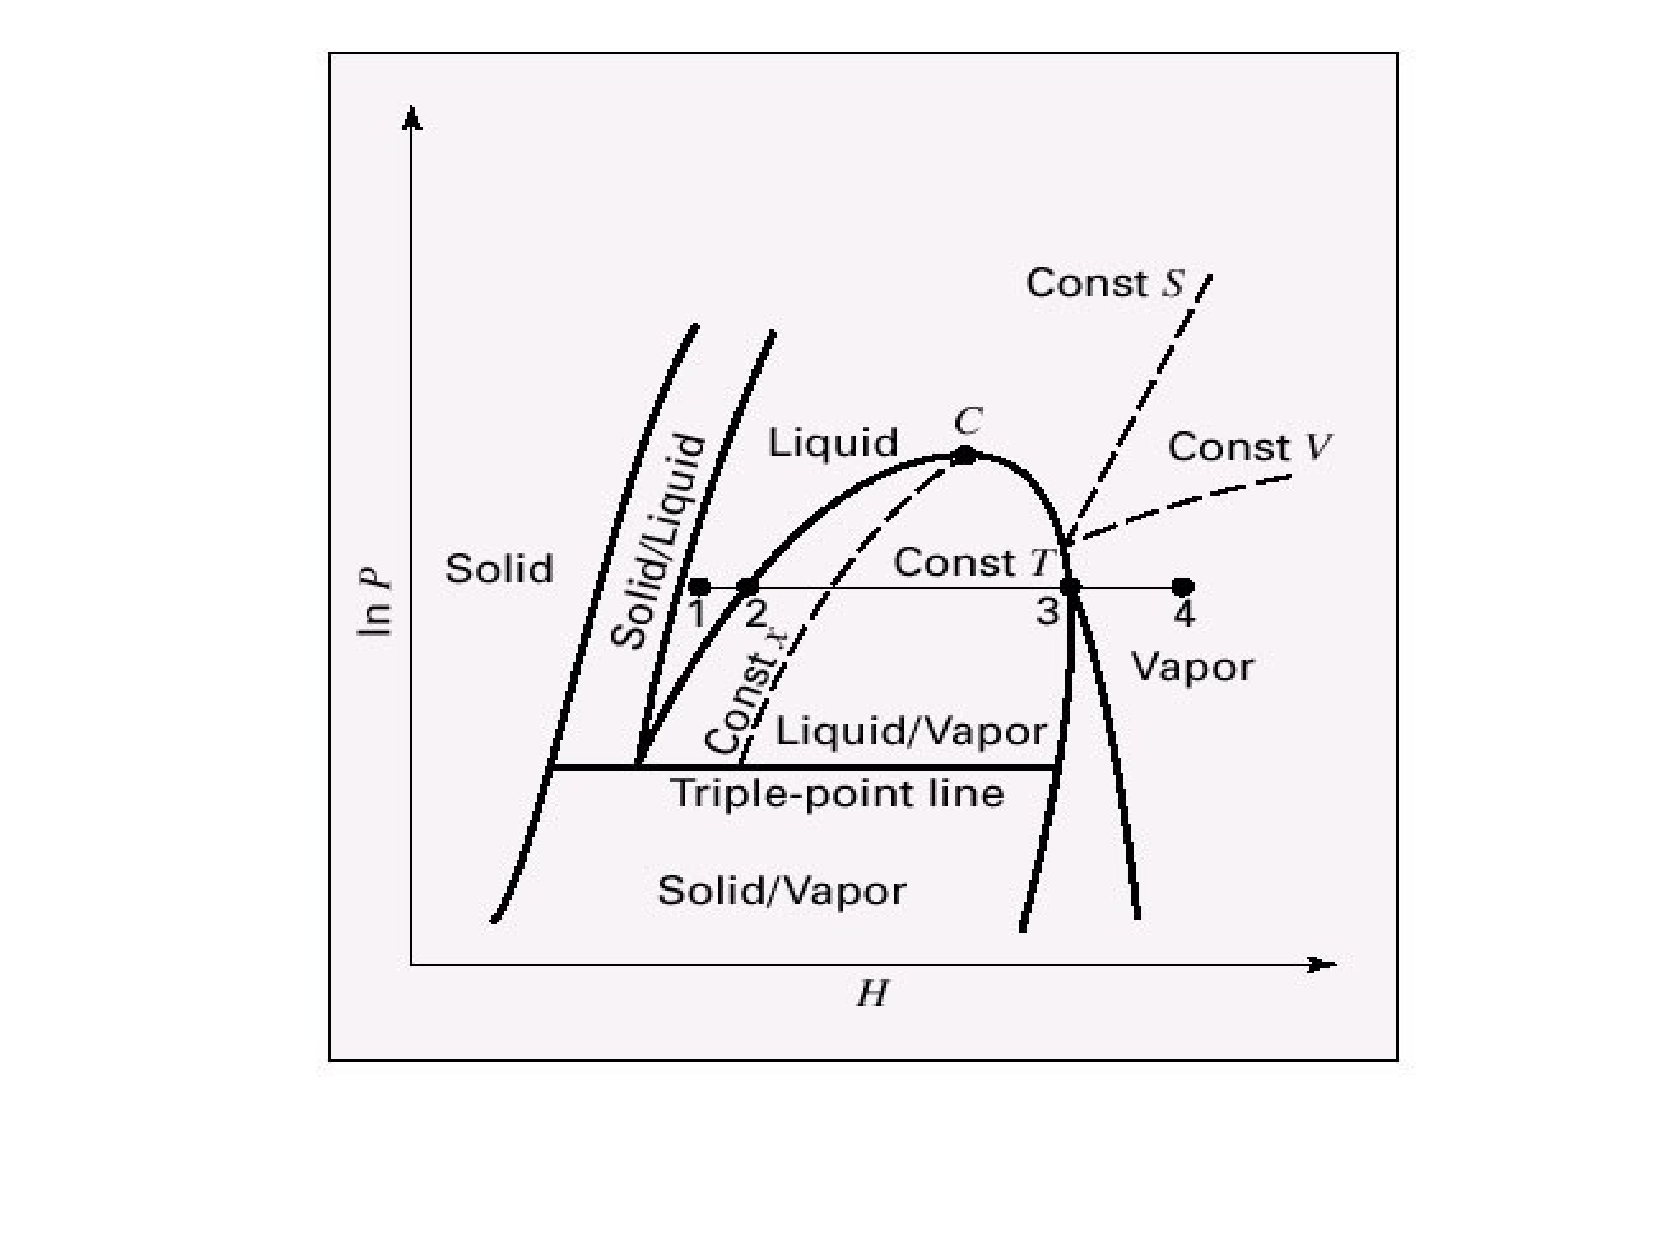
\includegraphics[width=1\columnwidth,clip]{./Pics/LnP_H_Diagram}
        \end{center}
      \end{figure}
\end{frame}
\normalsize


%%%
%%% Slide
%%%
%\scriptsize
\begin{frame}
  \frametitle{Temperature $\times$ Entropy ({\it TS}) Diagram}
      \begin{figure}%
        \begin{center}
          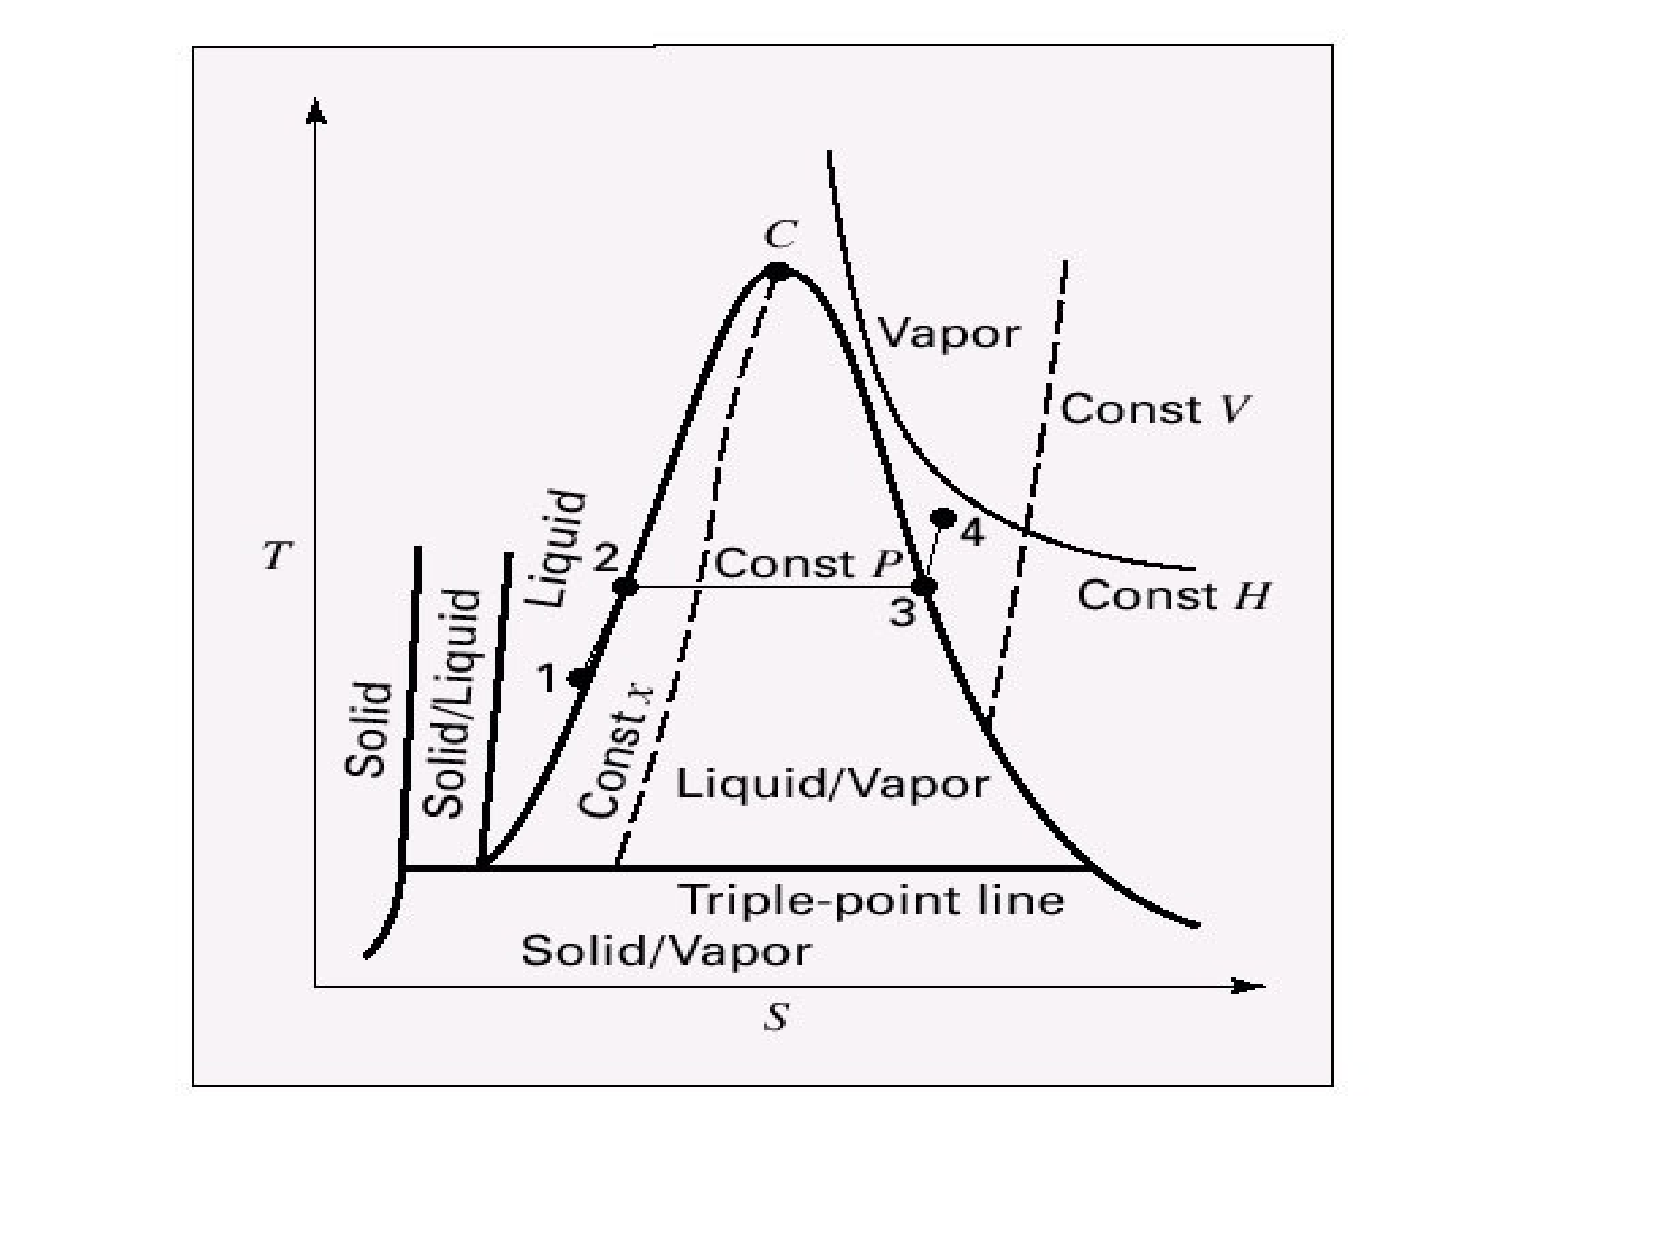
\includegraphics[width=1\columnwidth,clip]{./Pics/T_S_Diagram}
        \end{center}
      \end{figure}
\end{frame}
\normalsize

%%%
%%% Slide
%%%
%\scriptsize
\begin{frame}
  \frametitle{Enthalpy $\times$ Entropy ({\it Moiller}) Diagram}
      \begin{figure}%
        \begin{center} 
          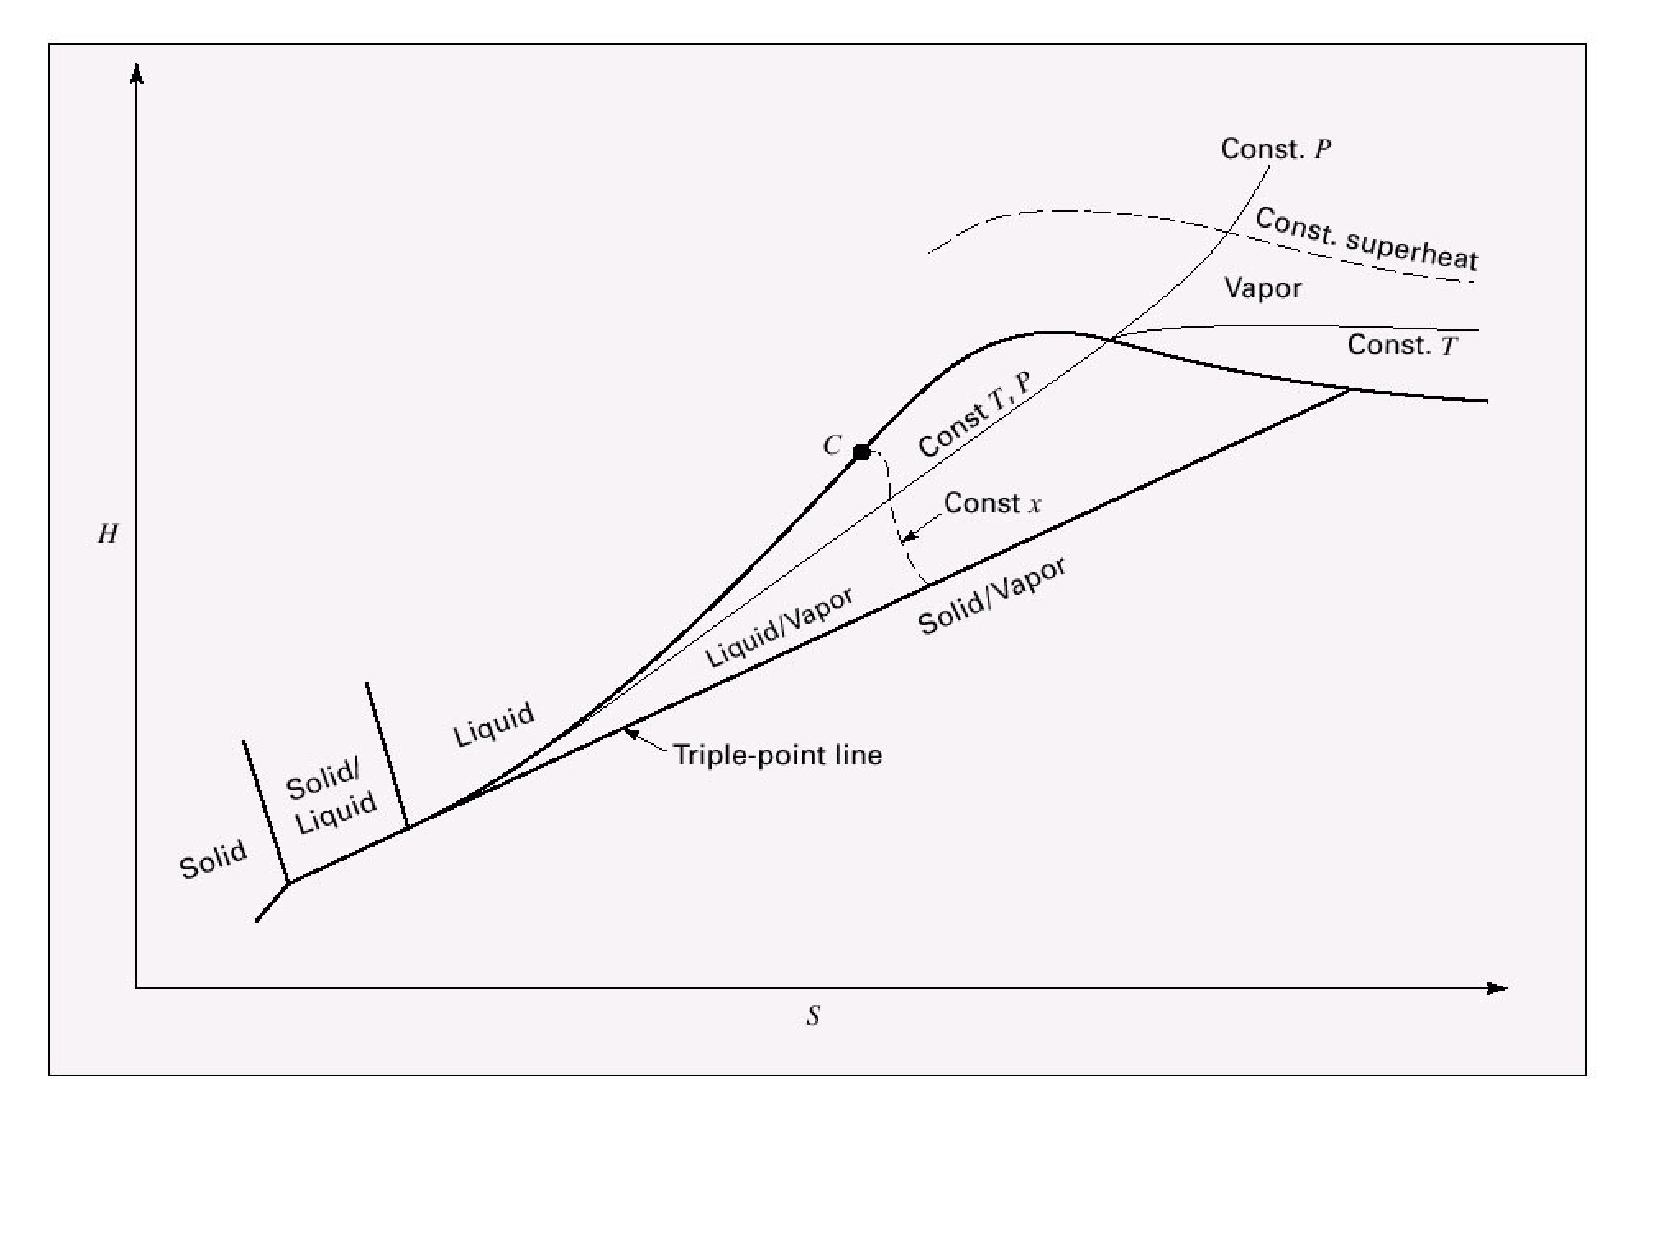
\includegraphics[width=1\columnwidth,clip]{./Pics/MoillerDiagram}
        \end{center}
      \end{figure}
\end{frame}
\normalsize


\section{Summary}

%%%
%%% Slide
%%%
%\scriptsize
\begin{frame}
 \frametitle{Summary}
   \begin{enumerate}[(i)]
     \item New thermodynamic potential properties: Gibbs and Helmholtz free energies;
     \item Introduction of Maxwell's relations and applications;
     \item Internal energy, enthalpy, entropy Gibbs and Helmholtz energies described as functions of pressure, volume and temperature (PVT);
     \item Introduction of residual properties and applications;
     \item Two-phase systems.
   \end{enumerate}
\end{frame}


\end{document}
 

%% Aberdeen style guide should be followed when using this
% layout. Their template powerpoint slide is used to extract the
% Aberdeen color and logo but is otherwise ignored (it has little or
% no formatting in it anyway).
%
% http://www.abdn.ac.uk/documents/style-guide.pdf

%%%%%%%%%%%%%%%%%%%% Document Class Settings %%%%%%%%%%%%%%%%%%%%%%%%%
% Pick if you want slides, or draft slides (no animations)
%%%%%%%%%%%%%%%%%%%%%%%%%%%%%%%%%%%%%%%%%%%%%%%%%%%%%%%%%%%%%%%%%%%%%%
%Normal document mode%
\documentclass[10pt,compress,unknownkeysallowed]{beamer}
%Draft or handout mode
%\documentclass[10pt,compress,handout,unknownkeysallowed]{beamer}
%\documentclass[10pt,compress,handout,ignorenonframetext,unknownkeysallowed]{beamer}

\renewcommand{\insertframenumber}{\theframenumber}
\renewcommand{\theframenumber}{\thesection-\arabic{framenumber}}
\renewcommand{\thesubsectionslide}{\thesection-\arabic{framenumber}} 
\setbeamertemplate{headline}[text line]{This is frame: \insertframenumber}
\AtBeginSection{\setcounter{framenumber}{0}}


%%%%%%%%%%%%%%%%%%%% General Document settings %%%%%%%%%%%%%%%%%%%%%%%
% These settings must be set for each presentation
%%%%%%%%%%%%%%%%%%%%%%%%%%%%%%%%%%%%%%%%%%%%%%%%%%%%%%%%%%%%%%%%%%%%%%
\newcommand{\shortname}{jefferson.gomes@abdn.ac.uk}
\newcommand{\fullname}{Dr Jeff Gomes}
\institute{School of Engineering}
\newcommand{\emailaddress}{}%jefferson.gomes@abdn.ac.uk}
\newcommand{\logoimage}{../../FigBanner/UoAHorizBanner}
\title{Chemical Thermodynamics (EX3029)}
\subtitle{Module 5: Solution Thermodynamics}
\date[ ]{ }

%%%%%%%%%%%%%%%%%%%% Template settings %%%%%%%%%%%%%%%%%%%%%%%%%%%%%%%
% You shouldn't have to change below this line, unless you want to.
%%%%%%%%%%%%%%%%%%%%%%%%%%%%%%%%%%%%%%%%%%%%%%%%%%%%%%%%%%%%%%%%%%%%%%
\usecolortheme{whale}
\useoutertheme{infolines}

% Use the fading effect for items that are covered on the current
% slide.
\beamertemplatetransparentcovered

% We abuse the author command to place all of the slide information on
% the title page.
\author[\shortname]{%
  \fullname\\\ttfamily{\emailaddress}
}


%At the start of every section, put a slide indicating the contents of the current section.
\AtBeginSection[] {
  \begin{frame}
    \frametitle{Section Outline}
    \tableofcontents[currentsection]
  \end{frame}
}

% Allow the inclusion of movies into the Presentation! At present,
% only the Okular program is capable of playing the movies *IN* the
% presentation.
\usepackage{multimedia}
\usepackage{animate}

%% Handsout -- comment out the lines below to create handstout with 4 slides in a page with space for comments
\usepackage{handoutWithNotes}

\mode<handout>
{
\usepackage{pgf,pgfpages}

\pgfpagesdeclarelayout{2 on 1 boxed with notes}
{
\edef\pgfpageoptionheight{\the\paperheight} 
\edef\pgfpageoptionwidth{\the\paperwidth}
\edef\pgfpageoptionborder{0pt}
}
{
\setkeys{pgfpagesuselayoutoption}{landscape}
\pgfpagesphysicalpageoptions
    {%
        logical pages=4,%
        physical height=\pgfpageoptionheight,%
        physical width=\pgfpageoptionwidth,%
        last logical shipout=2%
    } 
\pgfpageslogicalpageoptions{1}
    {%
    border code=\pgfsetlinewidth{1pt}\pgfstroke,%
    scale=1,
    center=\pgfpoint{.25\pgfphysicalwidth}{.75\pgfphysicalheight}%
    }%
\pgfpageslogicalpageoptions{2}
    {%
    border code=\pgfsetlinewidth{1pt}\pgfstroke,%
    scale=1,
    center=\pgfpoint{.25\pgfphysicalwidth}{.25\pgfphysicalheight}%
    }%
\pgfpageslogicalpageoptions{3}
    {%
    border shrink=\pgfpageoptionborder,%
    resized width=.7\pgfphysicalwidth,%
    resized height=.5\pgfphysicalheight,%
    center=\pgfpoint{.75\pgfphysicalwidth}{.29\pgfphysicalheight},%
    copy from=3
    }%
\pgfpageslogicalpageoptions{4}
    {%
    border shrink=\pgfpageoptionborder,%
    resized width=.7\pgfphysicalwidth,%
    resized height=.5\pgfphysicalheight,%
    center=\pgfpoint{.75\pgfphysicalwidth}{.79\pgfphysicalheight},%
    copy from=4
    }%

\AtBeginDocument
    {
    \newbox\notesbox
    \setbox\notesbox=\vbox
        {
            \hsize=\paperwidth
            \vskip-1in\hskip-1in\vbox
            {
                \vskip1cm
                Notes\vskip1cm
                        \hrule width\paperwidth\vskip1cm
                    \hrule width\paperwidth\vskip1cm
                        \hrule width\paperwidth\vskip1cm
                    \hrule width\paperwidth\vskip1cm
                        \hrule width\paperwidth\vskip1cm
                    \hrule width\paperwidth\vskip1cm
                    \hrule width\paperwidth\vskip1cm
                    \hrule width\paperwidth\vskip1cm
                        \hrule width\paperwidth
            }
        }
        \pgfpagesshipoutlogicalpage{3}\copy\notesbox
        \pgfpagesshipoutlogicalpage{4}\copy\notesbox
    }
}
}

%\pgfpagesuselayout{2 on 1 boxed with notes}[letterpaper,border shrink=5mm]
%\pgfpagesuselayout{2 on 1 boxed with notes}[letterpaper,border shrink=5mm]

%%%%% Color settings
\usepackage{color}
%% The background color for code listings (i.e. example programs)
\definecolor{lbcolor}{rgb}{0.9,0.9,0.9}%
\definecolor{UoARed}{rgb}{0.64706, 0.0, 0.12941}
\definecolor{UoALight}{rgb}{0.85, 0.85, 0.85}
\definecolor{UoALighter}{rgb}{0.92, 0.92, 0.92}
\setbeamercolor{structure}{fg=UoARed} % General background and higlight color
\setbeamercolor{frametitle}{bg=black} % General color
\setbeamercolor{frametitle right}{bg=black} % General color
\setbeamercolor{block body}{bg=UoALighter} % For blocks
\setbeamercolor{structure}{bg=UoALight} % For blocks
% Rounded boxes for blocks
\setbeamertemplate{blocks}[rounded]

%%%%% Font settings
% Aberdeen requires the use of Arial in slides. We can use the
% Helvetica font as its widely available like so
% \usepackage{helvet}
% \renewcommand{\familydefault}{\sfdefault}
% But beamer already uses a sans font, so we will stick with that.

% The size of the font used for the code listings.
\newcommand{\goodsize}{\fontsize{6}{7}\selectfont}

% Extra math packages, symbols and colors. If you're using Latex you
% must be using it for formatting the math!
\usepackage{amscd,amssymb} \usepackage{amsfonts}
\usepackage[mathscr]{eucal} \usepackage{mathrsfs}
\usepackage{latexsym} \usepackage{amsmath} \usepackage{bm}
\usepackage{amsthm} \usepackage{textcomp} \usepackage{eurosym}
% This package provides \cancel{a} and \cancelto{a}{b} to "cancel"
% expressions in math.
\usepackage{cancel}

\usepackage{comment} 

% Get rid of font warnings as modern LaTaX installations have scalable
% fonts
\usepackage{type1cm} 

%\usepackage{enumitem} % continuous numbering throughout enumerate commands

% For exact placement of images/text on the cover page
\usepackage[absolute]{textpos}
\setlength{\TPHorizModule}{1mm}%sets the textpos unit
\setlength{\TPVertModule}{\TPHorizModule} 

% Source code formatting package
\usepackage{listings}%
\lstset{ backgroundcolor=\color{lbcolor}, tabsize=4,
  numberstyle=\tiny, rulecolor=, language=C++, basicstyle=\goodsize,
  upquote=true, aboveskip={1.5\baselineskip}, columns=fixed,
  showstringspaces=false, extendedchars=true, breaklines=false,
  prebreak = \raisebox{0ex}[0ex][0ex]{\ensuremath{\hookleftarrow}},
  frame=single, showtabs=false, showspaces=false,
  showstringspaces=false, identifierstyle=\ttfamily,
  keywordstyle=\color[rgb]{0,0,1},
  commentstyle=\color[rgb]{0.133,0.545,0.133},
  stringstyle=\color[rgb]{0.627,0.126,0.941}}

% Allows the inclusion of other PDF's into the final PDF. Great for
% attaching tutorial sheets etc.
\usepackage{pdfpages}
\setbeamercolor{background canvas}{bg=}  

% Remove foot note horizontal rules, they occupy too much space on the slide
\renewcommand{\footnoterule}{}

% Force the driver to fix the colors on PDF's which include mixed
% colorspaces and transparency.
\pdfpageattr {/Group << /S /Transparency /I true /CS /DeviceRGB>>}

% Include a graphics, reserve space for it but
% show it on the next frame.
% Parameters:
% #1 Which slide you want it on
% #2 Previous slides
% #3 Options to \includegraphics (optional)
% #4 Name of graphic
\newcommand{\reserveandshow}[4]{%
\phantom{\includegraphics<#2|handout:0>[#3]{#4}}%
\includegraphics<#1>[#3]{#4}%
}

\newcommand{\frc}{\displaystyle\frac}
\newcommand{\red}{\textcolor{red}}
\newcommand{\blue}{\textcolor{blue}}
\newcommand{\green}{\textcolor{green}}
\newcommand{\purple}{\textcolor{purple}}
 
\begin{document}

% Title page layout
\begin{frame}
  \titlepage
  \vfill%
  \begin{center}
    \includegraphics[clip,width=0.8\textwidth]{\logoimage}
  \end{center}
\end{frame}

% Table of contents
\frame{ \frametitle{Slides Outline}
  \tableofcontents
}


%%%%%%%%%%%%%%%%%%%% The Presentation Proper %%%%%%%%%%%%%%%%%%%%%%%%%
% Fill below this line with \begin{frame} commands! It's best to
% always add the fragile option incase you're going to use the
% verbatim environment.
%%%%%%%%%%%%%%%%%%%%%%%%%%%%%%%%%%%%%%%%%%%%%%%%%%%%%%%%%%%%%%%%%%%%%%

%%%
%%% SECTION
%%%
\section{General Remarks}

%%%
%%% Slides
%%%
\begin{frame}
 \frametitle{Aims and Objectives}
   \begin{enumerate}
     \item<1-> In the previous Modules we have focused primarily on thermodynamic systems comprising pure substances and mixtures in VLE;
     %\item<1-> Last lecture we derived chemical potential and fugacity expressions for pure chemical species and mixtures of gases;
     %\item<1-> From this, we also derived the activity and activity coefficient;
     \item<1-> In this module, five new thermodynamic functions will be introduced, chemical potential, fugacity, activity, activity coefficient and fugacity coefficient;
     \item<1-> These functions help describe the non-ideality of solutions in the same way as the compressibility factor, $Z$, helped with gases;
     \item<1-> This module will focus on thermodynamic description of solutions and how these functions can be used to determine the properties of ideal and real liquid solutions. 
   \end{enumerate}
\end{frame}


%%%
%%% SECTION
%%%
\subsection{Bibliography}
\begin{frame}
 \frametitle{Suggested References}
  Literature relevant for this module:
  \begin{enumerate}[(i)]
   \item\label{SVN_Book} J.M. Smith, H.C. Van Ness, M.M. Abbott, $\lq$Introduction to Chemical Engineering Thermodynamics', 6$^{th}$ Edition: Chapters 11 and 12;
   %\item Y.V.C. Rao, $\lq$Chemical Engineering Thermodynamics',4$^{th}$ Edition: Chapters 10 and 12.
   \item\label{Sandle_Book} S.I. Sandler, $\lq$Chemical, Biochemical and Engineering Thermodynamics', 4$^{th}$ Edition: Chapter 9.
  \end{enumerate}
\end{frame}


%%%
%%% SECTION
%%%
\section{Introduction}


%%%
%%% SUBSECTION
%%%
\subsection{Extending Thermodynamic Properties to Multi-Component Systems} 

%%%
%%% Slide
%%%
%\scriptsize
\begin{frame}
  \frametitle{Fundamental Property Relation}
  \begin{enumerate}
    \item<1-> Total Gibbs energy for closed system:
       \visible<1->{\begin{displaymath}
         d\left(n G\right) = \left(n V\right)dP - \left(n S\right)dT
       \end{displaymath}}
    \item<2-> General case of a single phase and open system:
       \visible<2->{\begin{displaymath}
         d\left(n G\right) = \left[\frc{\partial \left(n G\right)}{\partial P}\right]_{T,n}dP + \left[\frc{\partial \left(n G\right)}{\partial T}\right]_{P,n}dT + \left.\sum\limits_{i}\left[\frc{\partial \left(n G\right)}{\partial n_{i}}\right]_{P,T,n_{j}}dn_{i}\right.
       \end{displaymath}}
    \item<3-> Chemical Potential of Species {\it i}:
       \visible<3->{\begin{displaymath}
         \mu_{i} = \left[\frc{\partial\left(n G\right)}{\partial n_{i}}\right]_{P,T,n_{j}}  
       \end{displaymath}}
  \end{enumerate}
\end{frame}
\normalsize



%%%
%%% Slide
%%%
%\scriptsize
\begin{frame}
  \frametitle{Fundamental Property Relation}
  \begin{enumerate}\setcounter{enumi}{3}
    \item<1-> For single phase systems of variable mass and composition
       \visible<1->{\begin{displaymath}
         d\left(n G\right) = \left(n V\right)dP - \left(n S\right)dT + \sum\limits_{i}\mu_{i} dn_{i}
       \end{displaymath}}
    \item<2-> For {\bf one} mole of solution:
       \visible<2->{\begin{displaymath}
         V = \left(\frc{\partial G}{\partial P}\right)_{T,x} \;\;\;\text{ and }\;\;\; S = -\left(\frc{\partial G}{\partial T}\right)_{P,x} 
       \end{displaymath}}
    \item<3-> And the enthalpy can be expressed as,
       \visible<3->{\begin{displaymath}
          H = G + TS = G - T\left(\frc{\partial G}{\partial T}\right)_{P,x}
       \end{displaymath}}
  \end{enumerate}
\end{frame}
\normalsize

%%%
%%% SUBSECTION
%%%
\subsection{Chemical Potential}
%%%
%%% Slide
%%%
%\scriptsize
\begin{frame}
  \frametitle{Chemical Potential}
  \begin{enumerate}\setcounter{enumi}{6}
    \item<1-> From the last module, the stability criteria for \textcolor{blue}{phase equilibria} can be written as a function of the Gibbs energy if the system is held at constant $T$, $P$ and number of moles:
       \visible<1->{\begin{displaymath}
         d\left(n G\right)^{k} = \left(n V\right)^{k}dP - \left(n S\right)^{k}dT + \sum\limits_{i}\mu_{i}^{k} dn_{i}^{k}  \;\;\;\text{ with } k = 1,2,\cdots,\mathcal{P}
       \end{displaymath}
       where $k$ represents the phase.}
    \item<2-> Therefore
       \visible<2->{\begin{displaymath}
          \mu_{i}^{\alpha} = \mu_{i}^{\beta} = \cdots = \mu_{i}^{\mathcal{P}}
       \end{displaymath}}
  \end{enumerate}
  \visible<3->{\begin{block}{}
     \textcolor{blue}{Multiphase systems at $T$ and $P$ are in equilibrium when the chemical potential $\left(\mu\right)$ of each species is the same in {\bf all phases}.}
  \end{block}}
\end{frame}
\normalsize

%%%
%%% SECTION
%%%
\section{Partial Properties}
%%%
%%% SUBSECTION
%%%
\subsection{Introduction}
%%%
%%% Slide
%%%
%\scriptsize
\begin{frame}
  \frametitle{Partial Properties: Definition}
  \begin{enumerate}%\setcounter{enumi}{8}
    \item<1-> In a mixture the total value of any \textcolor{blue}{extensive property, $M^{t}$} $\left(M\equiv V,U, H, A, G\right)$ is not {\bf only} a function of $T$ and $P$, but also of the number of moles of each species present in the system.
    \item<2-> We can thus write in a functional form as $M^{t}=nM = M\left(T,P,n_{1}, n_{2}, \cdots n_{\mathcal{N}}\right)$, where $\mathcal{N}$ is the total number of chemical species in the system. $n_{i}$ is the number of moles of chemical species $i$ and $n\left(=\displaystyle\sum\limits_{i} n_{i}\right)$ is the total number of moles.
    \item<3-> With the total derivative of $M^{t}$,
        \visible<3->{\begin{equation}\label{totalderivative}
           d M^{t} = d\left(n M\right) = \left[\frc{\partial\left(nM\right)}{\partial P}\right]_{T,n}dP + \left[\frc{\partial\left(nM\right)}{\partial T}\right]_{P,n}dT +\textcolor{blue}{\left[\frc{\partial\left(nM\right)}{\partial n_{i}}\right]_{T,P,n_{j}}} dn_{i}
        \end{equation}}
     \item<4-> The last term in the rhs is called \textcolor{blue}{\it{partial molar property}, $\overline{M}_{i}=\left[\frc{\partial\left(nM\right)}{\partial n_{i}}\right]_{T,P,n_{j}}$}
  \end{enumerate}
\end{frame}
\normalsize

%%%
%%% Slide
%%%
%\scriptsize
\begin{frame}
  \frametitle{Partial Properties: Definition}
  \begin{enumerate}\setcounter{enumi}{4}
    \item<1-> The \textcolor{blue}{partial molar property} represents the change of total property $nM$ of a mixture resulting from addition (at constant $T$ and $P$) of a differential amount of species $i$ to a finite amount of solution.
    \item<2-> In general, partial molar properties of a chemical species differs from the molar property of the same species in a pure state at the same $T$ and $P$ as the mixture or solution. 
    \item<3-> This is because in a pure state the molecules interact with its own species, however,
    \item<4-> In a solution it may be subjected to different molecular interactions with other (dissimilar) molecules. 
  \end{enumerate}
\end{frame}
\normalsize

%%%
%%% SUBSECTION
%%%
\subsection{Fundamental Relations}
%%%
%%% Slide
%%%
%\scriptsize
\begin{frame}
  \frametitle{Partial Properties: Relations between Molar and Partial Molar Properties}
  \begin{enumerate}%\setcounter{enumi}{8}
    \item<1->For the total property $M$:
      \visible<1->{\begin{displaymath}
          n M = \sum\limits_{i} n_{i}\overline{M}_{i}\;\;\;\text{ and }\;\;\; M = \sum\limits_{i}x_{i}\overline{M}_{i}
      \end{displaymath}}
    \item<2->General expression for $dM$:
      \visible<2->{\begin{displaymath}
          dM = \sum\limits_{i}x_{i}d\overline{M}_{i} + \sum\limits_{i}\overline{M}_{i}dx_{i}
      \end{displaymath}}
  \end{enumerate}
  \visible<3->{\begin{block}{\textcolor{blue}{Gibbs-Duhem Equation}}
               \begin{displaymath}
                   \left(\frc{\partial M}{\partial P}\right)_{T,x} dP + \left(\frc{\partial M}{\partial T}\right)_{P,x}dT - \sum\limits_{i}x_{i}d\overline{M}_{i} = 0
                \end{displaymath}
               and at $T$ and $P$ constant:
               \begin{displaymath}
                  \textcolor{blue}{\sum\limits_{i}x_{i}d\overline{M}_{i} = 0}
               \end{displaymath}
             \end{block}}
\end{frame}
\normalsize

%%%
%%% Slide
%%%
%\scriptsize
\begin{frame}
  \frametitle{Partial Properties in Binary Solutions}
  \begin{enumerate}%\setcounter{enumi}{8}
    \item<1->Partial properties are readily calculated directly from an expression of the solution property as a function of composition at constant $T$ and $P$:
      \visible<1->{\begin{displaymath}
          \overline{M}_{1} = M + x_{2}\frc{d M}{dx_{1}} \;\;\;\text{ and } \;\;\; \overline{M}_{2}=M-x_{1}\frc{d M}{dx_{1}}
      \end{displaymath}}
    \item<2->Or in derivative format:
      \visible<2->{\begin{displaymath}
          x_{1}\frc{d\overline{M}_{1}}{dx_{1}} + x_{2}\frc{d\overline{M}_{2}}{dx_{1}} = 0\;\;\;\text{ and }\;\;\; \frc{d\overline{M}_{1}}{dx_{1}} = -\frc{x_{2}}{x_{1}}\frc{d\overline{M}_{2}}{dx_{1}}
      \end{displaymath}}
  \end{enumerate}
\end{frame}
\normalsize


%%%
%%% SECTION
%%% 
\section{Solution Theory}

%%%
%%% SUBSECTION
%%5
\subsection{Ideal Gas Mixture Model}

%%%
%%% Slide
%%%
%\scriptsize
\begin{frame}
  \frametitle{Ideal Gas Mixture Model}
  \begin{enumerate}
    \item<1->Useful model:
        \begin{enumerate}
          \item<1->Has a molecular basis;
          \item<1-> Approximates reality in well-defined limit of zero pressure;
          \item<1-> is analytically simple.
        \end{enumerate}
    \item<2-> Partial pressure:
        \visible<2->{\begin{displaymath}
            P_{i} = \frc{y_{i}R T}{V^{\text{ig}}} = y_{i}P\;\;\;\;\;\left(i=1,2,\cdots,\mathcal{N}\right)
        \end{displaymath} }
  \end{enumerate}
  \visible<3->{\begin{block}{\textcolor{blue}{Gibbs Theorem}}
                  \textcolor{blue}{$\lq$A partial molar property of a constituent species in an ideal-gas mixture is equal to the corresponding molar property of the species as a pure ideal gas at the mixture $T$ but at a $P$ equal to its partial pressure in the mixture.'\begin{displaymath}
            \overline{M}^{\text{ig}}_{i}\left(T,P\right) = M^{\text{ig}}_{i}\left(T,P_{i}\right)
          \end{displaymath}}
               \end{block}}
\end{frame}
\normalsize


%%%
%%% Slide
%%%
%\scriptsize
\begin{frame}
  \frametitle{Ideal Gas Mixture Model}
  \begin{enumerate}\setcounter{enumi}{2}
      \item<1->Properties of ideal-gas mixtures:
          \visible<1->{\begin{eqnarray}
             \blue{H^{\text{ig}} = \sum\limits_{i} y_{i}H_{i}^{\text{ig}}}, &&\blue{S^{\text{ig}} = \sum\limits_{i} y_{i}S_{i}^{\text{ig}}-R\sum\limits_{i}y_{i}\ln y_{i}}\;\;\; \nonumber \\
             && \blue{G^{\text{ig}}=\sum\limits_{i}y_{i}G_{i}^{\text{ig}} + RT\sum\limits_{i}y_{i}\ln y_{i}}\nonumber
          \end{eqnarray}}
      \item<2-> The Gibbs energy for ideal gas at constant $T$:
          \visible<2->{\begin{displaymath}
              \blue{ dG_{i}^{\text{ig}} = V_{i}^{\text{ig}} dP = \frc{RT}{P}dP = RT d\ln P}
          \end{displaymath}}
      \item<3-> And after integration:
          \visible<3->{\begin{displaymath}
              \blue{\mu^{\text{ig}} = \overline{G}_{i}^{\text{ig}}=\Gamma_{i}\left(T\right)+RT d\ln\left(y_{i}P\right)}\;\;\;\blue{G^{\text{ig}} =\sum\limits_{i}y_{i}\Gamma_{i}\left(T\right) + RT\sum\limits_{i}y_{i}\ln\left(y_{i}P\right)}
          \end{displaymath}}
  \end{enumerate}
\end{frame}
\normalsize


%%%
%%% FUGACITY
%%%
\subsection{Fugacity}

%%%
%%% Slide
%%%
%\scriptsize
\begin{frame}
  \frametitle{Fugacity and Fugacity Coefficient in Pure Species}
  \begin{enumerate}%\setcounter{enumi}{2}
      \item<1-> The \blue{chemical potential, $\mu$} and \blue{fugacity, $f$} for pure species and mixtures are related from,
          \visible<1->{\begin{displaymath}
             \frc{G_{i}}{n} = \mu_{i} = RT\ln f_{i} + \mathcal{C}_{i}, \;\;\;\; f^{\text{ig}}_{i} = P 
          \end{displaymath}} 
      \item<2-> The fugacity coefficient is defined as \blue{$\phi_{i}=\frc{f_{i}}{P}$};
      \item<3-> Now we can re-define the \blue{residual Gibbs energy}:
          \visible<3->{\begin{displaymath}
              \blue{ G_{i}^{\text{R}} = G_{i}-G_{i}^{\text{ig}} = RT\ln\frc{f_{i}}{P} = RT\ln\phi_{i}}
          \end{displaymath}}
  \end{enumerate}
\end{frame}
\normalsize




%%%
%%% Slide
%%%
%\scriptsize
\begin{frame}
  \frametitle{Fugacity and Fugacity Coefficient in VLE of Pure Species}
  \begin{enumerate}%\setcounter{enumi}{2}
      \item<1-> Saturated vapour and saturated liquid in equilibrium:
          \visible<1->{\begin{displaymath}
             G_{i}^{k} = \mathcal{C}_{i}\left(T\right)+ RT\ln f_{i}^{k}\;\;\;\left(\text{ with } k=\text{liquid, vapour}\right)\;\;\text{ and } f_{i}^{\text{v}}=f_{i}^{\text{l}}=f_{i}^{\text{sat}}
          \end{displaymath}} 
          \visible<2->{\blue{The vapour and liquid phases of pure chemical species are in equilibrium when both phases have the same temperature, pressure and} \red{fugacity}.} 
      \item<3-> Fugacity of pure liquid:
          \visible<3->{\begin{displaymath}
             f_{i}^{\text{l}}\left(P\right) = \frc{f_{i}^{\text{v}}\left(P_{i}^{\text{sat}}\right)}{P_{i}^{\text{sat}}} \frc{f_{i}^{\text{l}}\left(P_{i}^{\text{sat}}\right)}{f_{i}^{\text{v}} \left(P_{i}^{\text{sat}}\right)} \frc{f_{i}^{\text{l}}\left(P\right)}{f_{i}^{\text{l}}\left(P_{i}^{\text{sat}}\right)}P_{i}^{\text{sat}}\;\; \red{\Longrightarrow}\;\; \blue{f_{i}^{\text{l}} = \phi_{i}^{\text{sat}}P_{i}^{\text{sat}} \exp\left[\frc{V_{i}^{\text{l}}\left(P-P_{i}^{\text{sat}}\right)}{RT}\right]}
          \end{displaymath}
          where $V_{i}^{\text{l}}$ is assumed constant. The exponential term is also known as \blue{Poynting factor}.
}
  \end{enumerate}
\end{frame}
\normalsize

%%%
%%% Slide
%%%
%\scriptsize
\begin{frame}
  \frametitle{Fugacity and Fugacity Coefficient of Species in Solution}
  \begin{enumerate}%\setcounter{enumi}{2}
      \item<1-> For species $i$ in a mixture of \blue{real gases} or \blue{liquids (solution)}:
          \visible<1->{\begin{displaymath}
             \mu_{i} = \mathcal{C}_{i}\left(T\right) + RT\ln\overline{f}_{i}
          \end{displaymath}
          where $\overline{f}_{i}$ represents the fugacity of component $i$ in the mixture.} 
      \item<2-> Therefore, for an arbitrary number of phases $\left(\mathcal{P}=\alpha,\beta,\cdots,\pi\right)$ in equilibrium:
          \visible<2->{\begin{displaymath}
             \overline{f}_{i}^{\alpha} = \overline{f}_{i}^{\beta} = \cdots = \overline{f}_{i}^{\pi} \;\;\;\text{ with } i = 1,2,3,\cdots,\mathcal{N} 
          \end{displaymath}}
          \visible<3->{\blue{Multiple phases at the same $T$ and $P$ are in equilibrium when the fugacity of each component (i.e., chemical species) is the same in {\bf all phases}. }}
      \item<4-> \blue{Fugacity coefficient} for species in solution: \blue{$\overline{\phi}_{i}=\frc{\overline{f}_{i}}{y_{i}P}$}.
  \end{enumerate}
\end{frame}
\normalsize

%%%
%%% SUBSECTION
%%%
\subsection{Ideal Solution Model}

%%%
%%% Slide
%%%
%\scriptsize
\begin{frame}
  \frametitle{Ideal Solution Model}
  \begin{enumerate}%\setcounter{enumi}{2}
      \item<1->\blue{A solution is ideal (id) when:} 
          \visible<1->{\begin{displaymath}
             \blue{\mu_{i}^{\text{id}} = \overline{G}_{i}^{\text{id}} = G_{i}\left(T,P\right) + RT\ln x_{i}}
          \end{displaymath}}
      \item<2-> Total values of properties:
          \visible<2->{\begin{eqnarray}
             G^{\text{id}} = \sum\limits_{i}x_{i}G_{i} + RT\sum\limits_{i}x_{i}\ln x_{i}, && S^{\text{id}} = \sum\limits_{i}x_{i}S_{i}-R\sum\limits_{i}x_{i}\ln x_{i} \nonumber \\
              V^{\text{id}} = \sum\limits_{i}x_{i}V_{i}   && H^{\text{id}} = \sum\limits_{i}x_{i}H_{i} \nonumber
          \end{eqnarray}}
      \item<3-> \blue{Lewis-Randall rule}:
          \visible<3->{\begin{displaymath}
             \mu_{i}=\mathcal{C}_{i}\left(T\right)+RT\ln\overline{f}_{i} \;\;\text{ and } \;\; G_{i}=\mathcal{C}_{i}\left(T\right)+RT\ln f_{i}
          \end{displaymath}
          led to 
          \begin{displaymath}
             \blue{\overline{f}_{i}^{\text{id}}=x_{i}f_{i}}
          \end{displaymath}}
  \end{enumerate}
\end{frame}
\normalsize


%%%
%%% SUBSECTION
%%%
\subsection{Excess Properties}

%%%
%%% Slide
%%%
%\scriptsize
\begin{frame}
  \frametitle{Excess Properties}
  \begin{enumerate}%\setcounter{enumi}{2}
      \item<1-> If $M$ represents the molar (or unit-mass) value of any extensive thermodynamic property (e.g., $V$, $U$, $H$, $G$,$S$ etc) then an \blue{excess property, $M^{\text{E}}$} is defined as
          \visible<1->{\begin{displaymath}
             M^{\text{E}} = M - M^{\text{id}}
          \end{displaymath}
          where $M$ and $M^{\text{id}}$ are the actual and ideal solution property.}
      \item<2-> \blue{This means the change in $M$ that occurs on mixing at constant $T$ and $P$ in addition to that which would occur if an ideal mixture were formed.}
      \item<3-> Excess properties are often complex non-linear functions of the composition, $T$ and $P$, and are usually obtained from experiments.
      \item<4-> Excess properties have \blue{no meaning} for pure species, whereas {\it residual properties} exist for both \red{pure species} and \red{mixtures}.
  \end{enumerate}
\end{frame}
\normalsize


%%%
%%% Slide
%%%
%\scriptsize
\begin{frame}[label={ExcessProperty}]
  \frametitle{Excess Properties}
  \begin{enumerate}\setcounter{enumi}{4}
      \item<1->Fundamental excess property relation
          \visible<1->{\begin{displaymath}
             d\left(\frc{d G^{\text{E}}}{RT}\right) = \frc{nV^{\text{E}}}{RT}dP - \frc{nH^{\text{E}}}{RT^{2}}dT + \sum\limits_{i}\frc{\overline{G}_{i}^{\text{E}}}{RT}dn_{i}
          \end{displaymath}}
      \item<2->\label{activitycoefficient} Relation with \blue{activity coefficient, $\gamma_{i}$}:
           \visible<2->{\begin{displaymath}
              \gamma_{i} = \frc{\overline{f}_{i}}{x_{i}f_{i}} \hspace{1cm}\red{\Longrightarrow}\hspace{1cm} \overline{G}_{i}^{\text{E}}=RT\ln\gamma_{i}
           \end{displaymath}}
      \item<3-> Effects of $P$ and $T$:
           \visible<3->{\begin{displaymath}
              \left(\frc{\partial\ln\gamma_{i}}{\partial P}\right)_{T,x}=\frc{\overline{V}^{\text{E}}_{i}}{RT}, \hspace{1cm} \left(\frc{\partial\ln\gamma_{i}}{\partial T}\right)_{P,x}=-\frc{\overline{H}^{\text{E}}_{i}}{RT^{2}}
           \end{displaymath}}
      \item<4-> Gibbs-Duhem equations
           \visible<4->{\begin{displaymath}
              \frc{G^{\text{E}}}{RT} = \sum\limits_{i}x_{i}\ln\gamma_{i}, \hspace{1cm} \left[\sum\limits_{i}x_{i}d\left(\ln\gamma_{i}\right)\right]_{T,P}=0
           \end{displaymath}}
  \end{enumerate}
\end{frame}
\normalsize

%%%
%%% Slide
%%%
%\scriptsize
\begin{frame}
  \frametitle{Excess Properties}
  \begin{enumerate}\setcounter{enumi}{8}
      \item<1-> Excess properties can be determined via
         \begin{enumerate}
            \item<1-> $G^{\text{E}}$ from VLE data;
            \item<1-> $H^{\text{E}}$ from mixing experiments;
            \item<1-> $S^{\text{E}}$ from $S^{\text{E}}=\frc{H^{\text{E}}-G^{\text{E}}}{T}$
         \end{enumerate}
      \item<2-> All excess properties become zero as either species approaches purity $\left(\text{i.e.,} x_{i}\rightarrow 1\right)$.
      \item<3-> Excess properties approach zero for ideal solutions, but thermodynamic properties might still change upon mixing
         \visible<3->{\begin{eqnarray}
             \Delta G^{\text{id}} = RT \sum\limits_{i} x_{i}\ln x_{i} && \Delta S^{\text{id}} = -R \sum\limits_{i} x_{i}\ln x_{i} \nonumber \\
             \Delta V^{\text{id}} = 0 && \Delta H^{\text{id}} = 0 \nonumber
         \end{eqnarray}}
  \end{enumerate}
\end{frame}
\normalsize

%%%
%%% Slide 
%%%
\scriptsize
\begin{frame} 
  \frametitle{Excess Properties}
     \begin{center}
       \begin{figure}
         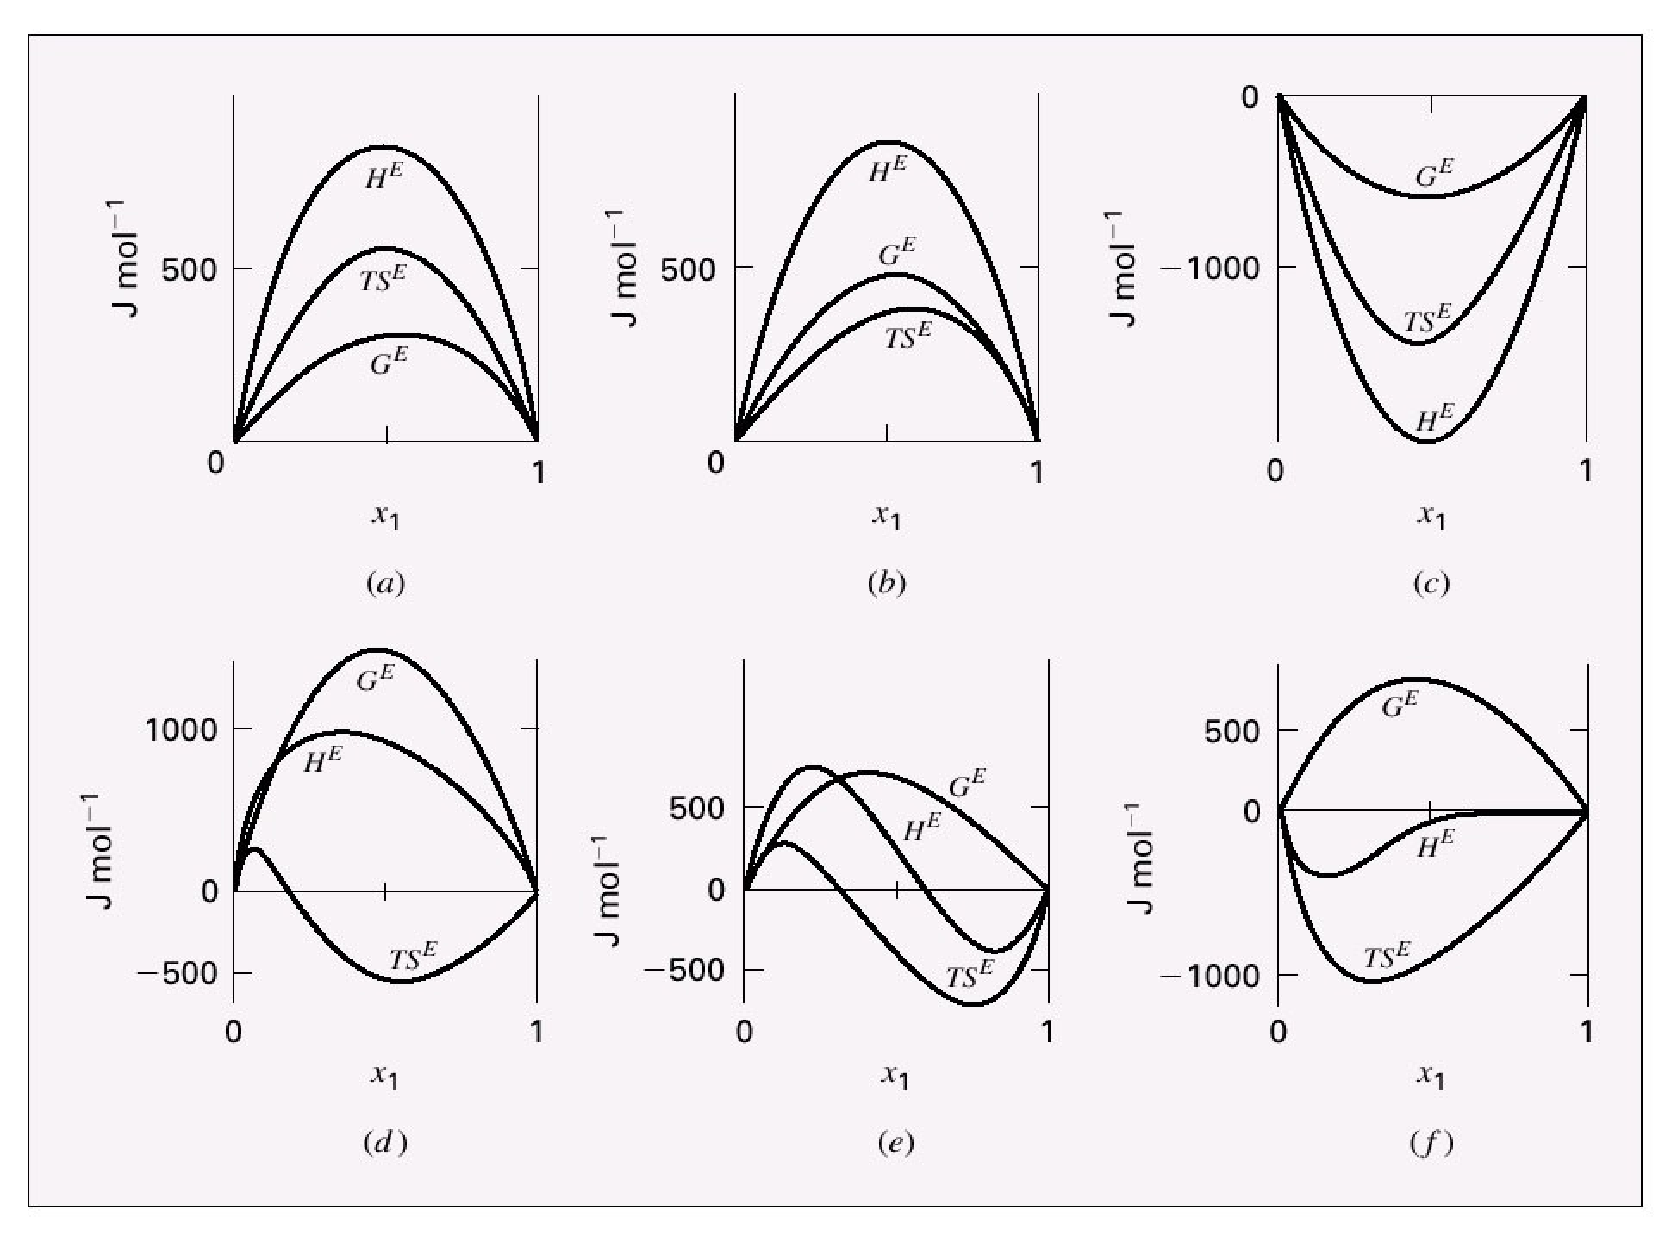
\includegraphics[width=9.cm, height=6.5cm,clip]{../Pics/ExcessProperties_Plot}
          \caption{\scriptsize Excess properties at 50$^{\circ}$C for the following binary liquid systems: (a) chloroform / n-heptane,(b) acetone / methanol, (c) acetone / chloroform, (d) ethanol / n-heptane, (e) ethanol / chloroform and (f) ethanol / water (Extracted from {\it Smith, Van Ness and Abott}). }
       \end{figure}
     \end{center}
\end{frame}
\normalsize


%%%
%%% SUBSECTION
%%%
\subsection{Activity Coefficient Models}

%%%
%%% Slide
%%%
%\scriptsize
\begin{frame}
  \frametitle{Activity Coefficient Models}
  \begin{enumerate}%\setcounter{enumi}{8}
      \item<1-> In several industrial and environmental applications EOS can not accurately predict the thermodynamic behaviour of solutions. In these cases, we can estimate the excess Gibbs energy \blue{$G^{\text{E}}$} (see Slide~\ref{ExcessProperty}, item~\ref{activitycoefficient}) by first calculating the activity coefficient, $\gamma_{i}$;
      \item<2-> Activity coefficient models are often more accurate (than traditional EOS) when strong intermolecular interactions are present;
      \item<3-> Models commonly used coefficient activity models in \blue{fluid simulators}:
          \begin{enumerate}
             \item<3-> Margules;
             \item<3-> Van Laar;
             \item<3-> Wilson;
             \item<3-> Non-Random-Two-Liquids (NRTL);
             \item<3-> UNIversal QUAsi Chemical (UNIQUAC).     
          \end{enumerate}
      \item<4-> Basic Equations:
          \visible<4->{\begin{displaymath}
            \gamma_{i} = \frc{\overline{f}_{i}}{x_{i}f_{i}}=\frc{\overline{f}_{i}}{\overline{f}_{i}^{\text{id}}},\hspace{1cm} \frc{G^{\text{E}}}{RT}=\xi\left(\gamma_{i}\right)
          \end{displaymath}
           where $\xi\left(\gamma_{i}\right)$ is a function of $\gamma_{i}$. Bear in mind that $\gamma_{i}$ is a function of composition, $x_{i}$. }
  \end{enumerate}
\end{frame}
\normalsize


%%%
%%% Slide
%%%
%\scriptsize
\begin{frame}
  \frametitle{Activity Coefficient Models}
  \begin{enumerate}\setcounter{enumi}{4}
      \item<1-> 2-parameter models for binary systems:
        \begin{enumerate}
          \item<1-> Mergules equations;
             \visible<1->{\begin{displaymath}
                \ln\gamma_{1}=x_{2}^{2}\left[A_{12}+2\left(A_{21}-A_{12}\right)x_{1}\right] \hspace{1cm} \ln\gamma_{2}=x_{1}^{2}\left[A_{21}+2\left(A_{12}-A_{21}\right)x_{2}\right]
             \end{displaymath}}
          \item<2-> Van Laar equations:
             \visible<2->{\begin{displaymath}
                \ln\gamma_{1}= B_{12}\left(1+\frc{B_{12}x_{1}}{A_{21}x_{2}}\right)^{-2}  \hspace{1cm} \ln\gamma_{2}= B_{21}\left(1+\frc{B_{21}x_{1}}{A_{12}x_{2}}\right)^{-2}
             \end{displaymath}}
          \item<3-> Wilson equations:
             \visible<3->{\begin{eqnarray}
                && \frc{G^{\text{E}}}{RT} = x_{1}\ln\left(x_{1}+x_{2}C_{12}\right) - x_{2}\ln\left(x_{2}+x_{1}C_{21}\right) \nonumber \\
                && \ln\gamma_{1}= -\ln\left(x_{1}+x_{2}C_{12}\right) + x_{2}\left(\frc{C_{12}}{x_{1}+x_{2}C_{12}}-\frc{C_{21}}{x_{2}+x_{1}C_{21}}\right)\nonumber \\
                && \ln\gamma_{2}= -\ln\left(x_{2}+x_{2}C_{21}\right) + x_{2}\left(\frc{C_{12}}{x_{1}+x_{2}C_{12}}-\frc{C_{21}}{x_{2}+x_{1}C_{21}}\right)\nonumber 
             \end{eqnarray}}
        \end{enumerate} 
  \end{enumerate}
\end{frame}
\normalsize


%%%
%%% Slide
%%%
%\scriptsize
\begin{frame}
  \frametitle{Activity Coefficient Models}
  \begin{enumerate}\setcounter{enumi}{5}
      \item<1-> NRTL and UNIQUAC are 3-parameter models that incorporate binary attraction/repulsion parameters of multiple chemical species;
       \item<2-> UNIFAC (UNIQUAC Functional-group Activity Coefficient) is a group contribution model that assign specific thermodynamic properties to functional group species, e.g., \red{$\cdot$CH$_{3}$}, \red{:CH$_{2}$}, \red{:COH}, \red{$\cdot$OH}, etc.
  \end{enumerate}
\end{frame}
\normalsize


%%%
%%% SECTION
%%%
\section{Summary}

%%%
%%% Slide
%%%
%\scriptsize
\begin{frame}
 \frametitle{Summary}
   \begin{enumerate}[(i)]
     \item Excess molar properties;
     \item Definition of activity,activity coefficient, fugacity, fugacity coefficient and chemical potential for pure species and mixtures;
     \item Brief description of activity coefficient models currently used in simulators.
   \end{enumerate}
\end{frame}

%%%
%%%  SECTION
%%%
\section{Examples}

%%%
%%% Slide
%%%
%\scriptsize 
\begin{frame}
 \frametitle{Example 1}\label{Ex1}
    \blue{At 25$^{\circ}$C and atmospheric pressure, the volume change of mixing of a binary liquid mixture of species 1 and 2 is given by,}
       \begin{displaymath}
          \blue{\Delta V = x_{1}x_{2}\left(45x_{1}+25x_{2}\right)\;\;\;\;\text{ with }\;\;\;\left[\Delta V\right] = \text{cm}^{3}.\text{mol}^{-1}}
       \end{displaymath}
       \blue{with molar volumes of $V_{1} = 110\;\text{cm}^{3}.\text{mol}^{-1}$ and $V_{2} = 90\;\text{cm}^{3}.\text{mol}^{-1}$. Determine the partial molar volumes, $\overline{V}_{1}$ and $\overline{V}_{2}$, in a mixture containing 40$\%$-mol of species 1.}

\end{frame}



\end{document}
 



\end{document}
